% main.tex – LaTeX-prosjekt for Digitale tvillinger i praksis for masterstudenter
\documentclass[12pt]{book}

% Pakker
\usepackage[utf8]{inputenc}
\usepackage[T1]{fontenc}
\usepackage{textcomp}
\usepackage{geometry}
\usepackage{graphicx}
\usepackage{hyperref}
\usepackage{array}
\usepackage{longtable}
\usepackage{booktabs}
\usepackage{enumitem}
\usepackage{verbatim}
\usepackage{xcolor}
\usepackage{tikz}
\usetikzlibrary{positioning,arrows.meta,fit}
\definecolor{dypblaa}{HTML}{1B4965}
\definecolor{petrol}{HTML}{2C7DA0}
\definecolor{havgronn}{HTML}{00A896}
\definecolor{solgul}{HTML}{F4D35E}
\definecolor{koral}{HTML}{EE6C4D}
\definecolor{grafitt}{HTML}{4F5D75}
\definecolor{skygraa}{HTML}{E5E9EC}
\usepackage[round,authoryear]{natbib}
\geometry{margin=1in}
\setlist{itemsep=0.5em}

% Metadata
\title{Digitale tvillinger i praksis for masterstudenter}
\author{Redaksjonen}
\date{\today}

\begin{document}

\frontmatter
\maketitle
\tableofcontents
\chapter*{Forord}
\addcontentsline{toc}{chapter}{Forord}

Digitale tvillinger har på kort tid etablert seg som en nøkkelkomponent i utviklingen av fremtidens produkter, tjenester og samfunnsinfrastruktur. Norske virksomheter står overfor et stort behov for kandidater som både forstår den teoretiske bakgrunnen og kan anvende teknologien i praksis. Denne boken er skrevet for masterstudenter som ønsker å bygge en solid kompetanseplattform som kombinerer modellering, dataanalyse, systemforståelse og organisatorisk innsikt.

Boken er strukturert i tre deler. Første del gir fundamentet gjennom begrepsforståelse, modellering og datahåndtering. Andre del fokuserer på metodikk, simulering og læring, mens tredje del knytter teorien til implementering, styring og norske case. Vi legger vekt på å presentere både teknisk dybde og refleksjon rundt etikk, bærekraft og endringsledelse.

Utviklingen av boken skjer iterativt. Vi inviterer lesere, studenter og fagmiljø til å bidra med erfaringer, eksempler og faglige innspill. Gjennom prosjektstrukturen som er beskrevet i \texttt{instruksjoner.md} og oppgaveoversikten i \texttt{\detokenize{task\_queue.md}}, kan vi sammen bygge en ressurs som støtter masterstudenter i å lykkes med digitale tvillinger i praksis.

\bigskip
\begin{flushright}
Redaksjonen
\end{flushright}


\mainmatter
\chapter{Introduksjon til digitale tvillinger}

\section{Læringsmål}
\begin{itemize}
    \item Forklare hva en digital tvilling er og hvordan begrepet har utviklet seg.
    \item Skille mellom digitale tvillinger, digitale skygger og klassiske simuleringsmodeller.
    \item Identifisere nøkkelkomponentene som trengs for å realisere en digital tvilling.
\end{itemize}

\section{Bakgrunn og definisjoner}
Begrepet «digital tvilling» dukket først opp i industrien rundt årtusenskiftet da Michael Grieves beskrev hvordan et fysisk produkt kunne speiles digitalt gjennom hele livssyklusen. NASA populariserte tankegangen tidlig på 2010-tallet som en videreføring av simulatorene de hadde brukt til Apollo-programmet og romfergen, der hver kritiske komponent hadde et matematisk «tvilling»-system som kunne testes i forkant av reelle operasjoner. Over tid har metoden blitt raffinert med økende datatilgang, IoT-infrastruktur og skytjenester som muliggjør kontinuerlig synkronisering mellom fysisk og digitalt system.

\subsection{Historiske milepæler}
Historien om digitale tvillinger springer ut av romfartens behov for å teste kritiske systemer på bakken før de ble sendt ut i verdensrommet. Simuleringsplattformene NASA utviklet for Apollo-programmet etablerte et tankesett der hver sentral komponent skulle ha et digitalt motstykke som muliggjorde analyse av feilscenarier og hurtige beslutninger underveis i oppdraget \citep{glaessgen2012digital}. I løpet av 2000-tallet ble ideen koblet til produktlivssyklusforvaltning (PLM), og begrepet «digital tvilling» ble popularisert i industrien.

\paragraph{Tidslinje i tekstform.} Siden tidligere TikZ-illustrasjon skapte kompilasjonsfeil, oppsummerer vi milepælene direkte i teksten nedenfor. Dette gir leseren samme informasjon uten behov for grafikk.

\begin{itemize}
    \item \textbf{1960--1970-tallet:} NASA utvikler speilende simuleringssystemer for Apollo og Skylab for å planlegge oppdrag og håndtere feilscenarier \citep{glaessgen2012digital}.
    \item \textbf{2002:} Michael Grieves lanserer digital tvilling-konseptet i PLM-litteraturen, og legger grunnlaget for dagens terminologi \citep{grieves2017digital}.
    \item \textbf{2010--2016:} NASA formaliserer Digital Twin-strategien, EU inkluderer konseptet i Horizon 2020-programmer, og ISO starter standardiseringsarbeid rundt industrielle datastrømmer.
    \item \textbf{2017:} Equinor introduserer digitale tvillinger for Johan Sverdrup-feltet for å kombinere sanntidsdata med historisk produksjonsinformasjon \citep{equinor2021johansverdrup}.
    \item \textbf{2018--2021:} Kongsberg Digital etablerer sin Kognitwin-plattform for prosessindustri, mens DNV og SINTEF samarbeider om normative rammeverk for digitale tvillinger i maritim sektor \citep{dnv2021rp,sintef2021digital}.
    \item \textbf{2024:} Norske kommuner tester bytvillinger for mobilitet, energi og klimatilpasning som del av omstillingsløp til grønnere byer \citep{trondheim2024bytvilling}.
\end{itemize}

Hvert trinn i tidslinjen over markerer både teknologiske og organisatoriske nyvinninger. Fra NASA sin vektlegging av redundant beslutningsstøtte til DNVs anbefalte praksis for industrielle tvillinger \citep{dnv2021rp} har begrepet gått fra å være et teknisk støtteverktøy til å bli en driver for helhetlig virksomhetsstyring. Norske pionerprosjekter, som Equinors Johan Sverdrup-tvillinger og Trondheim kommunes bytvilling for mobilitet, viser hvordan historiske erfaringer nå brukes til å balansere klimaambisjoner, sikkerhet og verdiskaping i offentlig sektor \citep{equinor2021johansverdrup,trondheim2024bytvilling}.

\subsection{Norske initiativer}
Norge har vært tidlig ute med å bruke digitale tvillinger i kritisk infrastruktur. Equinor, Aker BP og Gassco bruker teknologien for å optimalisere produksjon og vedlikehold på sokkelen, mens Statnett tester digitale kopier av kraftnettkomponenter for å simulere belastningstopper og planlegge nettiltak. I maritim sektor har Kongsberg Gruppen og DNV utviklet sertifiseringsløp og testfasiliteter, blant annet gjennom Ocean Space Centre i Trondheim. Kommunal sektor eksperimenterer med digitale tvillinger av bygg og byrom, slik som Statsbyggs modell for det nye regjeringskvartalet og Trondheim kommunes digitale tvilling av Sluppen-området for mobilitetsanalyse. Disse eksemplene viser hvordan historikken fra romfart og internasjonal industri har blitt tatt videre og tilpasset norske behov.

\subsection{Nøkkelbegreper}
En \emph{digital tvilling} omtales ofte som en digital representasjon av et fysisk system som er koblet til den virkelige enheten gjennom en kontinuerlig datautveksling. NASA vektlegger beslutningsstøtten som oppstår når modellen og den fysiske tvillingen lærer av hverandre, mens ISO 23247 og EU-kommisjonens veikart for industrielle tvillinger fremhever livssyklusperspektivet der utvikling, drift og avvikling henger sammen. I norsk kontekst brukes begrepet gjerne for å beskrive alt fra et detaljerte prosessanlegg til et helt byområde, men kjernen er alltid denne toveis forbindelsen mellom data, modell og fysisk verden.

Det er nyttig å skille mellom \emph{digital modell}, \emph{digital skygge} og \emph{digital tvilling}. En digital modell er en statisk representasjon --- for eksempel en BIM-modell --- som ikke nødvendigvis oppdateres når virkeligheten endrer seg. En digital skygge \textit{(digital shadow)} mottar sanntidsdata, men påvirker ikke det fysiske systemet tilbake. En digital tvilling går ett steg videre og muliggjør beslutninger som sendes tilbake i form av styringssignaler, vedlikeholdsoppdrag eller endrede operasjonsgrenser. Flere norske virksomheter, som Equinor og Statnett, har vært nøye med å bruke denne tredelingen for å tydeliggjøre modenhetsnivået i sine programmer.

I boken bruker vi konsekvent norske begreper der det finnes innarbeidede ord, men beholder engelske termer når de er bransjestandard. Dette betyr at leseren vil møte både «tilstandsestimering» og \emph{state estimation}, «tilbakeskriving» og \emph{backcasting}, samt «datainnsamlingsrør» og \emph{data pipelines}. Tabeller og figurer angir alltid begge språkvarianter første gang et begrep introduseres, slik at masterstudenter kan bevege seg sømløst mellom norske prosjekter og internasjonal litteratur.

\section{Økosystemet rundt digitale tvillinger}
En digital tvilling er mer enn modellen alene; den står på skuldrene til et helt økosystem av sensorer, kommunikasjon og dataplattformer. Sensorer og IoT-enheter etablerer det kontinuerlige sanntidsbildet som gjør at tvillingen kan oppdateres. På Johan Sverdrup-feltet kombineres vibrasjonsdata, trykkmålinger og produksjonsdata fra borebrønner i samme datastrøm før de kvalitetssikres og sendes til Equinors skyplattform. Tilsvarende har Bane NOR montert sensorer på kontaktledninger og sporfundament for å kunne simulere belastningsendringer i digitale tvillinger av jernbaneinfrastruktur.

Forbindelsen mellom det fysiske og det digitale håndteres ofte gjennom en såkalt \emph{digital thread}, et sett av datatjenester som binder sammen konstruksjonsdata, operative data og vedlikeholdslogger. Når Statnett utvikler tvillinger av transformatorstasjoner, hentes grunnlagsdata fra PLM-systemer, driftsdata fra SCADA, og risikomodeller fra analyseverktøy. Integrasjonen skjer via hendelsesdrevne API-er som sikrer at endringer i én del av økosystemet raskt reflekteres i tvillingen.

Teknologien alene er ikke nok. Domeneeksperter, dataingeniører og beslutningstakere må arbeide tverrfaglig for å etablere valide modeller og tolke resultatene. Trondheim kommunes mobilitetstvilling illustrerer dette: byplanleggere definerer hvilke scenarier som skal simuleres, dataforskere bygger trafikkmodellene, og tjenestedesignere vurderer hvordan innsikten skal brukes i medvirkningsprosesser med innbyggerne. Et velfungerende økosystem krever derfor tydelige roller, forvaltningsmodeller og kontinuerlig kompetansebygging.

\section{Verdiskaping og anvendelser}
Digitale tvillinger skaper verdi når de setter organisasjoner i stand til å handle raskere, tryggere og mer bærekraftig. I prosessindustrien brukes tvillinger til å optimalisere produksjonsparametere og redusere energiforbruk. Yara Porsgrunn rapporterer at de, gjennom en tvilling av ammoniakkfabrikken, kunne identifisere driftsvinduer som reduserte CO$_2$-utslipp med flere prosent uten å gå på akkord med sikkerheten. I maritim sektor benytter Kongsberg Digital sin \emph{Kognitwin}-plattform til å overvåke dynamisk posisjonering og drivstoffbruk på offshorefartøy, noe som gjør det mulig å planlegge vedlikehold før komponenter feiler.

Helsesektoren er i ferd med å ta i bruk digitale tvillinger av pasientforløp. Helseplattformen og NTNU har etablert pilotprosjekter der anonymiserte pasientdata brukes til å simulere behandlingsforløp for kronikere, slik at kliniske beslutninger kan støtte seg på sannsynlige utfall fremfor intuisjon alene. Slike løsninger gir ikke bare bedre ressursutnyttelse, men styrker også pasientsikkerheten ved å avdekke risikoer tidlig.

Verdiskapingen handler også om samfunnsmål. Digitale tvillinger av byrom, som Bodøs planlagte Smart Bodø-tvillingen, gir kommunene mulighet til å teste klimapolitikk og mobilitetsgrep før de implementeres. Når resultatene kobles med livssyklusanalyser og klima-rapportering, kan tvillingene dokumentere effekten av tiltak for utslippsreduksjoner og klimatilpasning. Dermed blir teknologien et verktøy for å levere på både økonomiske og bærekraftige mål, og masterstudenter får et tydelig bilde av hvordan teoretiske modeller oversettes til samfunnsnytte.

\subsection{Case: Johan Sverdrup som læringsplattform}
Equinor har brukt Johan Sverdrup-feltet som et testlaboratorium for integrerte arbeidsprosesser der digitale tvillinger kobles til vedlikeholdsplanlegging, produksjonsstyring og HMS-arbeid \citep{equinor2021johansverdrup}. Tvillingen kombinerer geologiske modeller, produksjonsdata og sensorer i brønnstrømmen slik at ingeniører kan simulere tiltak før de iverksettes offshore. Samtidig brukes modellen i dialog med leverandører for å evaluere nye komponenter etter DNVs anbefalte praksis \citep{dnv2021rp}. Tabell~\ref{tab:kap01-johan-sverdrup} oppsummerer hvordan dataflyt og organisering er bygget opp.

\begin{table}[ht]
    \centering
    \caption{Nøkkelkomponenter i Johan Sverdrup-tvillingen slik de brukes i Equinors læringsprogram.}
    \label{tab:kap01-johan-sverdrup}
    \begin{tabular}{p{0.32\textwidth}p{0.58\textwidth}}
        \toprule
        \textbf{Dimensjon} & \textbf{Beskrivelse} \\
        \midrule
        Datakilder & 1\,500 sanntidssensorer fra prosessanlegget, historiske produksjonskurver og integrasjon mot vedlikeholdssystem (SAP). \\
        Modellbibliotek & Fysikkbaserte reservoarmodeller, strømning i rør, maskinlæringsmodeller for pumpestatus og energioptimalisering. \\
        Arbeidsprosesser & Tverrfaglige «control rooms» med daglige simuleringsøkter og ukentlige forbedringsmøter med leverandører. \\
        Effekter & Redusert nedetid i kritiske kompressorer med 30\% og dokumentert utslippsreduksjon per fat produsert. \\
        Læringsarena & Brukes i masterkurs med deling av syntetiske datasett og scenarioer for risikotrening. \\
        \bottomrule
    \end{tabular}
\end{table}

\subsection{Case: Trondheim bylab for mobilitet}
Trondheim kommune kombinerer trafikkdata, klimascenarioer og innbyggerdialog i en bytvilling som brukes til å planlegge mobilitets- og energioppgradering i Sluppen-området \citep{trondheim2024bytvilling}. Tvillingen gjør det mulig å teste tiltak som ladeinfrastruktur, busslinjer og overvannshåndtering før investeringer besluttes. Innsikt fra modellen kobles til nasjonale klimamål og lokale budsjetter slik at politiske beslutninger kan dokumenteres.

\begin{table}[ht]
    \centering
    \caption{Faktorer Trondheim bylab vurderer ved bruk av digital tvilling for mobilitet.}
    \label{tab:kap01-trondheim}
    \begin{tabular}{p{0.35\textwidth}p{0.55\textwidth}}
        \toprule
        \textbf{Faktor} & \textbf{Utdyping} \\
        \midrule
        Datagrunnlag & Sanntid fra IoT-sensorer i vegbanen, kollektivdata fra AtB og klima-projeksjoner fra MET. \\
        Interessenter & Kommunal planavdeling, næringsliv, kollektivselskap og innbyggerpanel. \\
        Beslutningspunkter & Prioritering av sykkelveger, plassering av hurtigladere, rekkefølge på grønn infrastruktur. \\
        Visualisering & 3D-modell i kommunens dataplattform med scenario-dashboard og AR-visning i folkemøter. \\
        Resultater & Identifiserte 12\% potensial for energireduksjon i byggforvaltningen og redusert reisetid i rushtid med 8\%. \\
        \bottomrule
    \end{tabular}
\end{table}

Kombinasjonen av slike caser viser hvordan digitale tvillinger både støtter teknisk optimalisering og demokratiske prosesser når modellene brukes som en arena for samskaping.

\section{Refleksjonsspørsmål}
\begin{enumerate}
    \item Hvilke komponenter mener du er viktigst for å lykkes med en digital tvilling i ditt fagområde?
    \item Hvordan skiller en digital tvilling seg fra tradisjonelle simuleringsmodeller?
    \item Gi et eksempel på hvordan dataflyt påvirker verdien av en digital tvilling.
\end{enumerate}


\chapter{Systemtenkning og modellering}


\section{Læringsmål}
\begin{itemize}
    \item Analysere komplekse systemer ved hjelp av systemtenkning.
    \item Vurdere ulike modelleringsstrategier for digitale tvillinger.
    \item Beskrive hvordan modeller kobles til måledata og styringssystemer.
\end{itemize}

\section{Systemperspektiv}
Systemtenkning starter med å forstå hvilke deler av virkeligheten som påvirker hverandre og hvordan verdistrømmer beveger seg gjennom systemet. Første steg er å definere klare systemgrenser, identifisere interessenter og beskrive hva de forsøker å oppnå. Deretter kan vi visualisere samspillet mellom teknologi, prosesser og mennesker ved hjelp av systemkart, påvirkningsdiagrammer og kausale sløyfer. Figurene under gir to typiske fremstillinger for en digital tvilling i en norsk industribedrift.

\textbf{Nøkkelspørsmål når systemperspektivet etableres:}
\begin{itemize}
    \item Hvilke organisatoriske enheter og tekniske komponenter inngår i systemet?
    \item Hvilke datakilder, beslutninger og tilbakemeldingsløp knytter dem sammen?
    \item Hvilke målkonflikter kan oppstå mellom interessentene?
\end{itemize}

\subsection{Systemkart for produksjonslinje med digital tvilling}
% Alt-tekst: support/figurer/metadata/kap02-systemkart-v2.alt.md
\begin{figure}[ht]
    \centering
    \resizebox{\textwidth}{!}{% TikZ-figur: Systemkart for produksjonslinje med digital tvilling (versjon 2)
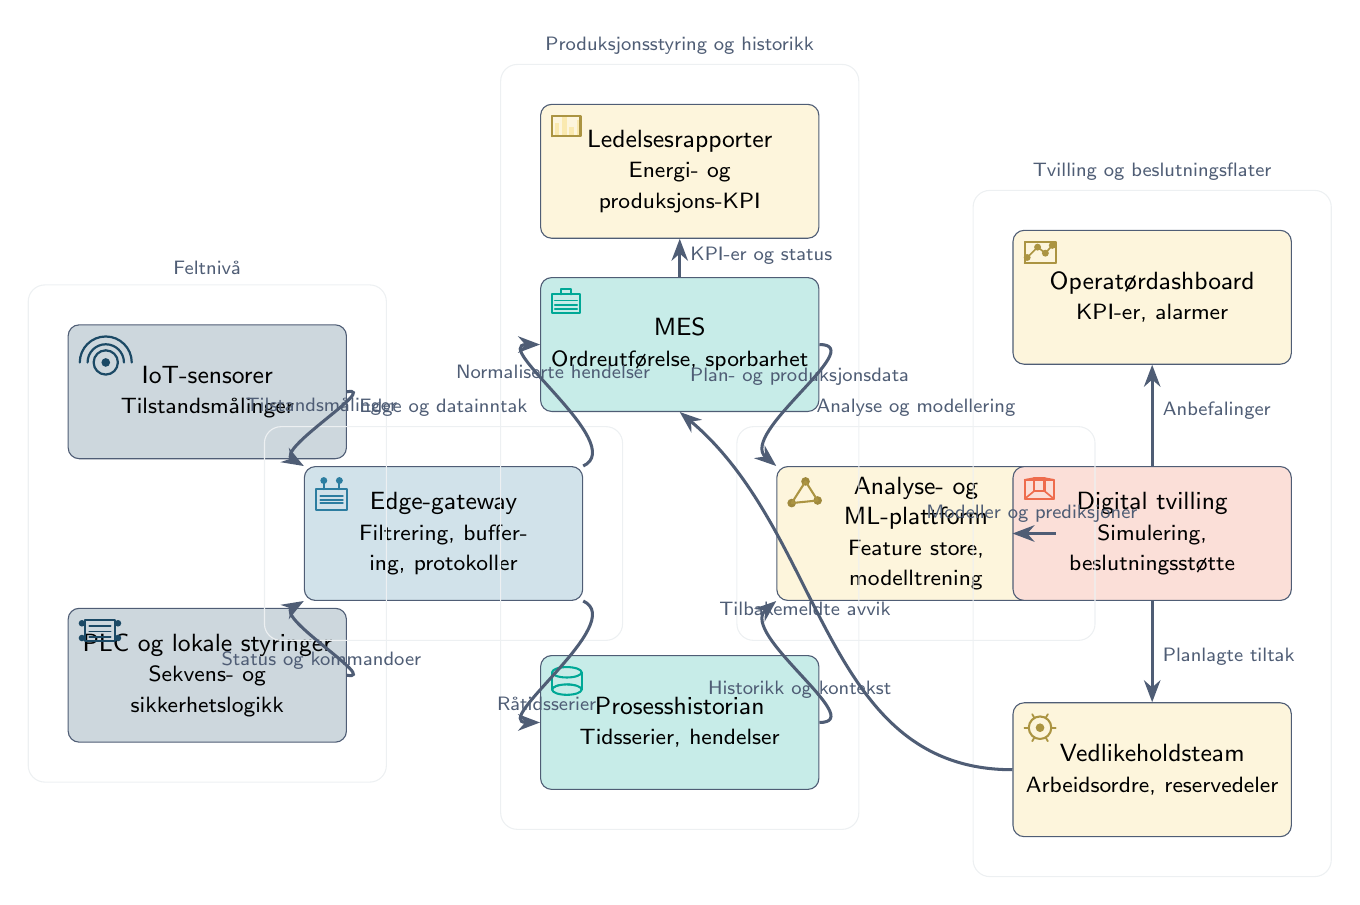
\begin{tikzpicture}[x=1cm, y=1cm, >=Stealth]
    \tikzset{
        module/.style={
            draw=grafitt,
            rounded corners=4pt,
            text width=3.3cm,
            minimum height=1.7cm,
            align=center,
            font=\small\sffamily,
            fill=#1!22
        },
        module/.default=skygraa,
        group/.style={
            draw=skygraa!70,
            rounded corners=6pt,
            inner sep=0.5cm
        },
        role/.style={
            font=\scriptsize\sffamily,
            text=grafitt
        },
        flow/.style={
            ->,
            line width=1.1pt,
            draw=grafitt
        }
    }

    \newcommand{\moduleicon}[3][0.55]{%%
        \node[anchor=north west, inner sep=1.8pt, xshift=2pt, yshift=-2pt] at (#2.north west) {%%
            \tikz[scale=#1, line cap=round, line join=round]{#3}
        };
    }

    % Noder
    \node[module=dypblaa]             (sensors)     at (0,  1.8) {IoT-sensorer\\\footnotesize Tilstandsm\aa linger};
    \node[module=dypblaa]             (plc)         at (0, -1.8) {PLC og lokale styringer\\\footnotesize Sekvens- og sikkerhetslogikk};
    \node[module=petrol]              (edge)        at (3,  0.0) {Edge-gateway\\\footnotesize Filtrering, buffering, protokoller};
    \node[module=havgronn]            (mes)         at (6,  2.4) {MES\\\footnotesize Ordreutf\o relse, sporbarhet};
    \node[module=havgronn]            (historian)   at (6, -2.4) {Prosesshistorian\\\footnotesize Tidsserier, hendelser};
    \node[module=solgul]              (analytics)   at (9,  0.0) {Analyse- og ML-plattform\\\footnotesize Feature store, modelltrening};
    \node[module=koral]               (dt)          at (12, 0.0) {Digital tvilling\\\footnotesize Simulering, beslutningsst\o tte};
    \node[module=solgul]              (dashboard)   at (12, 3.0) {Operat\o rdashboard\\\footnotesize KPI-er, alarmer};
    \node[module=solgul]              (maintenance) at (12,-3.0) {Vedlikeholdsteam\\\footnotesize Arbeidsordre, reservedeler};
    \node[module=solgul]              (management)  at (6,  4.6) {Ledelsesrapporter\\\footnotesize Energi- og produksjons-KPI};

    % Ikoner for modulene
    \moduleicon{sensors}{
        \draw[draw=dypblaa, line width=0.8pt] (0,0) circle (0.28);
        \draw[draw=dypblaa, line width=0.8pt] (0.42,0) arc (0:180:0.42);
        \draw[draw=dypblaa, line width=0.8pt] (0.6,0) arc (0:180:0.6);
        \fill[dypblaa] (0,0) circle (0.1);
    }
    \moduleicon[0.52]{plc}{
        \draw[draw=dypblaa, line width=0.85pt] (-0.36,-0.26) rectangle (0.36,0.26);
        \draw[draw=dypblaa, line width=0.65pt] (-0.26,0.12) -- (0.26,0.12);
        \draw[draw=dypblaa, line width=0.65pt] (-0.26,-0.02) -- (0.26,-0.02);
        \draw[draw=dypblaa, line width=0.65pt] (-0.26,-0.16) -- (0.26,-0.16);
        \fill[dypblaa] (-0.44,0.18) circle (0.08);
        \fill[dypblaa] (-0.44,-0.18) circle (0.08);
        \fill[dypblaa] (0.44,0.18) circle (0.08);
        \fill[dypblaa] (0.44,-0.18) circle (0.08);
    }
    \moduleicon{edge}{
        \draw[draw=petrol, line width=0.8pt] (-0.36,-0.24) rectangle (0.36,0.24);
        \draw[draw=petrol, line width=0.75pt] (-0.18,0.24) -- (-0.18,0.44);
        \draw[draw=petrol, line width=0.75pt] (0.18,0.24) -- (0.18,0.44);
        \fill[petrol] (-0.18,0.44) circle (0.08);
        \fill[petrol] (0.18,0.44) circle (0.08);
        \draw[draw=petrol, line width=0.65pt] (-0.26,-0.08) -- (0.26,-0.08);
        \draw[draw=petrol, line width=0.65pt] (-0.26,0.0) -- (0.26,0.0);
        \draw[draw=petrol, line width=0.65pt] (-0.26,0.08) -- (0.26,0.08);
    }
    \moduleicon{mes}{
        \draw[draw=havgronn, line width=0.75pt] (-0.32,-0.22) rectangle (0.32,0.22);
        \draw[draw=havgronn, line width=0.75pt] (-0.12,0.22) -- (-0.12,0.34) -- (0.12,0.34) -- (0.12,0.22);
        \draw[draw=havgronn, line width=0.6pt] (-0.26,0.08) -- (0.26,0.08);
        \draw[draw=havgronn, line width=0.6pt] (-0.26,-0.02) -- (0.26,-0.02);
        \draw[draw=havgronn, line width=0.6pt] (-0.26,-0.12) -- (0.26,-0.12);
    }
    \moduleicon{historian}{
        \draw[draw=havgronn, line width=0.75pt] (0,0.2) ellipse (0.34 and 0.12);
        \draw[draw=havgronn, line width=0.75pt] (0,-0.2) ellipse (0.34 and 0.12);
        \draw[draw=havgronn, line width=0.75pt] (-0.34,-0.2) -- (-0.34,0.2);
        \draw[draw=havgronn, line width=0.75pt] (0.34,-0.2) -- (0.34,0.2);
        \draw[dashed, draw=havgronn, line width=0.6pt] (-0.34,-0.2) arc[start angle=180, end angle=0, x radius=0.34, y radius=0.12];
    }
    \moduleicon{analytics}{
        \fill[solgul!65!black] (-0.3,-0.18) circle (0.1);
        \fill[solgul!65!black] (0.3,-0.12) circle (0.1);
        \fill[solgul!65!black] (0.02,0.32) circle (0.1);
        \draw[draw=solgul!70!black, line width=0.75pt] (-0.3,-0.18) -- (0.02,0.32) -- (0.3,-0.12) -- cycle;
    }
    \moduleicon{dt}{
        \draw[draw=koral, line width=0.75pt] (-0.34,-0.22) rectangle (0.34,0.22);
        \draw[draw=koral, line width=0.75pt] (-0.12,-0.04) rectangle (0.12,0.26);
        \draw[draw=koral, line width=0.6pt] (-0.34,-0.22) -- (-0.12,-0.04);
        \draw[draw=koral, line width=0.6pt] (0.34,-0.22) -- (0.12,-0.04);
        \draw[draw=koral, line width=0.6pt] (-0.34,0.22) -- (-0.12,0.26);
        \draw[draw=koral, line width=0.6pt] (0.34,0.22) -- (0.12,0.26);
        \draw[draw=koral, line width=0.6pt] (-0.12,-0.04) -- (0.12,-0.04);
    }
    \moduleicon{dashboard}{
        \draw[draw=solgul!70!black, line width=0.75pt] (-0.36,-0.24) rectangle (0.36,0.24);
        \draw[draw=solgul!70!black, line width=0.6pt] (-0.3,-0.12) -- (-0.06,0.12) -- (0.12,-0.02) -- (0.28,0.16);
        \fill[solgul!70!black] (-0.3,-0.12) circle (0.08);
        \fill[solgul!70!black] (-0.06,0.12) circle (0.08);
        \fill[solgul!70!black] (0.12,-0.02) circle (0.08);
        \fill[solgul!70!black] (0.28,0.16) circle (0.08);
        \draw[draw=solgul!70!black, line width=0.6pt] (-0.36,-0.24) -- (-0.36,0.24);
        \draw[draw=solgul!70!black, line width=0.6pt] (-0.36,-0.24) -- (0.36,-0.24);
    }
    \moduleicon{maintenance}{
        \foreach \angle in {0,60,...,300}{
            \draw[draw=solgul!70!black, line width=0.65pt] (\angle:0.26) -- (\angle:0.36);
        }
        \draw[draw=solgul!70!black, line width=0.75pt] (0,0) circle (0.26);
        \fill[solgul!70!black] (0,0) circle (0.1);
    }
    \moduleicon[0.5]{management}{
        \fill[solgul!50!white] (-0.3,-0.24) rectangle (-0.18,0.08);
        \fill[solgul!50!white] (-0.1,-0.24) rectangle (0.02,0.24);
        \fill[solgul!50!white] (0.08,-0.24) rectangle (0.2,-0.02);
        \fill[solgul!50!white] (0.26,-0.24) rectangle (0.38,0.16);
        \draw[draw=solgul!70!black, line width=0.75pt] (-0.36,-0.26) rectangle (0.36,0.26);
        \draw[draw=solgul!70!black, line width=0.6pt] (-0.36,-0.26) -- (-0.36,0.26);
        \draw[draw=solgul!70!black, line width=0.6pt] (-0.36,-0.26) -- (0.36,-0.26);
    }

    % Grupper
    \node[group, label={[role]north:Feltniv\aa}]                      at (0, 0)     (fieldbox)     [fit=(sensors)(plc)] {};
    \node[group, label={[role]north:Edge og datainntak}]              at (3, 0)     (edgebox)      [fit=(edge)] {};
    \node[group, label={[role]north:Produksjonsstyring og historikk}] at (6, 0.8)   (mesbox)       [fit=(mes)(historian)(management)] {};
    \node[group, label={[role]north:Analyse og modellering}]          at (9, 0)     (analyticsbox) [fit=(analytics)] {};
    \node[group, label={[role]north:Tvilling og beslutningsflater}]   at (12, 0)    (dtbox)        [fit=(dt)(dashboard)(maintenance)] {};

    % Piler
    \draw[flow] (sensors.east)     to[out=10,  in=150] node[role, pos=0.55, above] {Tilstandsm\aa linger} (edge.north west);
    \draw[flow] (plc.east)         to[out=-10, in=210] node[role, pos=0.55, below] {Status og kommandoer} (edge.south west);
    \draw[flow] (edge.north east)  to[out=25, in=180]  node[role, pos=0.55, above] {Normaliserte hendelser} (mes.west);
    \draw[flow] (edge.south east)  to[out=-25,in=180]  node[role, pos=0.6, below] {R\aa tidsserier} (historian.west);
    \draw[flow] (mes.east)         to[out=0,   in=140] node[role, pos=0.52, above] {Plan- og produksjonsdata} (analytics.north west);
    \draw[flow] (historian.east)   to[out=0,   in=-140] node[role, pos=0.52, below] {Historikk og kontekst} (analytics.south west);
    \draw[flow] (analytics.east)   --                         node[role, pos=0.55, above] {Modeller og prediksjoner} (dt.west);
    \draw[flow] (dt.north)         --                         node[role, pos=0.55, right] {Anbefalinger} (dashboard.south);
    \draw[flow] (dt.south)         --                         node[role, pos=0.55, right] {Planlagte tiltak} (maintenance.north);
    \draw[flow] (maintenance.west) to[out=180, in=-40] node[role, pos=0.6, below] {Tilbakemeldte avvik} (mes.south);
    \draw[flow] (mes.north)        --                         node[role, pos=0.55, right] {KPI-er og status} (management.south);
\end{tikzpicture}
}
    \caption{Systemkart som viser hvordan data flyter fra felt via edge- og produksjonsstyringslag til analyseplattformer og digitale tvillingtjenester. Ikonene markerer hovedtypen av komponent i hvert lag.}
    \label{fig:kap02-systemkart}
\end{figure}

Figur~\ref{fig:kap02-systemkart} illustrerer et typisk informasjonsløp der feltnivå, edge-infrastruktur og produksjonsstyringssystemer er tydelig gruppert. Ikonene i boksen peker på om elementet er en fysisk enhet, en styringsapplikasjon eller et analyse-/beslutningsgrensesnitt, slik at ansvarsdelingen blir enklere å lese. Historiske data kombineres med analyseplattformen for å oppdatere den digitale tvillingen, som igjen leverer beslutningsstøtte til operatører, vedlikeholdsteam og ledelse. Når du lager et eget systemkart, noter eksplisitt hvilke datatyper som flyter mellom nodene, og marker hvor ansvar og eierskap ligger i hvert lag.

\subsection{Kausalsløyfe mellom vedlikehold og energibruk}
% Alt-tekst: support/figurer/metadata/kap02-kausal-v1.alt.md
\begin{figure}[ht]
    \centering
    \resizebox{0.92\textwidth}{!}{% TikZ-figur: Kausalsl\o yfe mellom vedlikehold og energibruk (versjon 1)
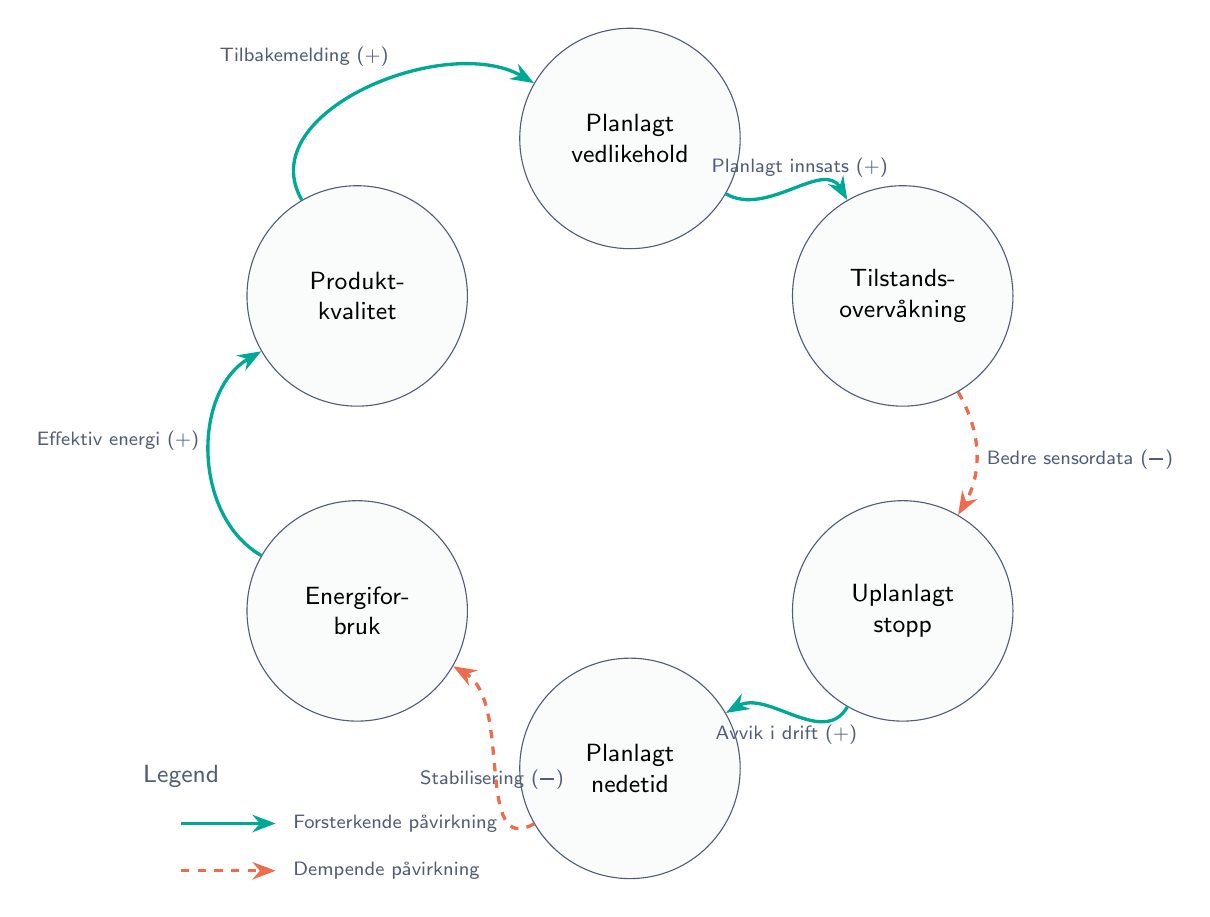
\begin{tikzpicture}[>=Stealth]
    \tikzset{
        loopnode/.style={
            draw=grafitt,
            circle,
            minimum size=2.8cm,
            align=center,
            font=\small\sffamily,
            fill=skygraa!20
        },
        posarrow/.style={
            ->,
            draw=havgronn,
            line width=1.2pt
        },
        negarow/.style={
            ->,
            draw=koral,
            dashed,
            line width=1.2pt
        },
        lab/.style={
            font=\scriptsize\sffamily,
            text=grafitt
        }
    }

    % Noder plassert p\aa sirkel
    \def\radius{4.0}
    \node[loopnode] (maint)      at (90:\radius)  {Planlagt\\vedlikehold};
    \node[loopnode] (monitor)    at (30:\radius)  {Tilstands-\\overv\aa kning};
    \node[loopnode] (stopp)      at (-30:\radius) {Uplanlagt\\stopp};
    \node[loopnode] (downtime)   at (-90:\radius) {Planlagt\\nedetid};
    \node[loopnode] (energy)     at (-150:\radius){Energifor-\\bruk};
    \node[loopnode] (quality)    at (150:\radius) {Produkt-\\kvalitet};

    % Piler med påvirkning
    \draw[posarrow] (maint)      to[out=-30, in=120] node[lab, pos=0.55, above] {Planlagt innsats (+)} (monitor);
    \draw[negarow] (monitor)     to[out=-60, in=60]  node[lab, pos=0.55, right] {Bedre sensordata (\textminus)} (stopp);
    \draw[posarrow] (stopp)      to[out=-120,in=30]  node[lab, pos=0.55, below] {Avvik i drift (+)} (downtime);
    \draw[negarow] (downtime)    to[out=-150,in=-30] node[lab, pos=0.55, below] {Stabilisering (\textminus)} (energy);
    \draw[posarrow] (energy)     to[out=150, in=-150] node[lab, pos=0.55, left] {Effektiv energi (+)} (quality);
    \draw[posarrow] (quality)    to[out=120, in=150] node[lab, pos=0.6, above left] {Tilbakemelding (+)} (maint);

    % Legend
    \begin{scope}[shift={(-5.7,-4.7)}]
        \node[lab, font=\small\sffamily] at (0,0.6) {Legend};
        \draw[posarrow] (0,0) -- (1.2,0);
        \node[lab, anchor=west] at (1.3,0) {Forsterkende p\aa virkning};
        \draw[negarow] (0,-0.6) -- (1.2,-0.6);
        \node[lab, anchor=west] at (1.3,-0.6) {Dempende p\aa virkning};
    \end{scope}
\end{tikzpicture}
}
    \caption{Forsterkende (grønn) og dempende (oransje) sammenhenger mellom planlagt vedlikehold, tilstandsovervåkning, nedetid, energiforbruk og produktkvalitet.}
    \label{fig:kap02-kausal}
\end{figure}

Kausalsløyfen i figur~\ref{fig:kap02-kausal} viser hvordan systemkart kan brukes til å fange både ønskede og uønskede tilbakemeldinger. Økt planlagt vedlikehold forbedrer sensorenes status, som reduserer risiko for uplanlagte stopp og stabiliserer energibruken. Et stabilt energinivå gir høyere produktkvalitet, noe som igjen påvirker vedlikeholdsstrategien gjennom læring og prioritering av tiltak. Når slike forhold beskrives eksplisitt, blir det enklere å diskutere scenarier med interessenter og identifisere hvor den digitale tvillingen bør levere mest verdi.

\textbf{Arbeidsmåte for å utvikle systemkart:}
\begin{enumerate}
    \item Start med en workshop hvor interessenter beskriver mål og smertepunkter.
    \item Tegn det overordnede systemkartet (som i Figur 2.1) med fokus på dataflyt og ansvar.
    \item Utvid kartet med kausale sløyfer (som i Figur 2.2) for å avdekke dynamikk og mulige ubalanser.
    \item Forankre kartene i virksomhetens enterprise-arkitektur og eksisterende prosesskart slik at språk og symboler er gjenkjennelige for organisasjonen.
\end{enumerate}

Den konseptuelle modellen fra systemkartet danner grunnlaget for videre modellering, enten du velger fysikkbaserte, datadrevne eller hybride tilnærminger i de følgende seksjonene.

\section{Modelleringsparadigmer}
Systemkartet gir en felles forståelse av hvilke fenomener som må representeres i en digital tvilling. Neste steg er å velge et
modelleringsparadigme som balanserer nøyaktighet, forklarbarhet og implementasjonskostnad. Masterstudenter må kunne vurdere
hvordan ulike typer modeller beskriver sammenhengene i systemet og hvilke beslutninger de støtter. I praksis innebærer dette å
kombinere domenekunnskap fra feltet med metoder fra matematikk, statistikk og informatikk.

\subsection{Fysikkbaserte modeller}
Fysikkbaserte modeller er bygd på eksplisitte ligninger som beskriver energi-, masse- eller informasjonsstrømmer. Typiske
teknikker er differensialligninger, finite element-metoder (FEM) og computational fluid dynamics (CFD). Fordelen er at
modellene er transparente og muliggjør følsomhetsanalyser, men de krever inngående forståelse av prosessen og god kvalitet på
parametere. I norske prosessindustrier brukes slike modeller blant annet til å simulere varmebalanser i ovner, fukttransport i
trebaserte materialer og hydrodynamikk i fiskemerder.

\subsection{Datadrevne modeller}
Datadrevne modeller lærer systemets oppførsel direkte fra historiske eller sanntidsdata. Maskinlæring og statistiske metoder
kan identifisere mønstre uten å kjenne den underliggende fysikken. En digital skygge kan trenes på tidsserier fra sensorer for
å predikere avvik i produksjonen. Fordelen er rask implementering når rike datasett finnes, men modellene kan bli sårbare for
driftsendringer og må overvåkes for skjevheter.

\subsection{Hybride modeller og ko-simulering}
I mange digitale tvillinger kombineres fysikkbaserte og datadrevne komponenter. En hybrid modell kan bruke førsteprinsipper for
energi- og materialbalanser, mens maskinlæring estimerer friksjonstap eller operatørpåvirkning som er vanskelig å beskrive
analytisk. Ko-simulering gjør det mulig å koble sammen flere spesialiserte modeller i en helhetlig tidslinje, for eksempel når
mekanikk, termodynamikk og styringslogikk må løses samtidig \citep{boschert2018digital}. Denne kombinasjonen gir robusthet og
fleksibilitet, men krever tydelige API-kontrakter, delte dataskjema og versjonskontroll av hvert delsystem.

\subsection{Flerfidelitetsstrategier}
Flerfidelitetsmodellering kombinerer raske, grovkornede modeller med detaljerte høyfidelitetsmodeller for kritiske delsystemer.
Lavfidelitetsmodellen gir raske scenarioberegninger og støtte til beslutninger med stramme tidsfrister, mens høyfidelitetsmodellen
brukes til kalibrering og validering av sentrale parametere \citep{kennedy2000predicting}. Strategien er særlig nyttig i norsk
prosess- og energisektor der tilgangen til sensordata varierer mellom installasjoner \citep{sintef2021digital}. Et vellykket
flerfidelitetsoppsett krever at teamet:
\begin{itemize}
    \item definerer hvilke variabler som skal utveksles mellom modellene og hvordan usikkerhet skal rapporteres,
    \item etablerer en synkroniseringsplan for når høyfidelitetsmodellen skal oppdateres og hvordan endringene mates inn i
    lavfidelitetsmodellen,
    \item dokumenterer toleranser for avvik slik at driftsorganisasjonen vet når det er nødvendig med ny kalibrering eller
    eksperimentelle målinger.
\end{itemize}

\subsection{Case: Flerfidel modell for subsea-kompressorer}
Et norsk leverandørkonsortium har utviklet en digital tvilling for subsea-kompressorer på sokkelen. Plattformen kombinerer en
hurtig maskinlæringsmodell som estimerer produksjon og energiforbruk fra tilgjengelige trykk- og temperaturmålinger, med en
høyfidel CFD-modell som simulerer detaljerte turbulenseffekter i kompressoren. Hver natt kjøres CFD-modellen mot oppdaterte
operasjonsdata for å korrigere parametere i hurtigmodellen. Resultatene deles med driftsteamet gjennom et dashboard der
avvik merkes når usikkerheten overstiger definerte grenser. Prosjektet viser hvordan flerfidelitetsstrategier gir bedre
tilgjengelighet og vedlikeholdsplanlegging samtidig som modellene er dokumentert og revideres i samarbeid mellom operatør og
teknologipartnere \citep{sintef2021digital}.

\subsection{Vurdering av modellvalg}
Når et paradigme skal velges, bør teamet diskutere hvor kritisk forklarbarhet er, hvilke datakilder som er tilgjengelige og hvor
raskt modellen må oppdateres. Tabell~\ref{tab:kap02-modellvalg} gir et utgangspunkt for å sammenligne alternativer og velge en
portefølje av modeller som utfyller hverandre.

\begin{table}[ht]
    \centering
    \caption{Sammenligning av modelleringsparadigmer for digitale tvillinger.}
    \label{tab:kap02-modellvalg}
    \begin{tabular}{p{0.2\textwidth}p{0.27\textwidth}p{0.24\textwidth}p{0.23\textwidth}}
        \toprule
        \textbf{Paradigme} & \textbf{Styrker} & \textbf{Utfordringer} & \textbf{Typisk norsk case} \\
        \midrule
        Fysikkbasert & Forklarbare sammenhenger og mulighet for sensitivitetstester. & Krever detaljerte parametere og høy beregningskostnad. & Energiproduksjon med krav til termisk balanse. \\
        Datadrevet & Rask modellering når historiske data er rike. & Sårbar for konseptdrift og bias i data. & Produksjonslinjer med omfattende sensordekning. \\
        Hybrid & Kombinerer robusthet og fleksibilitet gjennom ko-simulering. & Krever koordinering av grensesnitt og felles semantikk. & Integrerte olje- og gassanlegg med flere disipliner. \\
        Agent-/hendelsesbasert & Fanger interaksjon mellom aktører og logistikkflyt. & Vanskelig å kalibrere uten detaljerte prosesslogger. & Transport- og beredskapsøvelser på lufthavner. \\
    \end{tabular}
\end{table}

I praksis bør valget dokumenteres i en modelljournal som beskriver antagelser, datakrav og ansvarlige personer for videre vedlikehold
\citep{iso23247-2021}. Dokumentér alltid hvilke måledata som trengs for å holde modellen presis over tid og hvordan modellene skal
gjennomgås i fagfelleprosesser.

\section{Modellintegrasjon og kalibrering}
Valgt modell må kobles til dataflyten som ble kartlagt tidligere. Integrasjon handler både om teknisk infrastruktur og
organisatorisk forankring. Kalibrering sikrer at modellen forblir relevant når systemet endrer seg.

\subsection{Integrasjonsmønstre mot datakilder}
Modellen kan oppdateres batchvis fra historiske datalagre eller kontinuerlig via hendelsesstrømmer. Et vanlig mønster er å bruke
en meldingskø eller et datamesh som mellomlag, slik at flere modeller kan abonnere på samme datasett uten å skape tette koblinger
til kildesystemene. Edge-komponenter håndterer ofte aggregering og filtrering før data sendes til skybaserte analyseplattformer.

\subsection{Sanntidsoppdatering og orkestrering}
For digitale tvillinger som støtter operativ beslutningstaking må modellene ha mekanismer for å oppdatere tilstandsvariabler i
sanntid. Dette kan løses med orkestreringsverktøy som støtter versjonering av modeller, utrulling i containere og overvåkning av
beregningstider. Viktige indikatorer er latens fra sensor til modell, datakvalitet og hvilken grad modellen brukes i kontrollsløyfer.

\subsection{Kalibreringsstrategier}
Parameteridentifikasjon kan gjøres manuelt ved å justere parameterne basert på eksperterfaring, eller automatisk ved hjelp av
optimaliseringsalgoritmer som minimerer forskjellen mellom modell og målinger. Vanlige metoder er minste kvadrater,
Bayesiansk oppdatering eller Kalman-filtre. For systemer som endrer seg gradvis kan modellreduksjon og adaptive filtre holde
beregningstidene nede uten å tape presisjon. Tabell~\ref{tab:kap02-kalibrering} viser hvordan ulike kalibreringsteknikker kan
kombineres for å støtte flerfidelitetsmodeller og operativ drift \citep{kennedy2000predicting}.

\begin{table}[ht]
    \centering
    \caption{Oversikt over kalibreringsmetoder for digitale tvillinger.}
    \label{tab:kap02-kalibrering}
    \begin{tabular}{p{0.2\textwidth}p{0.32\textwidth}p{0.2\textwidth}p{0.22\textwidth}}
        \toprule
        \textbf{Metode} & \textbf{Formål} & \textbf{Når brukes den?} & \textbf{Typisk dokumentasjon} \\
        \midrule
        Minste kvadrater & Justere parametere basert på referansemålinger. & Ved innkjøring av nye sensorer eller komponenter. & Måleserier, residuallogg og parameteroversikt. \\
        Bayesiansk oppdatering & Kombinere historisk kunnskap med nye observasjoner. & Når usikkerhet skal uttrykkes eksplisitt og modeller skal sammenliknes. & Prior- og posteriorfordelinger samt versjonslogg. \\
        Kalman-filtre & Sanntidsestimater av tilstand og støy. & I operativ drift med streamingdata og krav til rask respons. & Konfigurasjon av filter, kovariansmatriser og alarmintervaller. \\
        Eksperimentell design & Planlegge testkampanjer for flerfidelitetsmodeller. & Før modelloppdateringer i laboratorier eller testfelt. & Testplan, datakvalitetsprotokoll og risikovurdering. \\
    \end{tabular}
\end{table}

Dokumentasjonen må vise hvilke datasett som ligger til grunn, hvordan datakvalitet er vurdert og hvilke roller som godkjenner nye
parameterverdier før de tas i bruk i produksjon.

\subsection{Case: Digital tvilling for fjernvarme i Oslo}
Fortum Oslo Varme har utviklet en digital tvilling for å optimalisere energiproduksjon og distribusjon i fjernvarmenettet.
Modellen kombinerer hydrauliske ligninger for rørnettet med maskinlæringsmodeller som predikerer varmebehov basert på vær,
bygningstyper og historisk forbruk. Integrasjonen skjer via en datastrøm fra sensorer i kundesentraler og produksjonsanlegg til
et skybasert kontrollrom. Kalibreringen utføres daglig ved å sammenlikne modellprediksjoner med faktiske returtemperaturer, og
parametere justeres automatisk når avvik overstiger definerte terskler. Caset viser hvordan samarbeid mellom energiselskap,
teknologipartnere og kommune gir en robust modell som støtter både operativ drift og langsiktige investeringsbeslutninger.

\subsection{Anbefalt arbeidsflyt for team}
\begin{enumerate}
    \item Kartlegg hvilke datakilder som skal kobles til og etabler nødvendige API-er eller databrokere.
    \item Implementer monitorering som fanger avvik mellom modell og observasjoner i sanntid.
    \item Planlegg regelmessige kalibreringssykluser og dokumentér endringer i parametere og antagelser.
\end{enumerate}

\section{Modelldokumentasjon og styring}
God dokumentasjon sikrer at digitale tvillinger kan forvaltes over tid og at beslutninger er etterprøvbare. ISO~23247 beskriver hvordan modellbeskrivelser, datakataloger og styringsrutiner bør struktureres for produksjonsnære tvillinger \citep{iso23247-2021}. Ved å etablere en felles dokumentasjonsprosess blir det enklere å dele modeller på tvers av fagmiljø og følge opp krav fra myndigheter og industripartnere.

\subsection{Kjerneartefakter}
Hvert modelloppsett bør følges av en artefaktsamling som minimum inneholder:
\begin{itemize}
    \item \textbf{Modelljournal} med formål, antagelser, matematiske representasjoner og referanse til opplæringsdata.
    \item \textbf{Datakatalog} som beskriver kilder, oppdateringsfrekvens, kvalitetsindikatorer og tilgangsnivå.
    \item \textbf{Beslutningslogg} som kobler modellresultater til tiltak, ansvarlige personer og godkjenningstidspunkt.
    \item \textbf{Risikovurdering} som fanger opp driftsavvik, cybersikkerhetskrav og konsekvenser av modellfeil.
\end{itemize}

\subsection{Versjonskontroll og sporbarhet}
Alle modeller bør ligge i et versjonsstyrt repositorium der kode, parametere og dokumentasjon utvikles samlet. Metadata for hver versjon må beskrive hvilke datasett og kalibreringsmetoder som er brukt, samt referanser til godkjenning og testresultater. For hybride og flerfidelitetsmodeller innebærer dette at også grensesnittfiler og transformasjoner sjekkes inn, slik at ko-simulering kan reproduseres ved behov \citep{boschert2018digital}. Kombiner gjerne Git-baserte prosesser med automatisert rapportering fra modellovervåkingen for å vise status i sanntid.

\subsection{Sjekkliste før fagfellegjennomgang}
Før en modell distribueres til undervisning eller pilotering, bør teamet kontrollere følgende punkter:
\begin{enumerate}
    \item Alle kilder og referanser er oppdatert i modelljournalen, og versjonsnummer samsvarer med distribuerte pakker.
    \item Kalibreringsresultater og usikkerhetsanalyser er lagret sammen med underliggende datasett og beskrivelser av kvalitetssikring.
    \item Tiltak for sikker tilgang, personvern og beredskap er dokumentert, inkludert roller og kontaktpunkter for hendelseshåndtering.
    \item Plan for kontinuerlig forbedring er definert med milepæler, måleparametere og ansvarlig fagressurs.
\end{enumerate}

\section{Norske politiske rammer}
Digitale tvillinger i Norge utvikles innenfor et politisk landskap som legger tydelige føringer for hvordan data skal forvaltes, deles og brukes. Regjeringens datastrategi for offentlig sektor legger vekt på åpne, tilgjengelige og gjenbrukbare data som skal styrke innovasjon og effektivisering \citep{regjeringen2022datastrategi}. I tillegg beskriver stortingsmeldingen \emph{Data som ressurs} hvordan sektorer må samhandle gjennom felles prinsipper for datadeling, sikkerhet og personvern \citep{meldst22datasomressurs}. Figuren under viser hvordan europeiske, nasjonale og sektorspesifikke initiativ henger sammen når virksomheter planlegger digitale tvillinger.

\begin{figure}[ht]
    \centering
    \resizebox{0.9\textwidth}{!}{\begin{tikzpicture}[box/.style={rectangle, rounded corners, draw=grafitt, thick, fill=skygraa!40, minimum width=4cm, minimum height=1.6cm, align=center}, connector/.style={-Latex, thick, petrol}]
    \node[box, fill=petrol!20] (eu) {EU-initiativ\nGaia-X, dataspace-rammer\citep{eu2020circulareconomy}};
    \node[box, below=1.2cm of eu, fill=solgul!40] (national) {Nasjonale strategier\nMeld. St. 22 (2020--2021) og digitaliseringsstrategi\citep{meldst22datasomressurs,regjeringen2022datastrategi}};
    \node[box, below left=1.4cm and 1.2cm of national, fill=havgronn!35] (energy) {Energisektor\nNVE retningslinjer for nettplanlegging\citep{nve2023nettplan}};
    \node[box, below=1.4cm of national, fill=havgronn!35] (transport) {Transport\nNTP-oppfølging og Avinor digitaliseringsplan\citep{avinor2022digital}};
    \node[box, below right=1.4cm and 1.2cm of national, fill=havgronn!35] (built) {Bygg og by\nPlan- og bygningslov, klimabudsjett\citep{trondheim2024bytvilling}};
    \node[box, below=1.2cm of energy, fill=white] (organisation) {Virksomhetsnivå\nProsesskrav, datakvalitet og fagfelleløp};

    \draw[connector] (eu) -- (national);
    \draw[connector] (national.south west) to[out=-110, in=90] (energy.north);
    \draw[connector] (national.south) -- (transport.north);
    \draw[connector] (national.south east) to[out=-70, in=90] (built.north);
    \draw[connector] (energy) -- (organisation);
    \draw[connector] (transport) -- (organisation);
    \draw[connector] (built) -- (organisation);
\end{tikzpicture}
}
    \caption{Sammenhengen mellom europeiske initiativ, nasjonale strategier og sektorspesifikke reguleringer som påvirker digitale tvillingprosjekter.}
    \label{fig:kap02-politikk}
\end{figure}

\subsection{Statlige føringer og standardisering}
EU sitt arbeid med datarom og Gaia-X gir retningslinjer for interoperabilitet, sikker tilgang og styring av dataøkosystem \citep{eu2020circulareconomy}. Disse prinsippene videreføres i nasjonale strategier og i oppfølgingen av personvern-, sikkerhets- og energilovgivning. For digitaliseringsprosjekter i offentlig sektor betyr det at arkitekturen må støtte datadeling på tvers av etater, samtidig som den ivaretar krav til informasjonssikkerhet gjennom standarder som ISO~27001 og NIS2. NVE og Samferdselsdepartementet stiller tilsvarende krav i sektorveiledninger for energi og transport \citep{nve2023nettplan,avinor2022digital}.

\subsection{Case: Statnett sitt nettplanleggingsprogram}
Statnett bruker digitale tvillinger til å planlegge nettutbygging og driftsoptimalisering i takt med økende elektrifisering. Plattformen integrerer kraftsystemmodeller, sanntidsmålinger og scenarioer for energioverganger og må følge både energiloven og nye EØS-krav til datasamarbeid \citep{statnett2023digital}. Caset illustrerer hvordan politiske føringer styrer både modellstrukturen og arbeidsprosessene.

\begin{table}[ht]
    \centering
    \caption{Regulatoriske og tekniske komponenter i Statnett sitt nettplanleggingsprogram.}
    \label{tab:kap02-statnett}
    \begin{tabular}{p{0.33\textwidth}p{0.57\textwidth}}
        \toprule
        \textbf{Komponent} & \textbf{Beskrivelse} \\
        \midrule
        Regulatorisk ramme & Energimyndighetenes konsesjonskrav, NVE sin veileder for nettplanlegging og krav til samfunnsøkonomiske analyser. \\
        Dataintegrasjon & PMU-målinger og SCADA-data kobles med langsiktige forbruksprognoser og markedsdata. \\
        Beslutningsfora & Tverretatlige møter med NVE og OED hver kvartal for å evaluere scenarioer og prioriteringer. \\
        Effektmåling & Reduserte flaskehalser, bedre koordinering med regionale nettselskap og dokumentert klimanytte i investeringsbeslutninger. \\
        Kompetansebygging & Kurs i regulatoriske krav og modellbruk for Statnett-ansatte og samarbeidspartnere. \\
        \bottomrule
    \end{tabular}
\end{table}

Caset viser hvordan systemkart og modellvalg må reflektere både tekniske og regulatoriske perspektiver. Ved å knytte datastrømmer til konkrete konsesjonsprosesser kan Statnett dokumentere hvordan tiltak gir effekt og samtidig ivareta krav til forsyningssikkerhet.

\subsection{Case: Avinor sin lufthavntvilling}
Avinor utvikler digitale tvillinger for å koordinere kapasitetsplanlegging, energibruk og passasjerlogistikk på tvers av norske lufthavner \citep{avinor2022digital}. Modellene bygger på reiseinformasjon, værdata og sanntidsmålinger fra terminalene, og må samsvare med nasjonale mål om utslippskutt og universell utforming. I tillegg følges kravene i nasjonal transportplan og EASA-regelverk for sikkerhet.

\begin{table}[ht]
    \centering
    \caption{Nøkkelfunn fra Avinor sitt fagprogram for digitale tvillinger.}
    \label{tab:kap02-avinor}
    \begin{tabular}{p{0.34\textwidth}p{0.56\textwidth}}
        \toprule
        \textbf{Dimensjon} & \textbf{Observasjoner} \\
        \midrule
        Datagrunnlag & Kombinerer passasjerdata, bagasjehåndtering, energimålinger og værvarsel i felles dataplattform. \\
        Politisk kobling & Understøtter nasjonalt klimamål om 50\% reduksjon i utslipp fra lufthavndrift innen 2030 og krav om universell utforming. \\
        Operativ bruk & Scenarioanalyse for terminaldrift, bemanning og nye ruteplaner, samt simulering av beredskap. \\
        Resultater & 15\% redusert energibruk i utvalgte terminaler og bedre flyt for passasjerer ved toppbelastning. \\
        Deling & Faglig nettverk med regionale lufthavner og internasjonale partnere for å dele modeller og indikatorer. \\
        \bottomrule
    \end{tabular}
\end{table}

Eksemplet fremhever hvordan digitale tvillinger i transportsektoren må koordineres med både nasjonale strategier og europeiske sikkerhetskrav, og hvordan modellene blir en arena for samarbeid mellom ingeniører, planleggere og myndigheter.

\section{Refleksjonsspørsmål og øvinger}
\begin{enumerate}
    \item Lag et systemkart for en valgt industriell prosess.
    \item Diskuter fordeler og ulemper ved å kombinere fysikkbaserte og datadrevne modeller.
    \item Ta utgangspunkt i fjernvarme-caset og skisser hvordan kalibreringssløyfen kan overvåkes og forbedres over ett år.
\end{enumerate}

\chapter{Data, integrasjon og infrastruktur}

\section{Læringsmål}
\begin{itemize}
    \item Beskrive arkitekturen for datafangst, lagring og distribusjon i digitale tvillinger.
    \item Evaluere integrasjonsmønstre og standarder.
    \item Utforme krav til sikkerhet, personvern og datasuverenitet.
\end{itemize}

\section{Dataflyt og pipeline-design}
En digital tvilling er avhengig av en gjennomtenkt datapipeline som kan fange, bearbeide og tilgjengeliggjøre informasjon med riktig kvalitet og tidsoppløsning. Det starter i feltet, hvor sensorer, styringssystemer eller manuelle registreringer skaper r å data. Dataene m å filtreres og normaliseres tidlig for  å unng å store forsinkelser senere i kjeden. Norske industrimiljøer som prosessindustrien p å Herøya har gode erfaringer med  å kombinere edge-noder som gjør grunnleggende forh å ndsprosessering med sentrale skyplattformer som tilbyr datalagring, modelltrening og visualisering.

Oversikten nedenfor oppsummerer hovedstrømmen fra feltniv å til de applikasjonene som konsumerer tvillingtjenestene. Integrasjonslaget markerer overgangen der normaliserte hendelser og masterdata eksponeres gjennom standardiserte grensesnitt og meldingsstrukturer, slik at etterfølgende plattformer kan bygges modulåe rt.

% Alt-tekst: support/figurer/metadata/kap03-datapipeline-v2.alt.md
\paragraph{Datapipeline i tekstform.} TikZ-grafikken er fjernet for å sikre grønn kompilering. Strukturen beskrives nå slik:
\begin{itemize}
    \item \textbf{Feltnivå:} Sensorer, SCADA og operatørinput leverer kontinuerlige data.
    \item \textbf{Edge- og gatewaylag:} Filtrerer, bufferer og oversetter protokoller før data sendes videre.
    \item \textbf{Integrasjonslag:} Meldingskøer, API-orkestrering og semantisk modellering sørger for at data standardiseres og distribueres.
    \item \textbf{Data- og analyseplattformer:} Datasjøer, tidsserielagre og modelltreningsmiljø kobles til styrings- og analyseapplikasjoner.
    \item \textbf{Forbrukere:} Digitale tvillinger, dashboards og styringssystemer bruker innsikten til operasjonelle beslutninger.
    \item \textbf{Styring på tvers:} Tilgangskontroll, hendelseslogging, datakatalog og modellforvaltning følger hele kjeden.
\end{itemize}

Koordineringen med fagfeller bygger på delingsnotatet \texttt{support/notater/datastyringsforum-di03.md}, og metadataene til den tidligere figuren ligger fortsatt i \texttt{support/figurer/metadata/kap03-datapipeline-v2.alt.md} slik at grafikkteamet og DI-03-teamet kan gjenoppta illustrasjonsarbeidet når kompilasjonsmiljøet er på plass.

\subsection{Fra sensor til innsikt}
Første steg er datainnsamling via feltbuss, industrielle IoT-gatewayer eller API-er fra eksterne systemer. For digital tvilling-bruk er det avgjørende  å definere sampling-rate, datastruktur og kontekst slik at hver m å ling kan kobles til riktig fysiske komponent. Inntaksleddet m å h å ndtere buffring nåar tilkoblingen faller ut, og bidra med enhetlige tidsstempler for  å muliggjøre felles analyse av hendelser. Videre bør pipeline-design inkludere datakvalitetsregler som fanger opp avvik, for eksempel ved  å merke data fra kalibreringsperioder eller vedlikehold.

\subsection{Batch kontra streaming}
Batchbehandling er egnet nåar dataene hovedsakelig brukes til periodisk rapportering eller modelloppdatering, mens streaming er nødvendig for operasjonelle beslutninger og avviksh å ndtering. Mange virksomheter kombinerer disse to: hendelser strømmes gjennom en meldingskøfor  å trigge alarmer og dashboards, samtidig som dataene landes i et datasjøfor tyngre analyser senere. Beslutningen bør dokumenteres i arkitekturbeskrivelsen slik at teamet vet hvilke forsinkelser og kostnader som forventes.

\subsection{Metadata, semantikk og masterdata}
Semantisk informasjon er nøkkelen til  å kunne dele data p å tvers av applikasjoner. Et felles begrepsapparat, for eksempel basert p å internasjonale referansemodeller eller bransjespesifikke ontologier, hjelper teamet med  å unng å tolkningstvister. Masterdata om utstyr, prosesser og lokasjoner m å holdes oppdatert, ellers mister tvillingen sin kobling til den fysiske virkeligheten. Ved  å etablere en dedikert katalog med API-tilgang kan andre prosjekter gjenbruke informasjonen og bidra til kvaliteten.

\section{Datakvalitetsstyring og observabilitet}
Digitale tvillinger leverer verdi først når beslutningstakere stoler på at dataene er presise, komplette og tidsriktige. ISO 25012 og ISO 8000 beskriver hvordan dataforvaltere kan kombinere kvalitetsdimensjoner og styringsprosesser for  å ivareta dette kontinuerlig \citep{iso25012-2014,iso8000-61-2016}. I en norsk kontekst må kravene forankres både teknisk og organisatorisk slik at industripartnere, myndigheter og leverandører kan verifisere at tvillingen er etterrettelig.

\subsection{Kvalitetsdimensjoner for tvillingdata}
Datastyringsforumet i DI-03 har brukt dimensjonene fra ISO-standardene som felles språk for å avklare ansvar på tvers av plattformteam, fagpersoner og sikkerhetsfunksjoner. I praksis prioriteres følgende områder:
\begin{itemize}
    \item \textbf{Nøyaktighet og gyldighet:} Sanntidsmålinger må sammenlignes mot kalibreringsjournaler og driftsgrenser før de brukes til modelloppdatering.
    \item \textbf{Fullstendighet:} Hendelseslogger og kontekstdata må være komplette for at simuleringsresultater skal tolkes riktig, spesielt når partnere deler data via dataspace.
    \item \textbf{Aktualitet:} Latens gjennom pipeline må dokumenteres slik at dashboards og automatiserte beslutninger viser situasjonen i riktig tidsvindu.
    \item \textbf{Sporbarhet:} Hver datapost skal ha opprinnelse, prosesseringssteg og gjeldende kontrakt dokumentert slik at avvik kan reverseres uten å stoppe produksjonen.
\end{itemize}

Dimensjonene knyttes direkte til læringsmålene i dette kapittelet ved at studentene skal kunne kombinere tekniske kontroller med styringsprosesser. I undervisning brukes de som sjekkliste for casearbeid med energi- og mobilitetsdata.

\subsection{Operasjonelle kontrollpunkter}
Kontrollene implementeres som en serie kvalitetssjekker i pipeline. Flere av sjekkene er koordinert gjennom delingsnotatet \texttt{support/notater/datastyringsforum-di03.md} og testes i pilotmiljøet før produksjonssetting. Tabell~\ref{tab:kap03-datakvalitet} beskriver sentrale kontrollpunkter og hvem som eier dem.

\begin{table}[ht]
    \centering
    \caption{Kontrollpunkter for datakvalitet i en digital tvilling-plattform.}
    \label{tab:kap03-datakvalitet}
    \begin{tabular}{p{0.28\textwidth}p{0.44\textwidth}p{0.20\textwidth}}
        \toprule
        \textbf{Kontrollpunkt} & \textbf{Formål} & \textbf{Ansvarlig funksjon} \\n        \midrule
        Inntaksvalidering & Automatisk sjekk av format, gyldige verdier og sensorstatus før hendelser publiseres videre. & Dataingeniør/edge-ansvarlig \\n        Strømobservasjon & Kontinuerlig måling av latens, pakketap og verdidrift for sanntidsstrømmer. & Plattformteam \\n        Kontekstforankring & Krysskobling mellom masterdata, kontrakter og dataspace-policy før data deles eksternt. & Data steward \\n        Modellfeedback & Registrering av modellavvik og automatiske retreningskøer når kvalitetsgrenser overskrides. & Modellansvarlig \\n        Etterlevelseslogg & Dokumentasjon av avvik, tiltak og varsling i tråd med NIS2- og personvernkrav. & Sikkerhets- og compliance-team \\n        \bottomrule
    \end{tabular}
\end{table}

Kontrollene må dokumenteres og testes jevnlig. For hver lansering av en ny datakilde legges det inn en endringsordre med forventede kvalitetsgrenser, testscenarioer og plan for revert dersom kravene ikke oppfylles. Resultatene rapporteres tilbake til datastyringsforumet og gjenspeiles i fagfelleloggen.

\subsection{Observabilitet og læringssløyfer}
Observabilitet sørger for at kvalitetsindikatorene faktisk overvåkes og at tvillingen tilpasser seg når noe går galt. En praktisk fremgangsmåte bygger på tre trinn:
\begin{enumerate}
    \item Definer tjenestenivåmål (SLO) for dataforsinkelse, kvalitetsscore og tilgjengelighet. KPI-ene publiseres i samme dashboard som bærekraftsindikatorene slik at ledelsen får helhetlig oversikt.
    \item Automatiser alarmer, hendelsesregistrering og kommunikasjon til beredskapsplanen når SLO-ene brytes. Hendelser får tydelig ansvarlig og frist for korrigering.
    \item Knytt læringssløyfer til modellene ved å bruke avvik som input til feilanalyse, nye sensorbehov eller oppdatering av dataspace-kontrakter.
\end{enumerate}

\paragraph{Praktisk sjekkliste.} Før en pilot settes i drift, bør teamet bekrefte at indikatorene over kan testes ende-til-ende i testmiljøet, at varslingsrutiner er synkronisert med beredskapsplanen i dette kapittelet, og at partnere i dataspace har signert på hvilke kvalitetsmålinger de forventer. Dette sikrer at datakvalitet ikke blir en engangsaktivitet, men en kontinuerlig del av plattformstyringen.

\subsection{Case: Sanntidsobservabilitet i kraftnettet}
Statnett har brukt digital tvilling-teknologi for å overvåke sanntidsbelastningen i transmisjonsnettet og gi driftssenteret et felles situasjonsbilde \citep{statnett2023digital,statnett2024kontrolltarn}. Caset bygger på PMU-strømmer, SCADA-data og vedlikeholdslogger som kombineres i et digitalt kontrolltårn. Erfaringene viser at observabilitet må sikres både teknisk og organisatorisk for å unngå at avvik forplanter seg i kraftsystemet.

Tre designgrep er testet i pilotene:
\begin{itemize}
    \item \textbf{Felles indikatorbibliotek:} Driftsteamet, cyberberedskap og modellutviklere bruker samme definisjon av latens, datadrift og måletetthet, slik at hendelser tolkes likt på tvers av funksjoner.
    \item \textbf{Sandkasse for hendelser:} Nye alarmer og SLO-er verifiseres mot historiske feilscenarier før de aktiveres i produksjon. Denne praksisen hindrer alarmutmattelse i beredskapsrommet.
    \item \textbf{Samsvar med dataspace-policy:} Når data deles med regionale nettselskaper eller forskningspartnere, publiseres indikatorene i samme katalog som tilgangsavtaler og samtykker.
\end{itemize}

Tabell~\ref{tab:kap03-observabilitet-kraft} viser et utdrag av indikatorene som brukes i driftssenteret. Hvert målepunkt er koblet til en forventet terskel og beskriver hvilket team som leder responsen dersom verdien havner utenfor normalområdet.

\begin{table}[ht]
    \centering
    \caption{Observabilitetsindikatorer for Statnett-inspirert digital tvilling.}
    \label{tab:kap03-observabilitet-kraft}
    \begin{tabular}{p{0.26\textwidth}p{0.42\textwidth}p{0.26\textwidth}}
        \toprule
        \textbf{Metrikk} & \textbf{Overvåkingspraksis} & \textbf{Tiltak ved avvik} \\
        \midrule
        Latens i PMU-strømmer & Måles per node og publiseres i dashbord med 5-sekunders oppløsning. & Plattformteam eskalerer til telekomleverandør og initierer failover mot redundante linjer. \\
        Datadrift i fasevinkel & Automatisk analyse sammenligner mot referansemodeller og vedlikeholdslogger. & Modellansvarlig rekalkulerer parametre og flagger potensielle feil i sanntidsmodellen. \\
        Tilgjengelighet for kontrolltårn & Kontinuerlig syntetisk testbruker validerer API, graf og varslingskjede. & Beredskapsteam aktiverer manuelle rutiner og informerer situasjonssenteret. \\
        Hendelsesjournal & Alle alarmer signeres kryptografisk og synkroniseres med dataspace-avtaler. & Compliance-funksjonen vurderer rapporteringsplikt mot NVE og Statnetts situasjonssenter. \\
        \bottomrule
    \end{tabular}
\end{table}

Indikatorene forvaltes gjennom en ukentlig tavle der driftssenteret, dataspace-operatøren og sikkerhetsfunksjonen koordinerer tiltak. Resultatet er at modelloppdateringer og nettoperasjon blir tett koblet til observabilitetsarbeidet, samtidig som partnere kan etterprøve datakvaliteten når de gjenbruker strømmer fra kontrolltårnet.

\section{Integrasjonsmønstre og standarder}
Et integrasjonslandskap for digitale tvillinger spenner fra enkle API-kall til kompleks hendelsesdrevet samhandling. God praksis er  å kartlegge datastrømmer, volum og krav til robusthet før man velger teknologier.

\subsection{Arkitekturvalg}
Tradisjonelle REST-API-er gir tydelig kontraktstyring og passer for forespørsel-/svar-scenarioer, men bør suppleres med publish/subscribe-mekanismer nåar flere systemer trenger de samme sanntidsdataene. Hendelsesdrevne arkitekturer med meldingskøer eller loggstrømmer (for eksempel Apache Kafka) gir bedre skalerbarhet og kan forenkle revisjon, fordi alle hendelser lagres i riktig rekkefølge. For kritiske styringssystemer bør man ogs å vurdere redundans og fallback-løsninger, slik at tapte meldinger ikke medfører sikkerhetsrisiko.

\subsection{Standarder i norsk praksis}
OPC UA er utbredt i norsk industri fordi det forener datapublisering med semantiske modeller. MQTT er lettere og passer godt nåar batteri- eller nettverkshensyn krever minimal overhead, som i maritime anvendelser. Asset Administration Shell (AAS) f å r støtte gjennom europeiske initiativer og gir et strukturert format for  å beskrive digitale representasjoner av produkter og systemer. Ved  å kombinere disse standardene kan man bøde integrere eldre automasjonssystemer og dele data med eksterne partnere.

\subsection{Datakvalitet og interoperabilitet}
Integrasjonen m å inkludere kontrollpunkter for datakvalitet, spesielt nåar dataene brukes til modelloppdatering eller automatiserte beslutninger. Versjonering av datakontrakter og testmiljøer der integrasjoner valideres før produksjonssetting reduserer risiko for feil. Dokumentasjon av avhengigheter og kontaktpunkter gjør det enklere  å etablere ansvar for h å ndtering av databrudd eller uforutsette endringer.

\section{Dataspace-arkitektur og samhandling}
Norge deltar i flere europeiske dataspace-initiativ, og mange virksomheter har begynt å etablere felles dataplattformer som
knytter industrielle tvillinger på tvers av selskaper. Gaia-X og International Data Spaces Association (IDSA) gir rammen for
hvordan teknisk arkitektur, tillitsmekanismer og policy-regler bør utformes \citep{gaiax2023architecture,idsa2023ram}. For å
sikre at norske aktører kan koble seg på disse økosystemene uten å gi fra seg kontroll på data, er det nyttig å beskrive
dataspace-arkitekturen lag for lag, slik Tabell~\ref{tab:kap03-dataspace-lag} viser.

\begin{table}[ht]
    \centering
    \caption{Lagdeling i en norsk dataspace-arkitektur for digitale tvillinger.}
    \label{tab:kap03-dataspace-lag}
    \begin{tabular}{p{0.28\textwidth}p{0.62\textwidth}}
        \toprule
        \textbf{Lag} & \textbf{Formål og tiltak} \\
        \midrule
        Deltakerforvaltning & Registrering av virksomheter, utstedelse av identiteter og sertifikater, samt avtaler om datadeling. \\
        Tilgangskontroll & Policy-håndheving via konnektorer som sikrer at datadelingen følger kontrakter og sanksjoner ved brudd. \\
        Semantikk og katalog & Felles begreper, datasettbeskrivelser og API-spesifikasjoner publiseres i søkbare kataloger. \\
        Datastrømmer & Konfigurasjon av sanntids- og batchkanaler med logging, kryptering og datasuverenitetsregler. \\
        Tjenester & Analyse- og simuleringsapplikasjoner som kan kjøres nær dataene og kobles til tvillingene i kapittel 4 og 5. \\
        \bottomrule
    \end{tabular}
\end{table}

Erfaringer fra mobilitetsdataspace-programmet i EU viser at det er avgjørende med tidlig avklaring av roller, tekniske krav og
juridiske mekanismer \citep{ec2023mobilitydataspace}. I Norge bør bransjeorganisasjoner og klynger definere et minimumssett med
policy-regler for datadeling slik at energiselskaper, offentlige etater og leverandører kan koble seg på uten omfattende
bilaterale avtaler. Ved å bruke referansearkitekturene kan pilotprosjekter gjenbruke sertifiseringsprosesser, logging og
komponenter for dataminimering.

\subsection{Norske roller og styringsmodeller}
Et vellykket dataspace krever kombinasjon av tekniske og organisatoriske roller. Tabellen under viser en forenklet matrise som
har blitt testet i norske pilotprosjekter i kraft- og mobilitetssektoren.

\begin{table}[ht]
    \centering
    \caption{Ansvarsfordeling i dataspace-piloter.}
    \label{tab:kap03-dataspace-ansvar}
    \begin{tabular}{p{0.32\textwidth}p{0.58\textwidth}}
        \toprule
        \textbf{Rolle} & \textbf{Hovedansvar} \\
        \midrule
        Dataspace-operatør & Drifter konnektorer, policy-tjenester og sertifiseringsmekanismer for deltakerne. \\
        Domeneeier & Definerer semantikk, datasettprioritet og kvalitetssikrer modellene som bruker informasjonen. \\
        Tilbyder & Leverer datastrømmer eller tjenester, følger policy-regler og rapporterer hendelser til operatøren. \\
        Forbruker & Integrerer data i egne tvillinger, dokumenterer formål og bidrar med forbedringsforslag til semantikken. \\
        Tilsyn/koordinator & Overvåker etterlevelse av regelverk (for eksempel NIS2) og beslutter tiltak ved alvorlige brudd. \\
        \bottomrule
    \end{tabular}
\end{table}

Rollen som dataspace-operatør kan med fordel ligge hos en nøytral aktør (for eksempel en bransjeorganisasjon eller et
forskningsinstitutt), mens domeneeier ofte er et konsortium av virksomheter som ønsker felles styring. Tilgang til tvillingens
simuleringsresultater kan skje via tjenestelag i dataspace-arkitekturen slik at partnerne får innsikt uten å kopiere hele
datasett.

\subsection{Implementeringssteg for norske virksomheter}
For å komme raskt i gang med dataspace-initiativ anbefales en trinnvis tilnærming:
\begin{enumerate}
    \item Kartlegg hvilke datakilder, modeller og simuleringsresultater som er mest etterspurt på tvers av organisasjoner.
    \item Identifiser regulatoriske krav (for eksempel energilovgivning, personvern, eksportkontroll) og oversett disse til
    policy-regler som kan konfigureres i konnektorene.
    \item Velg tekniske komponenter som støtter signering, kryptering og logging i tråd med IDSA-rammeverket.
    \item Etabler en felles katalog og begrepsmodell, gjerne med utgangspunkt i eksisterende bransjestandarder.
    \item Pilotér deling av et begrenset datasett og vurder ytelse, sikkerhet og gevinstrealisering før skalering.
\end{enumerate}

\section{Sirkulære materialstrømmer og klimaregnskap}
Sirkulærøkonomi krever at ressursdata knyttes tett til beslutningsprosesser for innkjøp, drift og avvikling. \citet{norskindustri2023sirkular}
peker på at digitale tvillinger gjør det mulig å følge materialstrømmer i sanntid, mens \citet{miljodir2023materialstrommer} framhever
behovet for standardiserte indikatorer for klima- og miljørapportering. Når datastrømmene kobles til tvillingens livssyklus kan
virksomheter planlegge ombruk, spore klimafotavtrykk og dokumentere etterlevelse av nye krav fra EUs taksonomi.

\subsection{Datagrunnlag for ressurs- og klimastyring}
Et sirkulært datagrunnlag bør dekke hele verdikjeden fra innkjøp til ombruk. Følgende elementer er spesielt viktige:
\begin{itemize}
    \item \textbf{Material- og komponentregister:} Strukturerte data om type, mengde, miljøegenskaper og demonterbarhet for hver komponent.
    \item \textbf{Tilstands- og inspeksjonsdata:} Sensormålinger, termografering og manuelle vurderinger som dokumenterer kvalitet før ombruk.
    \item \textbf{CO$_2$-regnskap og energi:} Klimafaktor per materialstrøm, energibruk i bearbeiding og logistikk, samt referanse mot klimabudsjett.
    \item \textbf{Logistikk- og kontraktsinformasjon:} Sporbarhet på leverandører, transport og avtalevilkår for tilbakekjøp eller materialbank.
    \item \textbf{Dokumentasjon til myndigheter:} Rapportpakker for miljødeklarasjoner (EPD) og krav fra taksonomi og anskaffelsesregelverk.
\end{itemize}

Tabell~\ref{tab:kap03-sirkular-data} viser hvordan datasettene kan organiseres for å støtte tvillingens analyser og rapportering.

\begin{table}[ht]
    \centering
    \caption{Datasett for sirkulære materialstrømmer og klimaregnskap.}
    \label{tab:kap03-sirkular-data}
    \begin{tabular}{p{0.26\textwidth}p{0.30\textwidth}p{0.28\textwidth}p{0.10\textwidth}}
        \toprule
        \textbf{Datasett} & \textbf{Primærkilde} & \textbf{Bruksområde} & \textbf{Indikator} \\n        \midrule
        Materialregister & BIM-modell, produktpass, lageroversikt & Kartlegger gjenbrukspotensial og tilgjengelige komponenter. & Ombruksgrad \% \\n        Klimafotavtrykk & Miljødeklarasjoner (EPD), energimålere & Beregner spart CO$_2$ ved ombruk versus nyanskaffelse. & Tonn CO$_2$ spart \\n        Tilstandslogger & IoT-sensorer, inspeksjonsapp & Prioriterer komponenter til videre bruk og planlegger vedlikehold. & Kvalitetsscore (1--5) \\n        Logistikkspor & Transport-API, avfallssystemer & Optimaliserer transport og sikrer dokumentasjon til myndigheter. & Km med lavutslipp \\n        Kontraktsarkiv & Anskaffelsessystem, dataspace-avtaler & Verifiserer eierskap, garantier og tilbakekjøpsrett. & Avtaledekning \% \\n        \bottomrule
    \end{tabular}
\end{table}

Datasett i tabellen kan distribueres gjennom dataspace-arkitekturen ved å definere egne policy-regler for klimadata. Det gjør det enklere å
dele informasjon med leverandører, kommuner og ombrukssentre uten å kompromittere forretningssensitiv informasjon.

\subsection{Case: Ombrukslab for offentlige bygg}
Statsbygg og flere kommuner har etablert laboratorier for å teste ombruk av byggematerialer, der digitale tvillinger kobler sensordata,
materialbank og klimaregnskap. \citet{statsbygg2022ombruk} beskriver hvordan prosjektteam bruker en felles modell for å planlegge demontering,
klassifisere komponenter og visualisere utslippseffekten av ulike beslutninger. En vellykket arbeidsflyt kan organiseres slik:
\begin{enumerate}
    \item \textbf{Kartlegg porteføljen:} Tvillingen henter BIM-data og lager en materialinventarliste med ombrukskategorier og forventet levetid.
    \item \textbf{Utfør tilstandsdiagnose:} Feltinspeksjoner oppdaterer tilstandslogger og utløser sensormålinger for fukt, vibrasjon eller energiavvik.
    \item \textbf{Planlegg logistikk og kontrakter:} Systemet matcher komponenter med nye byggeprosjekter og synkroniserer kontraktsvilkår via dataspace.
    \item \textbf{Evaluer klimaeffekt:} Klimapanelet beregner spart CO$_2$ og rapporterer direkte til virksomhetens bærekraftsrapport.
\end{enumerate}

\paragraph{Oppgaveforslag.} Studentgrupper kan bruke caset til å utvikle dashboards som viser ombruksgrad, klimabesparelse og risikonivå per komponent.
Resultatene kan kobles til tiltaksplanene i Kapittel~7 slik at gevinster og oppfølging får egne ansvarslinjer.

\section{Infrastruktur og sikkerhet}
Arkitekturen bør balansere behovet for lav responstid med kravene til sikkerhet, kostnad og etterlevelse. Norske organisasjoner møter ofte krav om datasuverenitet, samtidig som de ønsker  å dra nytte av skytjenester for elastisitet og tung regnekraft.

\subsection{Edge, sky og hybrid}
Edge-plattformer n å r fysiske prosesser gir rask respons og reduserer b å ndebreddebruken ved  å filtrere data før videresending. Skybaserte løsninger gir tilgang til avanserte analysetjenester og fleksibel lagring. En hybrid tilnærming er vanlig: modellene trenes i skyen og pakkes som containere som kan distribueres tilbake til fabrikkgulvet. God orkestrering (for eksempel med Kubernetes eller Azure Arc) sikrer at oppdateringer kan rulles ut kontrollert.

\subsection{Tilgangsstyring og zero-trust-prinsipper}
Zero-trust innebåe rer at alle forespørsler autentiseres og autoriseres, uansett hvor de kommer fra. I en digital tvilling m å dette omfatte sensorer, API-klienter og mennesker. Bruk av identitetsplattformer, automatisert nøkkellagring og segmenterte nettverk reduserer angrepsflaten. Logsikkerhet, inkludert kryptografisk signering av hendelser, hjelper virksomheten med  å dokumentere etterlevelse og spore hendelser i etterkant.

\subsection{Juridiske hensyn}
GDPR krever at personopplysninger behandles med tydelig hjemmel og strenge tilgangsregler. Selv n å r dataene i utgangspunktet er tekniske, kan kombinasjonen av sensorinformasjon og arbeidsplaner gjøre dem identifiserbare. Datasuverenitet har f å tt økt fokus etter Schrems II-dommen; virksomheter m å vite hvor dataene fysisk lagres og hvilke underleverandører som involveres. Mange velger  å knytte seg til norske eller europeiske skyer, eller  å bruke konfigurerbare sovereign cloud-løsninger.

\section{Beredskap og kontinuitet}
Digitale tvillinger som understøtter kritisk infrastruktur må inngå i organisasjonens beredskapsplaner. Direktoratet for
samfunnssikkerhet og beredskap (DSB) anbefaler at både teknologiske og organisatoriske avhengigheter kartlegges for å sikre
responsevne ved hendelser \citep{dsb2023nrb}. En beredskapsplan for tvillingplattformen kan organiseres i fire hoveddeler:
\begin{enumerate}
    \item \textbf{Forebygging:} Risikovurderinger av datakilder, tilgangsstyring og avhengigheter mot tredjepartsleverandører.
    \item \textbf{Beredskap:} Varslingsplaner, alternative datakilder og manuelle prosedyrer for operatører dersom tvillingen blir utilgjengelig.
    \item \textbf{Respons:} Hendelseshåndtering med tydelig ansvarslinje, logging av beslutninger og kommunikasjon mot myndigheter.
    \item \textbf{Gjenoppretting:} Prioritert plan for å gjenopprette datapipeline, modeller og dashboard, inkludert tester som verifiserer integriteten.
\end{enumerate}

Organisasjonen bør gjennomføre regelmessige øvelser der dataspace-partnere, driftspersonell og sikkerhetsteam deltar. Øvelsene
kan bygge på scenarier fra Nasjonalt risikobilde og inkludere bortfall av leverandører, cyberangrep eller feil i sensornett.
Resultatene dokumenteres i samme fagfellelogg som brukes for datastyringsforumet slik at tiltak følges opp.

\subsection{Kontinuitetsplan for dataplattformen}
Et praktisk hjelpemiddel er å etablere en kontinuitetsmatrise som viser hvilke komponenter som krever redundans. Tabell~\ref{tab:kap03-kontinuitet}
gir et eksempel fra energisektoren.

\begin{table}[ht]
    \centering
    \caption{Kontinuitetstiltak for kritiske komponenter.}
    \label{tab:kap03-kontinuitet}
    \begin{tabular}{p{0.34\textwidth}p{0.56\textwidth}}
        \toprule
        \textbf{Komponent} & \textbf{Tiltak og ansvar} \\
        \midrule
        Sensor- og edgeinfrastruktur & Redundant strøm og kommunikasjon, avtaler om nødlager for reservedeler, ansvarlig: teknisk drift. \\
        Meldingsplattform & Klyngeoppsett på tvers av datasentre, automatisert failover-test, ansvarlig: plattformteam. \\
        Datakatalog & Daglig backup til isolert sone og plan for manuell distribusjon av kritiske metadata, ansvarlig: data steward. \\
        Modelltjenester & Containerimages lagres i sikker registry med signering, gjenoppretting automatisert via IaC, ansvarlig: DevOps. \\
        Dashboards & Offline-snapshots av nøkkelindikatorer og utsending til beredskapsrom, ansvarlig: forretningskontinuitet. \\
        \bottomrule
    \end{tabular}
\end{table}

Kontinuitetsplanen bør oppdateres etter hver øvelse og ved større endringer i dataspace-arkitekturen. Ved å koble planen til
organisasjonens helhetlige beredskapsrammeverk blir tvillingen en integrert del av den operative beredskapen.

\subsection{Case: Oslo kommunes vann- og avløpsberedskap}
Oslo kommunes vann- og avløpsetat (VAV) har etablert en digital tvilling som samler sensordata, hydrauliske modeller og
beredskapsplaner for hovedforsyningen til byen. Tvillingen følger både råvannsinntak, vannbehandlingsanlegg og soner med høy
lekkasjerisiko, og kobles til varslingstjenestene i DSB sitt CIM-system. Resultatet er at planleggere kan teste konsekvensen av
ledningsbrudd eller forurensede magasiner før tiltak iverksettes \citep{oslovav2023digital}. Data fra SCADA-systemet strømmes til
tvillingen i sanntid, mens historiske vedlikeholdslogger og entreprenørdata gjøres tilgjengelig som batchoppdateringer hver
natt. Plattformen deler dessuten aggregert informasjon med nabokommuner via en begrenset dataspace slik at alternativ
vannforsyning kan koordineres når hendelser oppstår \citep{norskvann2023digitaltvilling}.

Etaten har utviklet en tiltakstabell som kobler hendelsestyper til datasett, ansvarslinjer og beslutningstid. Tabell~\ref{tab:kap03-oslo-vav}
viser et utdrag som brukes i øvelser og faktisk drift.

\begin{table}[ht]
    \centering
    \caption{Tiltakstabell for Oslo VAV sin digitale tvilling.}
    \label{tab:kap03-oslo-vav}
    \begin{tabular}{p{0.30\textwidth}p{0.28\textwidth}p{0.28\textwidth}}
        \toprule
        \textbf{Hendelse} & \textbf{Aktiverte datasett} & \textbf{Tiltak og ansvar} \\
        \midrule
        Ledningsbrudd i kritisk sone & Trykksensorer, lekkasjeindikatorer, gravepåvirkning fra entreprenør & Beredskapsvakt varsles via CIM, tvillingen simulerer avstengningsscenario, entreprenør mobiliseres innen 60 minutter. \\
        Forurenset råvann & Vannkvalitetslogger, værdata, historikk for innsjø & Tvillingen beregner alternative inntak, VAV informerer Folkehelseinstituttet, bydelene får varslingsmaler for kokevarsel. \\
        Strømutfall på pumpestasjon & SCADA-hendelser, kontinuitetsplan for nødstrøm, energimåler & Driftssentral koordinerer reservestrøm og tanker, tvillingen prioriterer soner med kritisk infrastruktur. \\
        \bottomrule
    \end{tabular}
\end{table}

Øvelsene kjøres i samarbeid med kommunens kriseledelse og nabokommuner gjennom interkommunalt vannverk. Erfaringen er at
kombinasjonen av simulering og faktisk hendelseslogg gir raskere beslutninger når hendelser oppstår, og at tiltak kan prioriteres
etter både helseeffekt og samfunnskritiske funksjoner \citep{oslovav2023digital}. Tvillingen er også koblet til et publikt
informasjonspanel som viser status for lekkasjearbeid og planlagte avbrudd, noe som reduserer antall henvendelser til
kundesenteret.

\paragraph{Overføringspunkter til undervisning og praksis.} Caset brukes i masterprosjekter ved OsloMet og NMBU der studenter
skal utvikle forbedrede lekkasjemodeller og planlegge deling av data med private entreprenører. Øvelsesopplegget gir en
praktisk ramme for å trene på samspill mellom teknisk drift, kommunikasjon og beredskapsledelse. Materialet kan gjenbrukes i
kapittel~6 når DPIA og hendelsesjournal skal dokumenteres, og i kapittel~7 når kommunal governance og datasamarbeid diskuteres.

\section{Bærekrafts-dashboard og indikatorstyring}
For å gjøre bærekraft og klimaeffekter synlige i operative beslutninger bør digitale tvillinger levere dashboards som kombinerer
miljøindikatorer, energieffektivitet og økonomiske nøkkeltall. Statnett og andre norske infrastruktureiere rapporterer at slike
dashboards er viktige for å dokumentere innsparingstiltak og rapportere til myndigheter \citep{statnett2024baerekraft}. Et
bærekraftsdashboard kan struktureres rundt tre nivåer:
\begin{itemize}
    \item \textbf{Strategisk nivå:} KPI-er for utslippsreduksjoner, fornybarandel og taksonomi-etterlevelse.
    \item \textbf{Taktisk nivå:} Energibruk, materialforbruk og logistikkindikatorer fordelt på anlegg og tidsperioder.
    \item \textbf{Operativt nivå:} Varsler på avvik fra planlagte tiltak, prediksjoner fra tvillingmodeller og anbefalte tiltak.
\end{itemize}

Ved å koble indikatorene til dataspace-laget kan partnere dele aggregerte resultater uten å avsløre forretningssensitiv informasjon.
Det gir samtidig beslutningstakere i kapitlene 4 og 7 et faktagrunnlag for å prioritere tiltak.

\subsection{Eksempel på indikatorstruktur}
Tabell~\ref{tab:kap03-dashboard} viser hvordan indikatorer kan knyttes til datakilder og ansvarlige roller i en energioperasjon.

\begin{table}[ht]
    \centering
    \caption{Indikatorer i et bærekraftsdashboard.}
    \label{tab:kap03-dashboard}
    \begin{tabular}{p{0.28\textwidth}p{0.32\textwidth}p{0.30\textwidth}}
        \toprule
        \textbf{Indikator} & \textbf{Datakilder} & \textbf{Ansvarlig rolle} \\
        \midrule
        Scope 1-utslipp & Sensorer fra forbrenningsanlegg, drivstoffrapporter & Bærekraftsleder \\
        Energitap i nett & SCADA-målinger, værdata, prognoser fra tvilling & Driftssentral \\
        Materialgjenvinningsgrad & ERP, materialpass, dataspace for leverandører & Innkjøp og sirkulærteam \\
        Leveransetid for tiltak & Prosjektverktøy, avvikslogger & Programkontor \\
        Kundepåvirkning & Hendelseslogger, kundeservice, sosiale medier & Kommunikasjon \\
        \bottomrule
    \end{tabular}
\end{table}

For å unngå «greenwashing» må indikatorene revideres av uavhengige fagmiljøer. Resultatene kan kobles til læringssløyfene i
Kapittel~5 slik at modeller kalibreres med faktiske effekter av tiltakene.

\section{Datastyring og kontinuerlig forbedring}
For  å sikre at datapipelinen leverer konsistent kvalitet m å tekniske tiltak kobles til tydelige roller og arbeidsprosesser. Norske virksomheter etablerer ofte et datastyringsforum som samler produkteier, data steward, sikkerhetsansvarlig og representanter fra drift. Forumet prioriterer tiltak basert p å indikatorer for datakvalitet, hendelseslogger og fagfelleinnspill.

\subsection{Roller og møtearenaer}
\begin{itemize}
    \item \textbf{Data steward:} Overv å ker datakvalitet og initierer korrigerende tiltak n å r regler brytes, for eksempel ved  å sende saker til endringsstyret eller oppdatere datakontrakter.
    \item \textbf{Produkteier for tvillingen:} Sikrer at hendelser med høy forretningsrisiko følges opp og at prioriteringene synkroniseres med gevinstplaner i Kapittel~7.
    \item \textbf{Teknisk plattformteam:} Forvalter overv å kingsdashbord, versjonering av dataprosesser og automatiserte tester som kjøres hver gang datastrukturer endres.
\end{itemize}
Forumet kan møtes ukentlig i innføringsfasen og deretter m å nedlig for moden drift. Referat og tiltak registreres i fagfelleloggen (DI-03) slik at status er synlig for hele redaksjonen.

\subsection{Operasjonelle kontrollpunkter}
\begin{enumerate}
    \item \textbf{Datakvalitetsdashbord:} Visualiserer fullstendighet, tidsforsinkelser og valideringsfeil for hver datastrøm. Alarmgrenser defineres i samarbeid med domeneeksperter og dokumenteres i styringspakken til Kapittel~6.
    \item \textbf{Hendelsesrespons:} Avvik loggføres i samme system som sikkerhetshendelser. Hvert avvik f å r ansvarlig person, frist og forslag til kompenserende tiltak (for eksempel fallback-modell eller manuelt kontrollsteg).
    \item \textbf{Låe ringssløyfe:} Kvartalsvise retrospektiv analyserer mønstre i datakvalitetsavvik og oppdaterer pipeline-design eller opplåe ringsprogram for operatører.
\end{enumerate}
Detaljert praksis for indikatorene, møtesstruktur og låe ringssløyfe er nedfelt i delingsnotatet `support/notater/datastyringsforum-di03.md`,
som deles med fagfeller i arbeidet med kommentar DI-03.

\subsection{Samsvar med personvern og etikk}
N å r nye datakilder tas i bruk bør datastyringsforumet sjekke behandlingsgrunnlag, vurdering av dataminimering og rutiner for sletting. Et eget sjekkpunkt sikrer at dokumentasjonen speiler kravene fra Helsedirektoratet, Normen og Kapittel~6 om validering og tillit. N å r tvillingen skaleres p å tvers av anlegg, anbefales det  å utvide datakatalogen med tydelige beskrivelser av form å l og kontaktpunkt for hvert datasett.

\section{Sirkulåe røkonomi og materialsløyfer}
Sirkulåe røkonomi krever at data følger materialene gjennom hele verdikjeden slik at gjenbruk, reparasjon og resirkulasjon kan dokumenteres. Den nasjonale strategien for sirkulåe r økonomi fremhever digitale tvillinger som en nøkkel for  å spore klimaavtrykk og ressursbruk \citep{regjeringen2021sirkulaer}. EU sitt handlingsprogram for sirkulåe røkonomi understreker behovet for  å pne standarder, produktpass og datadeling mellom produsenter, brukere og resirkuleringsaktører \citep{eu2020circulareconomy}. Oversikten under viser hvordan data flyter i en materialsløyfe n å r en digital tvilling kobler sammen design, produksjon, bruk og retur:
\begin{itemize}
    \item \textbf{Designfase:} Produktpass definerer materialinnhold, moduloppbygging og forventet levetid.
    \item \textbf{Produksjon:} Kvalitetstester, prosessdata og energibruk logges og knyttes til partinumre.
    \item \textbf{Bruk:} Sensorer og vedlikeholdslogger oppdaterer tilstand og restlevetid for komponentene.
    \item \textbf{Retur og ombruk:} Inspeksjonsdata avgjør om komponenter gjenbrukes, repareres eller materialgjenvinnes.
    \item \textbf{Resirkulasjon:} Massebalanser og sporbarhet sikrer at resirkulert innhold dokumenteres mot nye produktserier.
\end{itemize}

\subsection{Indikatorer og datakilder}
For  å støtte sirkulåe re beslutninger bør digitale tvillinger fange indikatorer for materialinnhold, karbonavtrykk, levetid og restverdi. Dataene m å våe re tilgjengelige i produktpass eller digitale loggbøker slik at b å de produsenter og resirkulatører vet hvilke komponenter som kan demonteres og gjenbrukes. Kombinasjonen av sensorinformasjon, ERP-data og kvalitetstester gjør det mulig  å beregne hvor mye av en komponent som kan gjenbrukes uten ytterligere bearbeiding. Norske virksomheter som deltar i grønn plattform-programmet rapporterer at slike indikatorer er nødvendige for  å f å støtte til pilotering \citep{miljodir2022sirkular}.

\subsection{Case: Hydro CIRCAL og materialsporing}
Hydro har etablert en digital tvilling for  å dokumentere innholdet av resirkulert aluminium i CIRCAL-produktene sine. Plattformen kobler produksjonsdata fra pressverkene med kvalitetstester og kundesertifikater, slik at hele verdikjeden kan verifisere klimap å standen \citep{hydro2023traceability}. Tvillingen gjør det mulig  å følge materialet fra innsamling av skrap via smelteprosesser til ferdig profil, og bidrar til  å oppn å tredjeparts verifisering i henhold til EN~15088.

\begin{table}[ht]
    \centering
    \caption{Datakomponenter i Hydro sitt CIRCAL-program.}
    \label{tab:kap03-hydro}
    \begin{tabular}{p{0.34\textwidth}p{0.56\textwidth}}
        \toprule
        \textbf{Komponent} & \textbf{Beskrivelse} \\
        \midrule
        Materialpass & Digitalt pass med andel resirkulert aluminium, partinummer og opprinnelse. \\
        Prosessdata & Temperatur- og energilogger fra smelteovner og presslinjer, koblet til kvalitetstester. \\
        Kunderapportering & Automatisk generering av sertifikater og CO$_2$-beregninger til arkitekter og byggherrer. \\
        Effekter & 75\% resirkulert innhold dokumentert og redusert tid p å revisjoner med 40\%. \\
        Samarbeid & Deler data med partnere i EU sitt Circular Aluminium-program for  å harmonisere indikatorer. \\
        \bottomrule
    \end{tabular}
\end{table}

Caset viser hvordan en industriell aktør bruker digitale tvillinger til  å skape tillit i markedet og møte regulatoriske krav om  å penhet.

\subsection{Case: Loopfront og Statsbyggs ombruksprosjekter}
Loopfront leverer en plattform for ombruk av byggematerialer som brukes av Statsbygg og flere kommuner til  å kartlegge materialbanker før rehabilitering \citep{statsbygg2023loopfront}. Gjennom digitale tvillinger av bygningsmassen kombineres BIM-modeller, tilstandsanalyser og logistikkdata for  å planlegge demontering og ny bruk. Systemet beregner potensielle CO$_2$-besparelser og økonomiske gevinster per komponent, og gjør det mulig  å reservere materialer direkte i prosjektporteføljen.

\begin{table}[ht]
    \centering
    \caption{Nøkkelindikatorer i Statsbyggs ombruksportefølje.}
    \label{tab:kap03-loopfront}
    \begin{tabular}{p{0.36\textwidth}p{0.54\textwidth}}
        \toprule
        \textbf{Indikator} & \textbf{Resultater fra pilotprosjekter} \\
        \midrule
        Kartlagt volum & 28\,000 m$^2$ bygningsmasse med digitalt materialkart i 2024. \\
        Datakilder & BIM-modeller, laserskanning, materialpass og logistikkdata fra entreprenør. \\
        Beslutningsstøtte & Dashboard som viser CO$_2$-besparelser, kostnader og tilgjengelighet per komponent. \\
        Effekt & 1\,200 tonn materialer ombrukt med estimert 1,9 kilotonn CO$_2$ spart i første fase. \\
        Samhandling & Deling av datagrunnlag med kommuner og private eiendomsforvaltere for  å koordinere etterspørsel. \\
        \bottomrule
    \end{tabular}
\end{table}

Eksemplet illustrerer hvordan kombinasjonen av digitale tvillinger og sirkulåe røkonomi gir nye arbeidsprosesser for offentlige byggherrer og leverandører.

\section{Refleksjonsspørsm å l og øvinger}
\begin{enumerate}
    \item Tegn et dataflytdiagram for en digital tvilling i en norsk industribedrift.
    \item Vurder nåar det er hensiktsmessig  å bruke sky kontra edge for sanntidsanalyse.
    \item Beskriv hvordan du ville etablere en governance-modell for datatilgang.
    \item Foresl å indikatorer for datakvalitet som bør overv å kes kontinuerlig i tvillingen.
\end{enumerate}

\chapter{Simulering og analyse}

\section{Læringsmål}
\begin{itemize}
    \item Forklare ulike simuleringsmetoder og når de bør brukes.
    \item Designe arbeidsflyter for analyse av digitale tvillinger.
    \item Evaluere ytelse og kvalitet på simuleringsresultater.
\end{itemize}

\section{Typer simulering}
Digitale tvillinger kombinerer flere simuleringsprinsipper for å speile virkeligheten med tilstrekkelig presisjon og responstid. I praksis trengs en bevisst vurdering av hvordan fysiske prosesser, menneskelig samhandling og tilfeldige hendelser skal representeres i modellen.

\subsection{Deterministiske og stokastiske modeller}
Deterministiske modeller forutsetter at like input gir like output. De brukes når fysikkens lover er godt forstått og måleseriene er stabile, for eksempel til varmeoverføring i en byggmodell. Stokastiske modeller inkluderer usikkerhet eller støy i inputvariablene, noe som er nødvendig når sensorverdier varierer eller prosessen påvirkes av menneskelig atferd. En moderne digital tvilling kombinerer ofte begge tilnærmingene ved å bruke deterministiske kjerneberegninger sammen med stokastiske parameterfordelinger for å kvantifisere risiko og toleranser.

\subsection{Diskret hendelsessimulering}
Diskret hendelsessimulering (DES) beskriver systemer som endres ved identifiserbare hendelser, slik som køsystemer, vedlikeholdsplaner eller logistikkflyt. I en digital tvilling for produksjonslinjer kan DES beregne gjennomløpstid, identifisere flaskehalser og evaluere effekten av alternative operasjonssekvenser.

\subsection{Agentbaserte modeller}
Agentbaserte modeller (ABM) representerer individuelle aktører med egne regler og mål. De egner seg for digitale tvillinger der interaksjoner mellom mange aktører påvirker systemets dynamikk, for eksempel i energinett med mange distribuert produserende enheter eller i bylogistikk med autonome kjøretøy. ABM gir innsikt i kollektive mønstre, emergent atferd og hvordan incentiver påvirker helheten.

\subsection{Kontinuerlige og hybride modeller}
Kontinuerlige modeller benytter differensialligninger eller tilnærminger som Modelica for å beskrive prosesser over tid. Når kontinuerlige prosesser må kobles til diskrete hendelser eller beslutninger, brukes hybride modeller. Et eksempel er en digital tvilling av et vannkraftverk som kombinerer kontinuerlige strømningsegenskaper med diskrete beslutninger om når turbiner startes og stoppes.

\subsection{Kopling mot sanntidsdata}
Uavhengig av modelltype må simuleringsløsningen kunne kobles mot sanntidsdata. Det innebærer funksjoner for dataassimilering, filtrering av støy og oppdatering av parametre i forkant av hver simuleringsperiode. En robust digital tvilling har mekanismer som gjør det mulig å planlegge scenarioer offline og samtidig oppdatere simuleringene når nye sensordata ankommer.

\begin{figure}[htbp]
    \centering
    % Alt-tekst: kap04-simuleringsmatrise-v1.alt.md
    \fbox{\parbox{0.9\textwidth}{\centering\textit{Plassholder for simuleringsmatrise som viser kombinasjoner av deterministiske/stokastiske og diskrete/kontinuerlige modeller med norske eksempler.}}}
    \caption{Oversikt over sentrale simuleringsmetoder og hvordan de kombineres i praksis.}
    \label{fig:kap04-simuleringsmatrise}
\end{figure}

\section{Analysemetoder}
Validerte simuleringsmodeller gir grunnlag for analyse som støtter både taktiske og strategiske beslutninger. Analysearbeidet bør være strukturert slik at resultater kan spores tilbake til antakelser og datagrunnlag.

\begin{figure}[htbp]
    \centering
    % Alt-tekst: kap04-analyseflyt-v1.alt.md
    \fbox{\parbox{0.9\textwidth}{\centering\textit{Plassholder for analyseflyt fra datainntak til visualisering med kontrollpunkter og feedback-sløyfer.}}}
    \caption{Foreslått arbeidsflyt for analyse av digitale tvillinger med kvalitetssikring i hvert steg.}
    \label{fig:kap04-analyseflyt}
\end{figure}

\subsection{Sensitivitets- og scenarioanalyse}
Sensitivitetsanalyse identifiserer hvilke parametre som har størst innvirkning på målvariablene, og gjør det mulig å prioritere datainnsamling eller kalibrering. Scenarioanalyse handler om å variere inngangsverdier systematisk for å belyse framtidige muligheter, som ulike etterspørselsnivåer eller driftsstrategier. I en digital tvilling kan scenarioresultater lagres som konfigurasjoner som senere kan visualiseres og sammenlignes i dashbord.

\subsection{Optimalisering og eksperimentdesign}
Optimaliseringsmetoder brukes for å finne beste løsning gitt begrensninger, enten gjennom matematisk programmering, heuristikker eller evolusjonsalgoritmer. Når simuleringen er tidskrevende, kombineres den gjerne med metoder for design av eksperiment (DoE) eller metamodelering for å redusere antall kjøringer. Dette muliggjør presise anbefalinger om for eksempel vedlikeholdsintervaller, produksjonsoppsett eller energistyring.

\subsection{Visualisering og beslutningsstøtte}
Resultatene må presenteres på en måte som skaper tillit og handling. Kombinasjoner av 3D-visualisering, tidsseriegrafer og indikatorer for kvalitet eller risiko hjelper beslutningstakere med å forstå konsekvensene av ulike tiltak. Moderne verktøy gjør det mulig å overføre simuleringsresultater til VR/AR-miljøer eller integrere dem direkte i operative dashbord.

\subsection{Immersiv AR/VR-beslutningsstøtte}
Immersive arbeidsflater gjør det mulig for tverrfaglige team å oppleve de samme modellene samtidig, enten de står i et kontrollrom eller på en fjern lokasjon. Operatører kan «pinne» sensorer og KPI-er direkte på 3D-modellen, mens analytikere kjører scenariovariasjoner og deler resultatene i samme visuelle kontekst. Forskning på vedlikeholdsprosesser viser at slike løsninger gir raskere feilidentifisering og bedre felles situasjonsforståelse \citep{palmarini2018augmented}. Når AR/VR-panelet er koblet til tvillingens simuleringsmotor, kan brukere se hvilke antakelser som ligger bak en anbefaling og teste alternative tiltak før de aktiveres.

I norske industrimiljøer brukes immersive kontrollrom til å støtte både planlagte revisjoner og hendelseshåndtering. Operatørtrening ved onshore støttesentre kombinerer sanntidsdata fra offshore-felt med historiske hendelser og digitale prosedyrer slik at teamet kan øve på kritiske operasjoner uten å stoppe produksjonen. Internasjonale studier av AR/VR i digitale tvillinger viser at effekten blir størst når visualiseringsløsningen integreres tett med datakvalitetssporing, rollebaserte perspektiver og en felles beslutningslogg \citep{zhu2021augmented}. Dette gir både etterprøvbarhet og et læringsgrunnlag for senere forbedringer.

Partnere som Kongsberg Digital og Equinor har de siste årene demonstrert kontrollrom der AR/VR-overlegg ligger direkte oppå live datastrømmer fra produksjonsanlegg, og der beslutningslogger eksporteres til arbeidsordre-systemer \citep{kongsberg2023kognitwin}. Erfaringene viser at immersive grensesnitt må være tett koblet til modellforvaltning og hendelseshåndtering for å skape tillit i sikkerhetskritiske miljøer.

Erfaring fra norske energiselskaper tilsier at immersive flater bør designes etter tre prinsipper:
\begin{itemize}
    \item \textbf{Samtidig synlighet av modell og risikomål:} Visuelle lag må kunne slåes av og på slik at driftsoperatører raskt forstår konsekvenser av tiltak.
    \item \textbf{Brukerroller og perspektivfiltrering:} Kontrollrommet bør støtte både operatører, analytikere og vedlikeholdsplanleggere med egne dashbord, men samme datagrunnlag.
    \item \textbf{Sporbar beslutningslogg:} Tiltak bør loggføres direkte i den immersive flaten og eksporteres til arbeidsordre- og læringssystemer.
\end{itemize}

Et typisk implementeringsløp starter med å kuratere en referansemodell i modellforvaltningsverktøyet før scenarier lastes til den immersive flaten. Deretter kobles hendelsesstrømmer (for eksempel alarmer og driftslogger) gjennom en meldingskø som synkroniserer 3D-panelet med dashboard og beslutningslogg. Til slutt integreres AR/VR-klienten med hendelseshåndteringssystemet slik at tiltak kan publiseres som arbeidsordre og analyseres i etterkant \citep{cognite2023akerbp,statnett2024kontrolltarn}. Denne kjeden gjør at operatører kan skifte mellom strategisk planlegging og sanntidsdrift uten å forlate det samme økosystemet.

\begin{table}[htbp]
    \centering
    \begin{tabular}{p{0.25\textwidth}p{0.35\textwidth}p{0.28\textwidth}}
        \toprule
        \textbf{Scenario} & \textbf{Simuleringsfokus} & \textbf{Immersiv gevinst}\\
        \midrule
        Offshore vedlikeholdsplan & Kombinere stokastisk feilmodell og ressursoptimalisering for fartøy og personell. & Felles situasjonsbilde for operatører på land og mannskap offshore, med deling av tiltak i sanntid \citep{cognite2023akerbp}.\\
        Kraftnett-driftskontroll & Hybride modeller for lastflyt og hendelsestrigget switching av brytere. & Visualisering av belastning og beredskapsplaner i kontrolltårn som understøtter risikoavveiing \citep{statnett2024kontrolltarn}.\\
        Lufthavnlogistikk & Diskret hendelsessimulering av flybevegelser, bagasje og bakketjenester. & Operativ koordinering av ressurser med AR-overlegg på kart og gateplan for felles prioritering \citep{avinor2022digital}.\\
        \bottomrule
    \end{tabular}
    \caption{Eksempler på hvordan norske virksomheter kobler simulering og immersive grensesnitt.}
    \label{tab:kap04-immersive-scenarier}
\end{table}

Tabell~\ref{tab:kap04-immersiv-arkitektur} oppsummerer en operasjonsarkitektur som møter prinsippene ovenfor. Tabellen brukes både som bestilling til grafikkteamet og som sjekkliste når laboratoriet rigges.

\begin{table}[htbp]
    \centering
    \begin{tabular}{p{0.22\textwidth}p{0.38\textwidth}p{0.28\textwidth}}
        \toprule
        \textbf{Lag} & \textbf{Hovedinnhold} & \textbf{Norske referansepunkt}\\
        \midrule
        Datafangst og edge & SCADA-strømmer, IoT-sensorer, historikkbuffer med sanntidsreplay og kvalitetssjekk. & Fjernvarmesentraler i Trondheim og Stavanger, energioperasjoner i Equinor OMNIA.\\
        Modell- og analysemotor & Kontinuerlige og diskrete modeller, scenariobank og API-er for å trigge simuleringer fra AR/VR-panelet. & Kognitwin Live Operations, AnyLogic-modeller fra NTNU-pilot.\\
        Samhandling og beslutning & Rollebaserte dashboards, AR/VR-visninger med beslutningslogg, eksport til arbeidsordre og læringsplattform. & Kongsberg Digitals kontrollromsdemoer, læringsopplegget i kapittel 5.\\
        Sikkerhet og etterlevelse & Tilgangsstyring, hendelseskøer, logging i tråd med IEC 62443-2-1 og norske øvingskrav. & Sikkerhetsregime fra kapittel 6 og DSBs øvelsesveileder.\\
        \bottomrule
    \end{tabular}
    \caption{Kjernekomponenter i et immersivt beslutningsrom for fjernvarmedrift.}
    \label{tab:kap04-immersiv-arkitektur}
\end{table}

For fjernvarmecaset i dette kapitlet etableres et immersivt kontrollrom der sanntidsdata, historikk og planlagte tiltak samles i en arbeidsflate. Figur~\ref{fig:kap04-immersiv-beslutning} skisserer hvordan sensorer, scenariokjøringer og beslutningslogg henger sammen i en norsk kontekst. Støttenotatet \textit{kap04-immersiv-case.md} beskriver detaljene i laboratorieøvelsen, inkludert oppgavetekst og evaluering. Notatet inneholder også forslag til hvordan studentene kan dokumentere brukerreise, sikkerhetssjekker og universell utforming i den immersive løsningen.

\begin{figure}[htbp]
    \centering
    % Alt-tekst: kap04-immersiv-beslutning-v1.alt.md
    \fbox{\parbox{0.9\textwidth}{\centering\textit{Plassholder for immersivt kontrollrom som viser AR/VR-flater med sensorer, simulering og beslutningslogg.}}}
    \caption{Storyboard for immersivt beslutningsrom knyttet til fjernvarmecaset.}
    \label{fig:kap04-immersiv-beslutning}
\end{figure}

\subsection{Simuleringscase: Samordnet beredskapsøvelse}
Som supplement til fjernvarmecaset beskrives en beredskapsøvelse for et norsk prosessanlegg der både operatører, driftsingeniører og eksterne beredskapsteam møtes i et immersivt kontrollrom. Tvillingen kombinerer kontinuerlige prosessmodeller, agentbaserte evakueringsscenarioer og diskret hendelsessimulering av vedlikeholdssituasjoner. Formålet er å teste koordinering og beslutningskvalitet når flere samtidige avvik oppstår.

Øvelsen følger tre faser i tråd med nasjonale øvingskrav \citep{dsb2023ovelser}:
\begin{enumerate}
    \item \textbf{Før øvelsen:} Simuleringsplanleggere bygger scenarier med ulike feiltyper og definerer hva som skal logges (alarmer, tiltak, kommunikasjon).
    \item \textbf{Under øvelsen:} Deltakerne bruker AR-briller for å se virtuelle hjelpetekster i kontrollrommet, mens VR-deltakere visualiserer rømningsveier og trykkfordeling i anlegget.
    \item \textbf{Etter øvelsen:} Beslutningsloggen eksporteres til beredskapssystemet, og tiltak evalueres opp mot responstid, avvik fra prosedyrer og læringspunkter.
\end{enumerate}

I støttefilen \textit{kap04-immersiv-case.md} er det lagt inn sjekklister for hvordan en slik øvelse kan gjennomføres i masterkurs, inkludert roller, datakilder og nødvendige simulatorer. Figur~\ref{fig:kap04-beredskap-case} reserverer plass til en illustrasjon som viser koblingen mellom tvilling, AR/VR-grensesnitt og beredskapsprosesser.

\begin{figure}[htbp]
    \centering
    % Alt-tekst: kap04-beredskap-case-v1.alt.md
    \fbox{\parbox{0.9\textwidth}{\centering\textit{Plassholder for beredskapscase som viser samspillet mellom tvilling, AR/VR og responsteam.}}}
    \caption{Oversikt over samordnet beredskapsøvelse støttet av immersiv digital tvilling.}
    \label{fig:kap04-beredskap-case}
\end{figure}

\section{Verktøy og arbeidsflyt}
Et velfungerende verktøyslandskap består av modellering, simulering, datahåndtering og automasjon.

\begin{itemize}
    \item \textbf{Modellerings- og simuleringsverktøy:} Kommersielle alternativer som AnyLogic, Simulink og Ansys Twin Builder tilbyr grafiske modellbyggere og co-simuleringsmuligheter. Åpne verktøy som OpenModelica, OpenFOAM og JuliaSim gir fleksibilitet og kan integreres med egendefinerte bibliotek.
    \item \textbf{Data- og integrasjonsplattform:} ETL-verktøy, meldingskøer (for eksempel Kafka) og skybaserte datasjøer sørger for kontinuerlig oppdatering av tvillingen med historikk og sanntidsstrømmer.
    \item \textbf{Automasjon og kvalitet:} Infrastruktur som Git, container-baserte byggeoppsett, CI/CD-rør og automatiserte tester sikrer reproduserbare simuleringer. Orkestrering med Jupyter Notebooks eller workflow-motorer som Airflow kan styre eksperimenter og rapportering.
    \item \textbf{Ytelsesmiljø:} For store beregninger brukes HPC-klynger eller skyplattformer med GPU/FPGA-akselerasjon. Skaleringsstrategien bør beskrives eksplisitt slik at kostnader kan estimeres og kapasitet kan reserveres.
\end{itemize}

\begin{figure}[htbp]
    \centering
    % Alt-tekst: kap04-verktoystakk-v1.alt.md
    \fbox{\parbox{0.9\textwidth}{\centering\textit{Plassholder for verktøystakk med lag for modellering, integrasjon, automasjon og ytelse, inkludert norske eksempler.}}}
    \caption{Forslag til lagdelt verktøystøtte for simulering og analyse.}
    \label{fig:kap04-verktoystakk}
\end{figure}

Arbeidsflyten starter med versjonskontrollert modellkode, etterfulgt av automatisert validering av parametrisering, simulering og analyse. Resultater pakkes i rapporter eller API-er og lagres i et beslutningsarkiv slik at tidligere scenarioer kan gjenbrukes ved nye vurderinger.

\section{Sirkulær simulering og bærekraft}
Simuleringsmodeller for digitale tvillinger brukes i økende grad til å støtte sirkulærøkonomiske beslutninger. Norske virksomheter som Statsbygg og industripartnere innen batteri- og prosessindustri kobler tvillingene til materialregistre for å dokumentere ombrukspotensial og klimafotavtrykk \citep{statsbygg2022ombruk,statsbygg2023loopfront}. I masterkurset bør studentene lære å modellere både tekniske strømmer og ressursgjenvinning slik at tiltak kan begrunnes med tallfestede effekter.

\subsection{Materialstrømmer og ombruksscenarier}
En sirkulær tvilling kombinerer produksjons- og driftssimuleringer med livssyklusdata for komponentene. I praksis etableres et bibliotek som angir vekt, karbonintensitet og forventet levetid for hvert objekt. Når komponentene demonteres eller oppgraderes, registreres de i et markedsgrensesnitt (for eksempel Loopfront) slik at nye prosjekter kan reservere dem \citep{statsbygg2023loopfront}. Simuleringsløpet består av tre steg:
\begin{enumerate}
    \item \textbf{Kartlegg materialstrømmer:} Bruk BIM-data og sensorer for å estimere volum, tilstand og demonteringskostnader for hver komponent.
    \item \textbf{Kjør ombruksscenarier:} Simuler alternative planer for gjenbruk lokalt, regionalt eller hos partnere og vurder effekten på kost og CO$_2$-utslipp.
    \item \textbf{Oppdater tiltakslogg:} Dokumenter hvilke deler som faktisk gjenbrukes og synkroniser med indikatorene i kapittel 7 slik at gevinstoppfølgingen blir konsistent.
\end{enumerate}

Simuleringsresultater deles med innkjøps- og prosjektledere gjennom dashboards som viser materialbalanser, utslippsbaner og økonomiske gevinster. Når studentene jobber med caser innen bygg og industri, bør de sammenligne ombruksscenarier mot referansebanen som beskriver lineær utskifting. Dette gjør det mulig å diskutere både tekniske avhengigheter og regulatoriske krav fra blant annet EU sitt sirkulærøkonomiprogram \citep{miljodir2022sirkular,regjeringen2021sirkulaer}.

\subsection{Bærekraftsindikatorer for tvillinglaboratoriet}
For å sikre at simuleringene faktisk leverer bærekraftige resultater, må laboratoriet definere indikatorer som er kompatible med styringsmodellen i kapittel 7. Tabell~\ref{tab:kap04-sirkular-indikatorer} foreslår et utvalg indikatorer som kan beregnes direkte fra simuleringsdata. Indikatorene kan knyttes til nasjonale veikart og bransjeforpliktelser, noe som gjør det enklere å benchmarke mot partnere i norsk industri \citep{norskindustri2023sirkular}.

\begin{table}[htbp]
    \centering
    \begin{tabular}{p{0.23\textwidth}p{0.34\textwidth}p{0.31\textwidth}}
        \toprule
        \textbf{Indikator} & \textbf{Simuleringsgrunnlag} & \textbf{Bruksområde i kurset}\\
        \midrule
        Andel ombrukte komponenter & Antall komponenter som går inn i nye scenarier vs. total avhendet mengde. & Planlegging av demonteringssekvenser og logistikk for bygg- og industriprosjekter.\\
        CO$_2$-besparelse per tiltak & Livssyklusdata for materialer kombinert med transport- og energimodeller. & Prioritering av tiltak i tiltakslogg og rapportering til bærekraftspanel i kapittel 7.\\
        Materialgjenvinningsgrad & Masse som forblir i lukket kretsløp dividert på total masse. & Evaluering av sirkulære mål for kommunale bygg og energisystemer.\\
        Ressursintensitet per tjeneste & Simulerte timer drift eller levert energi satt opp mot ressursbruk per scenario. & Sammenligning av scenarier i fjernvarme- og industrilabben for å synliggjøre gevinst.\\
        \bottomrule
    \end{tabular}
    \caption{Forslag til indikatorer for sirkulær simulering i digitale tvillinglaboratorier.}
    \label{tab:kap04-sirkular-indikatorer}
\end{table}

Under laboratorieøkter bør studentgruppene bruke indikatorene til å evaluere egne modeller. Dette innebærer å dokumentere antakelser, datakilder og følsomhet overfor usikkerhet i materialdata. Resultatene kan presenteres i en felles «sirkulær tavle» hvor hvert team oppdaterer status mot målverdier, og kobler funnene til tiltakene fra kapittel 3 og styringsmodellen i kapittel 7.

\section{Hydrogenknutepunkt og forsyningssimulering}
Hydrogen får en stadig tydeligere rolle i norsk industri og maritim transport, og krever samspilt infrastruktur mellom produksjon, lagring og bunkring i havner. \citet{enova2024hydrogenknutepunkt} beskriver hvordan hydrogenknutepunkt skal dimensjoneres for å støtte flere fartøyskategorier samtidig, mens \citet{gassco2023hydrogen} peker på behovet for samordnede rør-, båt- og lastebilstrømmer når hydrogen flyttes mellom industriklynger. En digital tvilling for et slikt knutepunkt må kombinere kontinuerlig prosessmodellering med diskrete hendelser knyttet til fartøyanløp, vedlikehold og sikkerhetskontroller. Scenarioene må også speile usikkerhet i etterspørsel og energipriser slik at investeringer og operative tiltak kan prioriteres over tid.\citep{dnv2023hydrogenforecast}

\subsection{Scenario og datagrunnlag}
Et hydrogenknutepunkt består typisk av elektrolysekapasitet, lagertanker, distribusjonsrør og bunkringsstasjoner i havn. Studentene bør først kartlegge material- og energistrømmer med støtte fra datakatalogen i Kapittel~3. Det innebærer å registrere sensorer for trykk, temperatur, fyllingsgrad og ventiltider, samt logistikkdata for planlagte anløp og lastprofiler. Historiske data fra produksjonsstatistikk og bookinglister brukes som input til simuleringen, mens framtidsscenarier kan trekkes fra porteføljeplaner og markedsutsikter hos de involverte energiselskapene. Prosess- og sikkerhetskrav hentes fra standardkartet i Kapittel~6 slik at hendelser som trykkavlastning, lekkasjetest eller sikkerhetsinspeksjon får tydelige regler i modellen.

\subsection{Indikatorpakke for navet}
For å støtte styring må simuleringen levere indikatorer som kobler tekniske måltall til kapasitet, klimaeffekt og sikkerhet. Tabell~\ref{tab:kap04-hydrogen-indikatorer} viser et forslag til indikatorpakke som kombinerer data fra produksjon, logistikk og marked. Kolonnene speiler hvordan indikatorene må knyttes til tiltakslogg og rapporteringskrav i Kapittel~6.

\begin{table}[htbp]
    \centering
    \caption{Forslag til indikatorer for hydrogenknutepunkt}
    \label{tab:kap04-hydrogen-indikatorer}
    \begin{tabular}{p{0.25\textwidth}p{0.33\textwidth}p{0.32\textwidth}}
        \toprule
        \textbf{Indikator} & \textbf{Datagrunnlag og simuleringsstøtte} & \textbf{Tiltak ved avvik}\\
        \midrule
        Leveringsgrad per uke & Kombinerer elektrolyseproduksjon, lagernivå og bunkringsplan fra DES-modellen. & Planlegg ekstra skift eller alternative leveranser, oppdater leverandørkontrakter i dataspace.\\
        \addlinespace
        Utnyttelse av lagertank & Kontinuerlig nivåmåling koblet med scenario for fartøyanløp og sikkerhetsgrenser. & Optimaliser fyllingssekvenser, iverksett trykkavlastning og informer havneoperatører.\\
        \addlinespace
        CO$_2$-besparelse per leveranse & Beregn direkte substitusjon mot marin diesel basert på energiinnhold og logistikkprofiler. & Prioriter kunder eller ruter med størst klimaeffekt og rapporter i bærekraftrapporten.\\
        \addlinespace
        Sikkerhetsmargin i bunkring & Kombiner tidsplan, trykkmålinger og nødsystemtester i en risikomodell. & Utsett bunkring, kall inn ekstra sikkerhetspersonell og oppdater hendelseslogg.\\
        \bottomrule
    \end{tabular}
\end{table}

Indikatorene gir grunnlag for å styre kapasitet og risiko i realtid. Når simuleringen er integrert i dataspace-arkitekturen fra Kapittel~3, kan indikatorene deles med både operatører, leverandører og myndigheter gjennom standardiserte API-er. Dette gjør det enklere å etablere felles kontrolltårn mellom havn, energiselskap og transportaktører.

\subsection{Øvingsopplegg for masterkurset}
Et praktisk undervisningsopplegg kan følge tre hovedtrinn:
\begin{enumerate}
    \item \textbf{Bygg scenariobibliotek:} Studentene etablerer minst tre etterspørselsprofiler (base, høy vekst og krise) og kobler dem til sannsynlighetsfordelinger for fartøyanløp og industriell etterspørsel.
    \item \textbf{Koble til styringssløyfer:} Resultatene mates inn i indikatorpanelet i Tabell~\ref{tab:kap04-hydrogen-indikatorer} og kobles til rapporteringspakken i Kapittel~6 slik at hendelser automatisk flagges.
    \item \textbf{Evaluere tiltak:} Gruppene tester tiltak som å forskyve produksjon, aktivere mobile lagertanker eller samarbeide med nabohavner. Effekten måles på både leveringssikkerhet, klima og sikkerhetsmarginer.
\end{enumerate}
Refleksjonsdelen bør knytte læringspunkter til governance-modellen i Kapittel~7: Hvem beslutter investeringer, hvordan deles risiko med partnerne og hvilke nye indikatorer må inn i gevinstplanene? Når simuleringen kobles til lærerveiledningen får studentene også erfaring med å formidle funn til eksterne interessenter.

\section{Praksiseksempel: Digital tvilling for fjernvarmenett}
Et norsk energiselskap ønsker å styre et fjernvarmenett mer effektivt og redusere toppbelastninger vinterstid. Teamet utvikler først en kontinuerlig modell basert på rørnettets geometri, termiske egenskaper og pumpelogikk. Ved å kombinere deterministiske varmeoverføringsligninger med stokastiske profiler for kundeuttak fanges variasjonene i forbruksmønsteret.

Deretter bygges en diskret hendelsessimulering av driftsoperasjoner som vedlikeholdsavvik, nødstopper og lastskifte mellom kjeler. Agentbaserte komponenter modellerer kundesegmenter, slik at kampanjer for energisparing kan evalueres. Data fra IoT-målere strømmer kontinuerlig inn via en skyplattform, og parametre kalibreres hver time.

Analysefasen kombinerer sensitivitet mot utetemperatur og energipriser med optimalisering av pumpesetpunkter. Resultatene visualiseres i et dashboard der driftsoperatører kan teste scenarioer før de aktiveres. Løsningen bygger videre på anbefalinger fra International Energy Agency om å bruke digitale tvillinger til å balansere last i fjernvarmenett \citep{iea2021district}. Etter ett års bruk dokumenterer selskapet 12\% reduksjon i energitopper og et bedre beslutningsgrunnlag for investeringer i nye varmesentraler.

\begin{figure}[htbp]
    \centering
    % Alt-tekst: kap04-fjernvarmecase-v1.alt.md
    \fbox{\parbox{0.9\textwidth}{\centering\textit{Plassholder for fjernvarmecase som kobler dataflyt, modelltyper og styringsdashboard.}}}
    \caption{Illustrasjon av hvordan fjernvarmecaset kombinerer ulike simuleringsmetoder og beslutningsstøtte.}
    \label{fig:kap04-fjernvarmecase}
\end{figure}

\section{Praksiseksempel: Immersivt kontrolltårn for kraftsystemet}
Statnett utvikler digitale kontrolltårn der hybride simuleringer av lastflyt kombineres med hendelsesstyrt beredskapstrening. Operasjonsmiljøet bygger på en digital tvilling av sentralnettet, supplert med detaljmodeller av utvalgte stasjonsnoder og sanntidsdata fra sensorer og verneanlegg \citep{statnett2024kontrolltarn}. Scenarioene genereres i forkant av øvelser ved å kombinere historiske hendelser, værprognoser og planlagte vedlikeholdsaktiviteter. Når driftsplanleggere starter en økt, lastes scenarioet inn i et immersivt rom der nettoperatører, analysestøtte og beredskapsledelse kan dele samme visuelle flate.

Simuleringsmotoren beregner kontinuerlige lastflytprognoser og foreslår bryteroperasjoner. Dersom en hendelse utløses, aktualiseres også diskrete sekvenser for feilsøking og gjeninnkobling. Disse kombinasjonene gjør det mulig å teste alternative tiltak som lastdeling, opp- og nedregulering eller omkoblinger uten å påvirke den faktiske driften. Resultatene visualiseres i AR-paneler som er projisert på vegger og individuelle skjermer, slik at hvert teammedlem kan filtrere visningen etter sin rolle samtidig som felles risikobilde bevares \citep{kongsberg2023kognitwin}.

Etter hver øvelse eksporteres beslutningsloggen til virksomhetens hendelseshåndteringssystem, der læringspunkter og anbefalte tiltak spores til konkrete simuleringskjøringer. Statnett rapporterer at denne kombinasjonen av simulator, immersiv visualisering og strukturert beslutningslogg gir raskere identifikasjon av kritiske tiltak og bedre overlevering til vedlikeholdsplanlegging \citep{statnett2024kontrolltarn}. Erfaringene deles med regionale nettselskaper gjennom felles treningsprogram, og casebeskrivelsen brukes som grunnlag for masterstudenters prosjektoppgaver om resilient strømnett.

\section{Praksiseksempel: Flom- og overvannslaboratorium for kommuner}
Flom- og overvannsrisiko er et økende problem i norske byer, og myndighetene anbefaler at kommuner kombinerer hydrologiske analyser med digitale tvillinger for å teste tiltak før neste ekstremnedbør \citep{nve2022kommunal,dsb2022beredskap}. Oslo kommune har utviklet en overvannsstrategi der digitale scenarier kobles til grønn infrastruktur, pumpestyring og kriseplaner slik at beslutninger kan forankres på tvers av etater \citep{oslo2023overvann}. Et kommunalt overvannslaboratorium bygger videre på dette ved å kombinere kontinuerlige strømningmodeller med diskrete hendelser som veistenging, kritiske bygg og kapasitet i beredskapslagre.

Arbeidsløpet organiseres i tre sløyfer som kobler modellering, dataassimilering og beredskap:
\begin{enumerate}
    \item \textbf{Datagrunnlag og kalibrering:} Kartlegg sensor- og kartdata fra NVE, kommunale målenoder og værprognoser. Strømningmodellen kalibreres mot historiske hendelser (for eksempel Vesleofsen 2023) og parameterne versjonskontrolleres i modelljournalen.
    \item \textbf{Scenario- og tiltaksvurdering:} Diskrete hendelser som stengte kulverter, trafikkavvikling og kritiske samfunnsfunksjoner simuleres sammen med kontinuerlige vannføringsmodeller. Tiltak som regnbed, midlertidige barrierer og styrt utslipp testes og rangeres etter effekt og ressursbruk.
    \item \textbf{Operativ oppfølging og læring:} Resultater synkroniseres mot kommunens beredskapsplaner, og indikatorer som vannstand mot kritiske terskler og responstid for tiltak loggføres i samme kontrollpanel som brukes i Kapittel~6.
\end{enumerate}

Tabell~\ref{tab:overvanns-lab} viser hvordan de tre sløyfene oversettes til konkrete leveranser i et overvannslaboratorium. Strukturen kan brukes i undervisningsprosjekter der studentgrupper jobber med egne kommunedata eller åpne datasett.

\begin{table}[ht]
    \centering
    \caption{Leveransepakke for kommunalt flom- og overvannslaboratorium}
    \label{tab:overvanns-lab}
    \begin{tabular}{|p{3.1cm}|p{4.4cm}|p{4.4cm}|p{3.1cm}|}
        \hline
        \textbf{Fase} & \textbf{Formål} & \textbf{Modell- og dataoppsett} & \textbf{Hovedleveranse} \\
        \hline
        Datagrunnlag og kalibrering & Etablere felles datakilder og sikre sporbarhet mot historiske hendelser & Integrert datakatalog med sensorer, kartlag, demografidata og hendelseslogger \citep{nve2022kommunal} & Kalibreringsrapport med parameterhistorikk og kvalitetsindikatorer \\
        \hline
        Scenario- og tiltaksvurdering & Evaluere effekten av tiltak på tvers av fag (samferdsel, bygg, grønn struktur) & Hybride modeller som kombinerer kontinuerlig hydraulikk og diskrete tiltaksskript, koblet til simuleringsmotor for nedbørsscenario & Tiltaksportefølje med kost/nytte, risikoreduserende effekt og krav til gjennomføring \citep{dsb2022beredskap} \\
        \hline
        Operativ oppfølging og læring & Forankre beslutninger i beredskapsplaner og etablere indikatorer for neste hendelse & Dashboard med nivåmålinger, kapasitetsindikatorer, avvikshåndtering og lenker til varslingssystem \citep{oslo2023overvann} & Oppdatert beredskapsplan med læringslogg, varslingsrutiner og kobling til kapittel 6 sitt tillitspanel \\
        \hline
    \end{tabular}
\end{table}

\subsection{Integrasjon med dataspace og kontrolltårn}
Etter hver øvelse dokumenteres læringspunkter i et felles register som deles med nabokommuner og regionale vannområder. Flere kommuner tester nå skybaserte overvannslaboratorier der digitale tvillinger integreres med 3D-bymodeller for å visualisere konsekvenser for kritisk infrastruktur og skoleveier \citep{asplan2023overvannslab}. Erfaringene bør kobles til kapittel 3 sine beskrivelser av dataspace-samarbeid, slik at sensor- og modelldata kan deles sikkert mellom kommuner, entreprenører og statlige myndigheter. Når caset brukes i undervisning, kan studentgrupper simulere effekten av grønne tak, permeable dekker og nødavledninger, og måle gevinstene med samme indikatorer som brukes i kapittel 6 sine beredskapsøvelser.

For å gjøre koblingen eksplisitt bør laboratoriet driftes med samme styringsmekanismer som dataspace-tavlen i kapittel~3 og kontrolltårnet i kapittel~6. Tabell~\ref{tab:kap04-overvann-integrasjon} konkretiserer hvilke beslutninger som må speiles i de andre kapitlene for at beredskapsarbeidet skal bli helhetlig.

\begin{table}[ht]
    \centering
    \caption{Integrasjonspunkter mellom overvannslaboratoriet og øvrige kapitler.}
    \label{tab:kap04-overvann-integrasjon}
    \begin{tabular}{p{0.28\textwidth}p{0.40\textwidth}p{0.24\textwidth}}
        \toprule
        \textbf{Integrasjonsområde} & \textbf{Tiltak i overvannslaboratoriet} & \textbf{Kobling} \\
        \midrule
        Sanntidsvarsling & Synkronisere flomvarsler, sensoralarmer og beslutningslogg i samme hendelsesprosess som dataspace-operatøren bruker. & Kapittel~3 dataspace-drift, Kapittel~6 hendelseshåndtering \citep{digdir2024sanntidsdata,dsb2022beredskap} \\
        Indikatorpanel & Oppdatere dashboardet med vannstand, responstid og tiltakseffekt slik at indikatorene kan leses direkte inn i tillitspanelet. & Kapittel~6 tillitsindikatorer, Kapittel~7 gevinstlogg \citep{digdir2023styringai} \\
        Data- og modellkvalitet & Versjonskontrollere hydrologiske modeller og dele kvalitetsrapporter gjennom dataspace-katalogen. & Kapittel~3 datakvalitetsstyring \citep{nve2022kommunal} \\
        Læringssløyfer & Samle forbedringsforslag fra øvelser og kommunale pilotprosjekter i samme tiltaksregister som brukes i styringskapittelet. & Kapittel~7 governance, Kapittel~8 sektorreiser \citep{dsb2022beredskap} \\
        \bottomrule
    \end{tabular}
\end{table}

En månedlig driftsgjennomgang mellom kommunens beredskapsteam, dataspace-operatøren og kontrolltårnansvarlige bør bekrefte at tabellen er oppdatert. Møtet følger sjekklisten fra kapittel~3: avvikslogg oppdateres, kommende endringer tidssettes og eventuelle behov for syntetiske datasett vurderes. Resultatene tas inn i kvalitetsjournalen fra kapittel~6 og i governance-oversikten fra kapittel~7 slik at tiltakene forblir sporbare.

\section{Laboratorieøving: Immersivt beslutningsrom}
Laboratorieøvelsen bygger på scenariet i \textit{kap04-immersiv-case.md} og tar utgangspunkt i at studentene får tilgang til et immersivt kontrollrom der fjernvarmeoperasjoner kan testes. Økten varer 90 minutter og gjennomføres i grupper på fire. Datastrømmer og roller speiles i Tabell~\ref{tab:kap04-immersiv-arkitektur} slik at studentene forstår hvordan teknologi og organisasjon henger sammen.

\begin{enumerate}
    \item \textbf{Forberedelse:} Studentene analyserer historiske logger og definerer tre hypoteser for lastbalansering. De etablerer et minimumssett av sensorer som skal «festes» til AR-objekter.
    \item \textbf{Gjennomføring:} I laben utfører gruppen scenariokjøringer i AnyLogic/Modelica mens de følger KPI-er og alarmer i VR-panelet. De dokumenterer tiltak, fallback-prosedyrer og hvordan informasjon deles mellom roller.
    \item \textbf{Etterarbeid:} Hver gruppe leverer en to-siders refleksjon som beskriver læring, forbedringer og risikovurdering. Evalueringsrubrikken fra støttenotatet brukes av faglærer og medstudenter til å gi karakteren «godkjent/ikke godkjent».
\end{enumerate}

Rubrikken vektlegger modellforankring, beslutningslogg, universell utforming og risikohåndtering, og kobler eksplisitt til kravene i Kapittel~5 og Kapittel~6. Tabell~\ref{tab:kap04-immersiv-rubrikk} oppsummerer kriteriene som brukes i vurderingen.

\begin{table}[htbp]
    \centering
    \begin{tabular}{p{0.26\textwidth}p{0.34\textwidth}p{0.30\textwidth}}
        \toprule
        \textbf{Kriterium} & \textbf{Beskrivelse} & \textbf{Avansert nivå}\
        \midrule
        Modellforankring & Alle tiltak begrunnes med data fra tvillingen, og forutsetninger dokumenteres i beslutningsloggen. & Hypoteser testes mot minst to scenarier og knyttes til konkrete usikkerheter. \\
        Samhandling og kommunikasjon & Roller, ansvar og overleveringer synliggjøres i AR/VR-flaten og i loggen. & Teamet demonstrerer parallelle arbeidsstrømmer og eksplisitt håndtering av konflikter. \\
        Universell utforming & Visualiseringene følger etablerte retningslinjer for kontrast, språk og navigasjon. & Løsningen inkluderer alternative presentasjoner (tekst/lyd) og tilrettelegging for fjernbrukere. \\
        Risikohåndtering & Tiltak evalueres mot sannsynlighet/konsekvens og beredskapsplaner. & Gruppen identifiserer sekundæreffekter og anbefaler forbedringer til prosedyrer og sensornett. \\
        Læringsrefleksjon & Teamet beskriver læringsutbytte, forbedringsforslag og kobling til teori. & Refleksjonen sammenligner AR/VR-løsningen med tradisjonelle kontrollrom og foreslår videre eksperimenter. \\
        \bottomrule
    \end{tabular}
    \caption{Vurderingskriterier for laboratorieøvelsen i immersivt beslutningsrom.}
    \label{tab:kap04-immersiv-rubrikk}
\end{table}

Rubrikken er harmonisert med vurderingsopplegget i lærerveiledningen og kan brukes både til egenvurdering og faglig sensur. Etter gjennomført øving anbefales det å sammenligne resultatene med måltallene i Kapittel~7 for governance og Kapittel~8 for sektorspesifikke KPI-er.

\section{Refleksjonsspørsmål og øvinger}
\begin{enumerate}
    \item Beskriv når du ville velge agentbasert simulering fremfor kontinuerlige modeller.
    \item Lag en enkel plan for å automatisere en simuleringsstudie med Git og CI/CD.
    \item Diskuter hvordan visualisering kan forbedre beslutningsprosesser.
    \item Bruk praksiseksempelet som inspirasjon og skisser hvordan en digital tvilling kan forbedre en annen norsk energitjeneste.
    \item Foreslå en vurderingsrubrikk for en AR/VR-basert øving i eget fagmiljø og begrunn hvilke kriterier som bør vektlegges.
\end{enumerate}

\chapter{Læring, optimalisering og kunstig intelligens}

\section{Læringsmål}
\begin{itemize}
    \item Forstå hvordan maskinlæring, optimalisering og kunstig intelligens støtter digitale tvillinger.
    \item Vurdere når dataassimilering og online læring er hensiktsmessig.
    \item Designe eksperimenter for å kombinere simulerings- og læringsmodeller.
\end{itemize}

\section{Maskinlæring i digitale tvillinger}
Maskinlæring gir digitale tvillinger evnen til å lære direkte fra data og forutse hvordan en fysisk prosess vil utvikle seg. I
starten av et prosjekt brukes ofte overvåket læring for å bygge en modell som kan estimere tilstandsvariabler eller nøkkelpara
metere som er vanskelige å måle direkte. Etter hvert som tvillingen tas i drift kan ikke-overvåket læring brukes til å oppdag
e nye driftstilstander og identifisere avvik som indikerer behov for justeringer i modellen. Forsterkende læring egner seg når
tvillingen skal anbefale beslutninger i et system med mange kombinasjoner av tiltak, slik som energistyring eller ruteplanlegg
ing. 

Når simuleringsmodeller er tunge å kjøre, benyttes surrogate modeller eller metamodeller for å approksimere resultatene raskt.
Disse bygges gjerne ved å trene en maskinlæringsmodell på data fra simuleringer og reelle observasjoner, slik at tvillingen kan
gi raske svar i interaktive situasjoner. Transfer learning gjør det mulig å gjenbruke læring fra én fabrikk til en annen ved å
tilpasse modellene til nye sensorer og prosessparametere. I norske konsern med flere lokasjoner er også federated learning aktu
elt; data forblir på hvert anlegg, men modeller oppdateres felles gjennom sikre aggregeringsmekanismer som ivaretar personvern
og forretningssensitiv informasjon.

\section{Optimalisering og beslutningsstøtte}
Optimalisering utnytter innsikten fra maskinlæringsmodellene og den fysiske simuleringen til å foreslå hvilke handlinger som gi
r best mulig resultat under gitte begrensninger. Modellprediktiv kontroll (MPC) er et sentralt rammeverk for digitale tvillinge
r fordi det kombinerer dynamiske prognoser med eksplisitte restriksjoner på produksjonskapasitet, energi og kvalitet. Maskinlær
ingen bidrar med oppdaterte prediksjoner av hvordan systemet reagerer, mens MPC-formuleringen sørger for at anbefalingene er go
dt innenfor sikkerhetsmarginer.

Når målfunksjonen er ujevn eller ikke-differensierbar, kan Bayesiansk optimalisering og genetiske algoritmer brukes for å finne
gode løsninger med få simuleringskjøringer. I scenarioer der optimalisering må skje kontinuerlig, eksempelvis i smart grid-drif
t, brukes gradientbaserte metoder og konveks optimalisering for å sikre responstid i sanntid. Å håndtere målkonflikter er ofte p
åkrevd: en digital tvilling for en industriell ovn må balansere energibruk, utslipp og produktkvalitet. Multiobjektiv-tilnærmin
ger og pareto-analyser gir beslutningstakere innsikt i hvilke kompromisser som er mulige.

\section{Dataassimilering og online oppdatering}
Dataassimilering gjør at digitale tvillinger holder tritt med den faktiske prosessen. Filtreringsteknikker som Kalman-filter, e
nssemble-Kalman og partikkelfilter kombinerer sensormålinger, historikk og modellprediksjoner til et best mulig estimat av til
standen. Når dataene er komplekse og høyfrekvente, kan hybride løsninger der filtrene opererer på aggregerte signaler supplert
med nevrale nettverk for feature-uttrekk holde beregningstiden nede.

Et sentralt tema er å håndtere konseptdrift, altså at relasjonene mellom variabler endrer seg over tid. Ved å overvåke performa
nce-metrikker og trigge re-trening av maskinlæringsmodellene i kontrollerte vinduer, opprettholdes balansen mellom stabilitet o
g fleksibilitet. Arkitekturmessig krever dette en oppdateringssløyfe som fanger opp nye datapakker, kvalitetssikrer dem og publ
iserer de oppdaterte modellene tilbake til tvillingen. Mange norske virksomheter har løst dette ved å kombinere Kubernetes-base
rte mikrotjenester, strømmeplattformer som Apache Kafka og modellregister som MLflow for å sikre sporbarhet.

\section{Samspill mellom læring, optimalisering og assimilering}
De tre byggesteinene virker sammen i en lukket sløyfe: maskinlæring gir prognoser og modeller som beskriver systemet, dataassi
milering korrigerer modellen når virkeligheten avviker, og optimalisering omskaper innsikten til beslutninger. I praksis må sli
ke sløyfer designes slik at dataflyten er robust, at prosesseringen skjer i riktig rekkefølge, og at menneskelige operatører ha
r innsyn i hvorfor anbefalingene endres. En moden digital tvilling bør derfor inkludere dashboards som visualiserer hvilke måle
r som påvirker beslutningene, og varslingsmekanismer når usikkerheten overstiger forhåndsdefinerte terskler. Dette gjør det mul
ig å bygge tillit, for eksempel ved å dokumentere hvordan et bestemt sett med sensordata utløste en ny optimaliseringsstrategi
.

\section{Utvidet analyseeksempel: Immersiv AI-coach}
For å støtte operatører i komplekse situasjoner bygges en AI-coach som kombinerer simulering, maskinlæring og samarbeid i et immersivt miljø. Figur~\ref{fig:kap05-operator-coach} illustrerer hvordan sensorer, taleinstruksjoner og historiske hendelser kobles til anbefalinger som vises i AR/VR. Operatøren kan stille oppfølgingsspørsmål, trigge what-if-simuleringer og dele tiltakslister direkte i kontrolltårnet. Ved å bruke multimodale modeller kobles tekst, lyd og visuelle observasjoner, og anbefalingene dokumenteres automatisk i beslutningsloggen.

Algoritmene som benyttes må håndtere både tidsserier og kontekstuell informasjon. Støttenotatet \textit{kap05-algoritmematrise-utvidelse.md} beskriver hvilke kombinasjoner av modeller og verktøy som egner seg for slike scenarioer. Eksemplet knytter også anbefalingene til sikkerhetskrav, slik at tiltakene kan vurderes opp mot \citet{iec62443-2-1} og \citet{eu2022nis2} før de settes i drift. Slik bygges en helhetlig kjede fra datafangst via analyse til operasjonell beslutning.

\begin{figure}[htbp]
    \centering
    % Alt-tekst: kap05-operator-coach-v1.alt.md
    \fbox{\parbox{0.9\textwidth}{\centering\textit{Plassholder for AI-coach som viser AR/VR-panel, modellstrømmer og tiltaksliste.}}}
    \caption{Immersiv AI-coach som kobler multimodale datakilder til anbefalinger i sanntid.}
    \label{fig:kap05-operator-coach}
\end{figure}

\section{Vurderingskriterier for AI-drevne tvillinger}
For å gjøre caseoppgaven i dette kapittelet etterprøvbar må studentene beskrive hvordan algoritmevalgene deres oppfyller krav t
il ytelse, robusthet og ansvarlighet. Rammeverk som \citet{ec2020trustworthyai} anbefaler at tekniske måltall kombineres med pro
sesskrav, slik at evalueringen dekker både modellkvalitet og styringsmekanismer rundt tvillingen.

\subsection{Fokusområder for evaluering}
\begin{itemize}
    \item \textbf{Ytelse og generalisering}: Dokumenter trenings- og valideringsoppsettet, inkludert kryssvalidering, usikkerhetsbånd og hvilke datasett som brukes til sluttkontroll. Angi terskler for akseptable verdier (for eksempel RMSE, MAPE eller F1-score) og hvordan de knyttes til beslutningene tvillingen skal støtte.
    \item \textbf{Robusthet og driftsoppfølging}: Vis hvordan modellen overvåkes for konseptdrift gjennom alarmer i MLOps-løpet og hvilke failsafe-mekanismer som trer inn dersom modellen avviker fra virkelige observasjoner. Beskriv testsett for stress- og feilsituasjoner, inkludert syntetiske scenarioer.
    \item \textbf{Etikk, etterlevelse og forklarbarhet}: Oppsummer hvilke regulatoriske krav og interne prinsipper som gjelder for caset. Knytt tiltak til styringsstrukturene i Kapittel~6 og vurder hvilke forklaringsmetoder (for eksempel SHAP, feature importance eller kontrafaktiske eksempler) som trengs for å gi innsikt til domeneekspertene.
\end{itemize}

\subsection{Matrise for algoritmevalg}
Tabellen under hjelper studentene å argumentere for hvorfor et algoritmevalg er passende og hvilke evidenser som må leveres. De
n kan fylles ut som del av prosjektlogg eller rapport og fungerer som kobling til vurderingsrubrikken i lærerveiledningen.

\begin{longtable}{p{0.23\textwidth}p{0.30\textwidth}p{0.41\textwidth}}
\toprule
\textbf{Algoritmekategori} & \textbf{Aktuelle scenarier i caset} & \textbf{Nøkkelkriterier for vurdering} \\
\midrule
\endfirsthead
\toprule
\textbf{Algoritmekategori} & \textbf{Aktuelle scenarier i caset} & \textbf{Nøkkelkriterier for vurdering} \\
\midrule
\endhead
Regresjon og ensemble-modeller (Random Forest, Gradient Boosting) & Tilstandsestimering, energiprognoser og kvalitetsmålinger i produksjon. & Rapporter RMSE/MAE, forklart varians og hvilke sensorer som bidrar mest. Beskriv hvordan modellen håndterer manglende data og klasseskeivhet. \\
\addlinespace
Sekvens- og tidsseriemodeller (LSTM, Temporal Fusion Transformer) & Sanntidsprognoser for last, vedlikeholdsbehov eller produksjonskapasitet. & Dokumenter MAPE eller SMAPE, forsinkelse i inferens og strategier for å håndtere konseptdrift (re-trening eller transfer learning). \\
\addlinespace
Forsterkende læring og MPC-hybrider & Autonome styringssløyfer, energibalansering og ruteoptimalisering. & Oppgi stabilitet i belønningsfunksjonen, antall brudd på sikkerhetsbegrensninger og hvordan policyer testes før utrulling. \\
\addlinespace
Bayesiansk optimalisering og surrogatmodeller & Parameterfinjustering av simuleringsmodeller eller eksperimentdesign. & Vis forbedring i forventet gevinst, antall nødvendige eksperimenter og usikkerhetsmarginer rundt anbefalte parametere. \\
\addlinespace
Anomali- og driftsdeteksjon (autoencoder, isolation forest) & Overvåking av sensorer, logistikkflyt eller sikkerhetshendelser. & Mål falsk positiv-rate, deteksjonstid og hvordan alarmer eskaleres til operasjonelle team. Forklar hvilke signalforklaringer som deles med fagpersoner. \\
\bottomrule
\end{longtable}

\subsection{Leveransekrav til caseoppgaven}
\begin{enumerate}
    \item Oppdater prosjektlogg eller fagfellelogg med valgt algoritme, evaluering og beslutning, slik at arbeidet kan revideres
    av andre team. Dokumenter prosessen i tråd med audit-prinsippene i \citet{raji2020closing}.
    \item Legg ved en teknisk vedleggsdel som beskriver datakilder, hyperparametere, versjonskontroll og automatiserte tester i MLOps-løpet. Knyt tiltakene til styringsprinsippene i Kapittel~7.
    \item Reflekter i sluttrapporten over hvordan modellen skal videreføres etter prosjektet: hvem eier ansvaret, hvilke indikator
    er skal overvåkes og hvilke beslutningsgrenser krever menneskelig godkjenning.
\end{enumerate}

\section{Laboratorieøving: Multimodal AI-trening}
Laboratorieøvelsen for denne seksjonen kombinerer tidsserie-, bilde- og tekstdata i et immersivt kontrollrom. Studentene bruker matrisen i \textit{kap05-algoritmematrise-utvidelse.md} for å velge algoritmer og dokumentere beslutninger.

\begin{enumerate}
    \item \textbf{Scoping:} Hver gruppe velger to modaliteter (for eksempel tidsserier + tale) og begrunner valget med referanse til produksjonsscenarioet sitt.
    \item \textbf{Implementering:} Modellene trenes i en delt notebook med støtte for versjonskontroll. Resultatene eksporteres til AR/VR-panelet slik at operatørene kan teste anbefalingene.
    \item \textbf{Evaluering:} Gruppene fyller ut rubrikken fra støttenotatet og beskriver hvordan tiltakene etterlever kravene i \citet{iec62443-2-1} og \citet{eu2022nis2}.
\end{enumerate}

Rubrikken gir poeng for datasamsvar, algoritmevalg, operatøropplevelse, etterlevelse og refleksjon. En poengsum på 12 eller mer regnes som godkjent og brukes både av faglærer og medstudent i fagfellevurderingen.

\section{Industrieksempel: Optimal drift av et landbasert oppdrettsanlegg}
Et norsk oppdrettsanlegg med resirkulerende akvakultur (RAS) kombinerer sensorer for vannkvalitet, fôringssystem og fiskevelfe
rd med en digital tvilling som simulerer både biologiske og tekniske prosesser. Maskinlæring benyttes til å predikere vekstrate
r og oksygenbehov basert på kameradata og historiske fôringsmønstre. Optimaliseringslaget bruker disse prediksjonene til å best
emme fôringsstrategi og justering av vannstrømmer, innenfor begrensninger for energibruk og biosikkerhet. Dataassimilering fore
går gjennom en utvidet Kalman-prosess som oppdaterer tvillingens tilstandsestimat hver gang nye sensordata kommer inn. Når sili
konnivået stiger raskere enn forventet, flagger modellen avviket og justerer samtidig anbefalingene for filtreringskapasitet og
temperaturstyring. Operatører kan dermed ta informerte grep for å forhindre stress hos fisken og redusere utslipp til miljøet, s
amtidig som produksjonen holdes oppe.

\section{Refleksjonsspørsmål og øvinger}
\begin{enumerate}
    \item Velg et case og lag et dataflytskjema som viser hvordan maskinlæring, dataassimilering og optimalisering henger samm
en i tvillingen.
    \item Forklar med egne ord hvordan modellprediktiv kontroll kan dra nytte av oppdaterte maskinlæringsmodeller og filtrering
sdata.
    \item Lag et forslag til eksperimentoppsett for online læring med begrenset datatilgang, inkludert kriterier for når modell
ene skal re-trenes.
\end{enumerate}

\chapter{Validering, verifikasjon og tillit}


\section{Læringsmål}
\begin{itemize}
    \item Etablere prosesser for validering og verifikasjon av digitale tvillinger.
    \item Analysere usikkerhet og risiko knyttet til modellresultater.
    \item Kommunisere tillit og transparens til interessenter.
\end{itemize}

\section{Valideringsrammeverk}
Validering og verifikasjon er to komplementære kontrollsløyfer som må inngå i samme kvalitetsledelsessystem. \textit{Verifikasjon} handler om å teste at den digitale tvillingen er riktig implementert i henhold til spesifikasjoner, for eksempel ved å sjekke at koden følger modellgrunnlaget og at grensesnittene mot sensorer er konsistente. \textit{Validering} handler om å demonstrere at tvillingen er egnet til formålet den skal støtte, ved å sammenligne modellens resultater med observasjoner, operatørkunnskap og forretningsmessige krav. I praksis bør disse aktivitetene planlegges i et V\&V-program med tydelige akseptkriterier, roller og beslutningspunkter.

Flere etablerte standarder kan brukes som rammeverk. ISO~9001 gir føringer for styring av kvalitetsprosesser og dokumentasjon, mens DNV-RP-A204 og ASME V\&V 40 beskriver hvordan digitale tvillinger og prediktive modeller kan kvalifiseres i sikkerhetskritiske domener. Offentlige aktører som Avinor og Statnett krever at leverandører følger slike prinsipper når nye tvillinger skal tas i bruk. Prosjekter med stor usikkerhet kan også hente metodikk fra NASA sin modellmodenhetsskala, der testplaner og datakvalitetskrav utvikles trinnvis i takt med at tvillingen utvides.

Validering er ikke en engangsaktivitet, men en kontinuerlig praksis gjennom tvillingens livsløp. Hver gang modellen får nye data, algoritmer eller styringsparametere må baseline-modeller, referansescenarier og feltmålinger brukes til å bekrefte at presisjonen er innenfor toleranse. Dette krever en styrt datastrøm inn i DevOps- og MLOps-prosessene, versjonskontroll av modellartefakter, og periodiske revisjoner der både tekniske og domeneeksperter signerer på at tvillingen fortsatt er egnet.

\section{Sikkerhetsstandarder og regulatorisk etterlevelse}
Digitale tvillinger som påvirker kritisk infrastruktur må etterleve etablerte sikkerhetsstandarder. \citet{iec62443-2-1} gir rammeverk for å dele systemet inn i soner og konduiter med definerte sikkerhetsnivåer, slik at både IT- og OT-komponenter får tilpasset beskyttelse. For organisatoriske prosesser supplerer \citet{iso27001-2022} med krav til risikostyring, dokumentasjon og kontinuerlig forbedring av informasjonssikkerhet. I tillegg stiller \citet{eu2022nis2} krav til hendelsesrapportering, styring og tilsyn, noe som innebærer tydelige roller og oppfølging i hele verdikjeden. Prosjekter i energisektoren må samtidig dokumentere samsvar med nasjonale beredskapsforskrifter og kontrollprogram, slik Energi Norge beskriver for nettselskapers operative kontrolltårn.\citep{energinorge2023beredskap}

Et praktisk grep er å knytte hvert modell- og datagrensesnitt til en kontroll i standardene. Tiltak som tofaktor-autentisering, segmentering og revisjonslogger må beskrives både teknisk og organisatorisk. Når nye funksjoner lanseres, bør et standardkart vise hvilke krav som berøres og hvem som eier tiltakene. Tabell~\ref{tab:standardkart} viser et utdrag av en slik oversikt for energibransjen. Støttenotatet \textit{kap06-sikkerhetscase.md} gir en caseoppgave der studentene kartlegger tiltak for et regionalt kraftselskap.

\begin{table}[ht]
    \centering
    \caption{Eksempel på standardkart for kontrolltårn i energisektoren}
    \label{tab:standardkart}
    \begin{tabular}{|p{3.2cm}|p{4.6cm}|p{4.6cm}|p{3.2cm}|}
        \hline
        \textbf{Funksjon} & \textbf{Kjernekrav} & \textbf{Tiltak og dokumentasjon} & \textbf{Ansvarlig rolle} \\
        \hline
        Dataoppsamling fra SCADA & IEC~62443-3-3 SR 3, NIS2 art. 21 & Segmenterte konduiter, logging av tjenestekontoer, endringsjournal & OT-sikkerhetsarkitekt \\
        \hline
        Modelloppdatering i tvillingplattform & ISO~27001 A.12, DNV-RP-A204 steg 3 & Godkjenningsprotokoll, versjonskontroll, testlogg for modellendringer & Produktleder digital tvilling \\
        \hline
        Hendelsesrespons & NIS2 art. 23, IEC~62443-2-1 kap. 5 & Alarmgrenser, responsskript, rapport til myndigheter innen 24 timer & Beredskapsleder \\
        \hline
        Visualisering i kontrolltårn & Energi Norge veileder kap. 4, ISO~27001 A.13 & Rollebasert tilgang, sanntidsdashboard med audit trail, sporbarhet til datakilder & Kontrolltårnleder \\
        \hline
    \end{tabular}
\end{table}

\subsection{Kontrolltårn-case for regionalt kraftsystem}
Flere norske nettselskaper etablerer kontrolltårn for å kombinere feltdata, tvillingmodeller og beslutningsstøtte i én operativ arena. \citet{statnett2024kontrolltarn} beskriver hvordan overvåkingssenteret koordinerer sanntidssignaler fra produksjon, nett og værdata for å planlegge vedlikehold og håndtere avvik. For å overføre praksisen til undervisningen anbefales følgende struktur:
\begin{enumerate}
    \item \textbf{Kartlegg datastrømmer:} Studentene tegner et dataflytsdiagram fra sensorer via SCADA og datasjø til tvillingplattformen, og identifiserer hvor tilgangskontroll og logging må styrkes.
    \item \textbf{Definer kontrollpaneler:} Gruppen designer KPI-er for forsyningssikkerhet, tap, beredskap og bærekraft. Hvert panel må kobles til en standardreferanse i tabellen over.
    \item \textbf{Planlegg koordinering:} Scenarioverksteder kjøres med operatører, fagansvarlige og leverandører for å teste hendelseshåndtering, samtidig som roller og varslingsrutiner dokumenteres etter NIS2.
\end{enumerate}
Kontrolltårn-caset forsterker koplingen mellom modellvalidering, cybersikkerhet og organisasjonsdesign. Studentene skal levere både teknisk dokumentasjon og en kort tiltakslogg for oppfølging i styringssystemet.

\section{AI-forordningens krav til helsetvillingene}
AI-forordningen klassifiserer kliniske beslutningsstøttesystemer og digitale tvillinger for pasientforløp som høyrisiko-systemer.\citep{eu2024aiact} Dermed må både leverandører og helsevirksomheter etablere et kvalitetsledelsessystem som dokumenterer hvordan risiko håndteres før og under drift. For masterstudentene betyr det at hver caseleveranse skal kunne peke på hvor i modellen kravene adresseres, og hvilke loggføringer som viser etterlevelse over tid.

Kjernen i regelverket kan kondenseres til seks gjensidig avhengige forpliktelser:
\begin{enumerate}
    \item \textbf{Risikostyring i hele livssyklusen:} Høyrisiko-systemer skal ha et dokumentert risikostyringssystem med kontinuerlig oppdatering av identifiserte farer, testplaner og mitigeringstiltak.\citep{eu2024aiact} Arbeidsflyten bør speile modenhetstrinnene i DNV sitt digital assurance-rammeverk slik at tekniske og organisatoriske kontroller kobles sammen.\citep{dnv2023digitalassurance}
    \item \textbf{Datastyring og datakvalitet:} Opplærings-, validerings- og testdatasett må beskrives med behandlingsgrunnlag, representativitet og eventuelle skjevheter.\citep{eu2024aiact} Helsesektoren kan gjenbruke praksis fra Direktoratet for e-helse sin veileder for tredjepartsvurdering ved å kreve datasettjournal og dokumentert kvalitetssikring før modelloppdateringer.\citep{ehelse2024tilsyn}
    \item \textbf{Teknisk dokumentasjon:} Leverandøren skal til enhver tid kunne fremvise modelljournal, algoritmebeskrivelse og valideringsresultater.\citep{eu2024aiact} Dokumentasjonen bør inngå i kvalitetsjournalen som allerede brukes for sertifiseringsløpet i dette kapittelet.
    \item \textbf{Journalføring og sporbarhet:} AI-forordningen krever automatiske loggfiler over modellbeslutninger, inputdata og brukerinteraksjoner for å muliggjøre revisjon og etterprøving.\citep{eu2024aiact} Dette må integreres med hendelsesloggene i kontrolltårn-caset slik at både tekniske og kliniske avvik kan spores.
    \item \textbf{Transparens og menneskelig kontroll:} Systemet skal utformes slik at klinikere forstår begrensninger, kan overstyre anbefalinger og får varsler når tvillingen opererer utenfor validert område.\citep{eu2024aiact} Digdirs styringsveileder anbefaler å kombinere dette med et lederstyrt indikatorpanel som viser risikostatus og tiltak.\citep{digdir2023styringai}
    \item \textbf{Robusthet, cybersikkerhet og nøyaktighet:} Tvillingen skal tåle feil, angrep og datadrift uten å miste sikkerhetsegenskaper.\citep{eu2024aiact} Kravet kan operasjonaliseres ved å koble kontrollpunktene fra Tabell~\ref{tab:standardkart} med egne kliniske stresstester.
\end{enumerate}

Tabell~\ref{tab:ai-helsekrav} viser hvordan et universitetssykehus kan tildele ansvar og dokumentasjon for å møte forpliktelsene.

\begin{table}[ht]
    \centering
    \caption{Oversettelse av AI-forordningens høyrisiko-krav til helsetvilling i sykehus}
    \label{tab:ai-helsekrav}
    \begin{tabular}{|p{3.4cm}|p{4.6cm}|p{4.6cm}|p{3.0cm}|}
        \hline
        \textbf{Forpliktelse} & \textbf{Tiltak i tvillingprosjekt} & \textbf{Dokumentasjon og verktøy} & \textbf{Primær ansvarlig} \\
        \hline
        Risikostyring & Etabler livssyklusdrevne fareanalyser og release-gates før klinisk bruk & Risikologg koblet til kvalitetsjournal, revisjonsprotokoll \citep{dnv2023digitalassurance} & Klinisk kvalitetsleder \\
        \hline
        Datastyring & Kontroll av datasett mot samtykke og representativitet, bias-sjekker før opplæring & Datasettjournal, datakatalog, tredjepartsvurdering \citep{ehelse2024tilsyn} & Data steward \\
        \hline
        Teknisk dokumentasjon & Versjonsstyrt modelljournal, testprotokoll og algoritmespesifikasjon & DevOps-logger, modellarkiv, API-beskrivelser & Produktleder digital tvilling \\
        \hline
        Loggføring & Automatisert hendelseslogg for modellavgjørelser og brukerhandlinger & Audit trail integrert med kontrolltårn, varslingspanel & Sikkerhetsarkitekt \\
        \hline
        Transparens og kontroll & Brukergrensesnitt med begrunnede anbefalinger, overstyringsknapp og opplæring & Kursjournal, beslutningsstøtte-håndbok, indikatorpanel \citep{digdir2023styringai} & Medisinsk fagansvarlig \\
        \hline
        Robusthet og cybersikkerhet & Stresstest mot feilmodi, penetrasjonstest av modellgrensesnitt, fail-safe-plan & Testjournal, penetrasjonstest-rapport, beredskapsplan & Plattformteam leder \\
        \hline
    \end{tabular}
\end{table}

\subsection{Operativ etterlevelse i undervisningscaset}
For å gjøre kravene håndgripelige kan kurslaboratoriet følge en firestegs arbeidsflyt:
\begin{enumerate}
    \item \textbf{Forberedelser og DPIA:} Studentgrupper identifiserer personvern- og sikkerhetsrisikoer gjennom en forenklet DPIA før modellen bygges, og registrerer funn i risikologgen fra sertifiseringsløpet.\citep{datatilsynet2023dpia}
    \item \textbf{Konfigurer styringspanelet:} Indikatorpanelet fra forrige seksjon utvides med AI-forordningens nøkkelindikatorer, som modellpresisjon per pasientgruppe og antall overstyringer per uke.
    \item \textbf{Verifiser menneskelig kontroll:} Under simuleringene dokumenterer studentene hvordan kliniske beslutninger tas, hvilke varslingsgrenser som brukes og hvordan opplæringsmateriellet sikrer forståelse hos brukerne.
    \item \textbf{Revider og rapporter:} Etter hver sprint gjennomføres en mini-revisjon der loggfiler, indikatorer og tiltak vurderes mot forpliktelsene i Tabell~\ref{tab:ai-helsekrav}. Resultatet legges i kvalitetsjournalen og oppsummeres til styringsgruppen for pilotkurset.
\end{enumerate}

Denne tilnærmingen gir studentene innsikt i hvordan europeisk regulering og norske veiledere må kombineres for å bygge tillit til helserettede digitale tvillinger.

\section{Usikkerhetsanalyse og robusthet}
Usikkerhetsanalyse gjør det mulig å forstå hvor pålitelig tvillingens prediksjoner er. En viktig første aktivitet er å klassifisere usikkerhet som \textit{aleatorisk} (tilfeldige variasjoner i prosessen) eller \textit{epistemisk} (mangel på kunnskap). For eksempel vil en energitvilling for et fjernvarmenett ha aleatorisk usikkerhet knyttet til vær og forbruksmønstre, mens epistemisk usikkerhet kan skyldes ufullstendige rørdata eller sjeldne feilmodi. Klassifiseringen påvirker hvilke tiltak som settes inn: bedre sensorer og datakvalitetsrutiner for epistemisk usikkerhet, og probabilistiske metoder for aleatorisk variasjon. Risikostyringsprinsippene i \citet{iso31000-2018} kan brukes som ramme for å prioritere tiltak og utforme beslutningspunkter.

Konkrete metoder for kvantifisering inkluderer sensitivitetsanalyse for å identifisere hvilke inputvariabler som styrer resultatene, Monte Carlo-simuleringer for å beregne sannsynlighetsfordelinger, og Bayesiansk oppdatering når feltmålinger gradvis forbedrer modellparametrene. Scenario-testing mot historiske driftsforstyrrelser, som produksjonsavvik i prosessindustrien eller værrelaterte avbrudd i kraftnettet, bidrar til å teste modellens robusthet. Resultatene bør uttrykkes gjennom konfidensintervaller, prediksjonsbånd og risikoindikatorer som kan deles med beslutningstakere. For kontrolltårn-caset bør indikatorer mates direkte inn i driftens dashboards, med terskelverdier som trigges av avvik i modellprediksjon versus faktisk måling.

\subsection{Arbeidsflyt for usikkerhetsstyring}
En helhetlig arbeidsflyt sikrer at usikkerhet håndteres systematisk i DevOps-prosessene:
\begin{enumerate}
    \item \textbf{Hypotese og antakelser:} Definer modellens formål, antakelser og datakilder i en risikologg som kobles til standardkartet. Antakelsene bør vurderes mot DNV-RP-A204 sine modenhetstrinn.
    \item \textbf{Kvantitative analyser:} Utfør sensitivitet og Monte Carlo-simuleringer i hver sprint. Resultatene dokumenteres i en modelljournal som inngår i kvalitetssystemet.
    \item \textbf{Overvåkning og alarmgrenser:} Implementer automatiske avvikstester i produksjon slik at driftsorganisasjonen varsles når prediksjonsfeil overskrider definerte grenser. Kontrolltårn-teamet bruker KPI-ene til å eskalere hendelser via beredskapsplanene.
    \item \textbf{Læring og forbedring:} Evaluér avvik i retrospektivene, oppdater datakilder eller algoritmer, og legg forbedringstiltak inn i styringssystemet for informasjonssikkerhet.
\end{enumerate}

Robust design handler også om å gjøre tvillingen og den fysiske prosessen motstandsdyktig mot feil. Dette omfatter redundante sensorer, feiltolerante algoritmer og beredskapsprosedyrer når modellen oppdager avvik. I industrielle DevOps-team betyr det at valideringsresultater må integreres i sprint- og releaseritualer, slik at usikkerhet blir aktivt styrt og ikke bare rapportert. Til slutt bør innsikt fra kontrolltårn-caset brukes som treningsgrunnlag for både operatører og ledelse.

\section{Sertifiseringsløp og kvalitetsjournal}
Et tydelig sertifiseringsløp gjør det mulig å dokumentere at tvillingen holder et konsekvent kvalitetsnivå gjennom hele livssyklusen. \citet{dnv2023digitalassurance} anbefaler at prosjekteier etablerer et rammeverk som kobler risikovurderinger, testregimer og ansvarslinjer. Dette kan struktureres som en trinnvis modenhetsstige der hvert steg utløser nye revisjoner og beslutninger før funksjoner settes i drift. I tillegg fremhever \citet{iso2020tr24028} at tillitskriterier må dekke både tekniske egenskaper (robusthet, sikkerhet, personvern) og organisatoriske forhold (kompetanse, ansvar, prosesskontroll).

\begin{table}[ht]
    \centering
    \caption{Foreslått sertifiseringsløp for kontrolltårn-case}
    \label{tab:sertifiseringslop}
    \begin{tabular}{p{2.2cm}p{4.3cm}p{4.5cm}p{3.0cm}}
        \toprule
        \textbf{Trinn} & \textbf{Formål} & \textbf{Dokumentasjon} & \textbf{Godkjenningsforum} \\
        \midrule
        Pilot & Validere modellantakelser og datakvalitet i isolert testmiljø. & Modelljournal, usikkerhetsanalyse og risikologg fra Tabell~\ref{tab:standardkart}. & Produktleder + sikkerhetsarkitekt \\
        \addlinespace
        Driftssimulering & Teste kontrolltårn-flyt mot realistiske scenarier og fallback-prosedyrer. & Scenarioresultater, hendelseslogger og vurdering mot \citet{nist2023airmf}. & Kontrolltårnleder + beredskapsleder \\
        \addlinespace
        Sertifisering & Verifisere samsvar mot standarder og krav til ansvarlighet. & Uavhengig revisjonsrapport, etterlevelsesbevis for \citet{iso2020tr24028} og \citet{dnv2023digitalassurance}. & Ledelsesutvalg + ekstern revisor \\
        \addlinespace
        Kontinuerlig forbedring & Sikre at oppdateringer ikke svekker sertifiseringsstatus. & Kvartalsvis kvalitetsjournal, avviksliste og tiltakslogg koblet til Kapittel~7. & Programstyre + personvernombud \\
        \bottomrule
    \end{tabular}
\end{table}

\subsection{Kvalitetsjournal og revisjon}
Når sertifiseringsløpet er etablert, trenger teamet en kvalitetsjournal som følger hver release. Journalen bør ligge i samme versjonskontroll som modellkoden og inneholde sjekklister for data, algoritmer, sikkerhet og brukeropplevelse. \citet{nist2023airmf} beskriver dette som en risikoregister-praksis der indikatorer og beslutninger spores fra første prototype til ferdig tjeneste. En anbefalt struktur er:
\begin{enumerate}
    \item \textbf{Releasekort:} Oppsummer formål, ansvarlige og dato for hver endring. Knytt kortet til indikatorene i Tabell~\ref{tab:tillitsindikatorer}.
    \item \textbf{Kvalitetsbevis:} Lagre resultater fra tester, scenariotrening og brukerworkshops som vedlegg. Merkes med referanser til hvilke krav i \citet{iso2020tr24028} eller NIS2 som dekkes.
    \item \textbf{Revisjonsmerknader:} Dokumenter avvik, beslutninger og oppfølging i henhold til ansvarslinjene i kontrolltårn-caset. Merknadene brukes i fagfellelogg og retrospektiver.
\end{enumerate}
Journalen gjør det enklere å bevise samsvar under tilsyn og når studenter gjennomfører caseoppgaven, fordi alle beslutninger er etterprøvbare.

\subsection{Kobling til undervisning og kontrolltårn-case}
For å omsette sertifiseringsløpet til læringsaktiviteter bør laboratorieøvelsene be studentene levere et utdrag fra kvalitetsjournalen sammen med tekniske resultater. Dermed lærer de hvordan kontrolltårn-teamet må samle bevis for ansvarlig AI. I kurslaboratoriet kan journalen brukes som evalueringsgrunnlag: faglærer vurderer om dokumentasjonen dekker kravene i Tabell~\ref{tab:sertifiseringslop}, mens medstudenter gir tilbakemelding på tydeligheten i prosessbeskrivelsene. Når tiltakene integreres med kontrolltårn-panelet fra Kapittel~5, blir det også mulig å visualisere hvilke sertifiseringskriterier som er oppfylt i sanntid.

\section{Etikk, transparens og forklarbarhet}
Tillit til den digitale tvillingen forutsetter at både data og beslutninger er sporbare. Prosjektet bør etablere en styringsmodell for datasett, med kildebeskrivelser, behandlingsgrunnlag og kontroll av personvern i tråd med GDPR og den kommende EUs AI-forordning. Revisjonsspor i form av dataversjoner, modellkonfigurasjoner og brukerhandlinger gjør det mulig å rekonstruere hvorfor en anbefaling ble gitt og hvem som godkjente den.

Forklarbarhet er spesielt viktig når tvillingen benytter maskinlæring. Kombiner visuelle dashboards med tekstlige forklaringer som gjør det klart hvilke faktorer som påvirker en prediksjon, og hvilke begrensninger som gjelder. For operatører kan dette være interaktive «hva om»-analyser, mens ledelsen trenger oversikter over KPI-er, sikkerhetsmarginer og regulatorisk etterlevelse. For offentlige aktører som helseforetak eller samferdselsmyndigheter er det også nødvendig å kommunisere åpent med borgere om hvordan data brukes og hvilke rettigheter de har.

Etikk omfatter også vurdering av konsekvenser for arbeidstakere, leverandører og miljø. En digital tvilling kan flytte beslutningsmyndighet fra erfarne fagarbeidere til automatiserte systemer; derfor bør organisasjonen ha tiltak for kompetansebygging, brukermedvirkning og varsling av uønskede hendelser. En klar etikkpolicy med kontaktpunkter for spørsmål og avvik styrker opplevd integritet og reduserer motstand mot innføringen.

\section{Tillitsindikatorer og styringspanel}
For å gjøre etikk- og sikkerhetsarbeidet operasjonelt trenger prosjektet et eksplisitt sett med tillitsindikatorer som knyttes til styringssystemet. \citet{digdir2023styringai} anbefaler at virksomheter etablerer styringspaneler som kombinerer tekniske måltall, prosessindikatorer og dokumentasjon av ansvarslinjer. I praksis bør indikatorene følge de samme kontrollpunktene som brukes i kvalitets- og sikkerhetsstandardene, slik at ledelsen får én samlet oversikt over modenhet, avvik og tiltak. Når indikatorene kobles til datastrømmer og modellversjoner, kan de automatisk oppdateres og inngå i sprint- og releaseritualer.

Tabell~\ref{tab:tillitsindikatorer} viser et forslag til indikatorer som dekker hele DevOps-kjeden. Oppsettet kan gjenbrukes både i kontrolltårn-caset og i pilotprosjekter innen helse, energi og samferdsel.

\begin{table}[ht]
    \centering
    \caption{Forslag til tillitsindikatorer for digital tvilling i kritisk infrastruktur}
    \label{tab:tillitsindikatorer}
    \begin{tabular}{|p{3.2cm}|p{4.2cm}|p{4.2cm}|p{3.2cm}|}
        \hline
        \textbf{Indikator} & \textbf{Målemetode} & \textbf{Datakilde} & \textbf{Oppfølging} \\
        \hline
        Modellpresisjon & Prediksjonsfeil mot feltmålinger per driftsmodus & DevOps-logger, kontrolltårn-dashboards & Eskaleres til modellforvalter når feil > terskel \citep{dnv2023digitalassurance} \\
        \hline
        Datasettgjennomsiktighet & Andel datasett med dokumentert behandlingsgrunnlag og kontaktpunkt & Datakatalog med tilgang til behandlingsprotokoller & Rapporteres til personvernombud kvartalsvis \\
        \hline
        Hendelseshåndtering & Tid fra avvik til lukket tiltak i NIS2-prosess & Beredskapssystem og hendelseslogger & Drøftes i beredskapsmøte, referanse til \citet{eu2022nis2} \\
        \hline
        Brukerinvolvering & Antall forbedringsforslag fra operatører per sprint & Retrospektivlogger, læringsplattform & Følges opp av produktleder og fagforening \\
        \hline
    \end{tabular}
\end{table}

Implementeringen av panelet kan organiseres i tre steg:
\begin{enumerate}
    \item \textbf{Definer indikatorene:} Knytt hvert måltall til ansvarlig rolle, datakilde og beslutningsforum. Bruk standardkartet fra Tabell~\ref{tab:standardkart} for å kontrollere at indikatorene dekker både tekniske og organisatoriske krav.
    \item \textbf{Automatiser oppdateringen:} Integrer indikatorene i eksisterende data pipelines og modelljournaler slik at verdiene oppdateres samtidig med nye releaser. Vedlikehold scripts og dashboards i samme versjonskontroll som modellkoden.
    \item \textbf{Kommuniser resultatene:} Presenter indikatorene i kontrolltårn, ledermøter og pilotundervisning. Kombiner tallmateriale med kvalitativ status slik \citet{statnett2024kontrolltarn} anbefaler for operativt samarbeid.
\end{enumerate}

Når tillitsindikatorene er på plass, kan de kobles til fagfellelogg og tiltaksplan i Kapittel~7. Dette gir transparens i hvordan innspill følges opp og sikrer at tiltak prioriteres etter risiko og modenhet. Panelet støtter også kravene i AI-forordningen om risikostyring og dokumentasjon av menneskelig kontroll, og gjør det enklere å demonstrere etterlevelse overfor tilsynsmyndigheter.

\section{Driftsgodkjenning og modellvedlikehold}
Driftsgodkjenning er bindeleddet mellom utviklingsteamet og driftsorganisasjonen. For å unngå at nye modellversjoner introduserer ukjente risikoer må endringer loggføres, risikovurderes og dokumenteres i samme styringssystem som brukes for øvrige kritiske applikasjoner. \citet{iso10007-2017} anbefaler at alle modellartefakter inngår i en konfigurasjonsstyringsplan med unike identifikatorer, avhengigheter og historikk. Når tvillingen kjøres som en forvaltet tjeneste, bør service management-prosessene i \citet{iso20000-1-2018} brukes til å koordinere releaser, endringsråd og support slik at operatører vet hvilke funksjoner som er testet og godkjent.

I praksis kombineres konfigurasjonsstyring med sikkerhetskravene fra \citet{nsm2023grunnprinsipper} og kvalitetskriteriene i \citet{dnv2023digitalassurance}. Det betyr at hver endring skal ha en definert eier, knyttes til målbare effekter og følge en forhåndsdefinert sjekkliste for testing, dokumentasjon og sign-off. Tabell~\ref{tab:driftsgodkjenning} viser et eksempel på godkjenningspunkter som dekker både tekniske og organisatoriske kontroller. Tabellen kan brukes direkte i kvalitetsjournalen ved å registrere status og referanse til relevante rapporter eller loggføringer.

\begin{table}[ht]
    \centering
    \caption{Godkjenningspunkter for endringer i digital tvilling}
    \label{tab:driftsgodkjenning}
    \begin{tabular}{|p{3.0cm}|p{4.8cm}|p{4.8cm}|p{3.0cm}|}
        \hline
        \textbf{Steg} & \textbf{Godkjenningskriterier} & \textbf{Dokumentasjon} & \textbf{Beslutningsforum} \\
        \hline
        Endringsregistrering & Endringen er klassifisert (funksjonell, sikkerhet, data) og koblet til mål i veikartet & Konfigurasjonslogg, kobling til sprint-mål og risikologg & Produktleder + endringsråd \\
        \hline
        Test og modellkvalitet & Dekning for regresjonstester, modellavvik \(<\) definerte grenser, datasett godkjent for bruk & Testprotokoll, modelljournal, datakvalitetsrapport & Teknisk ansvarlig + fagansvarlig \\
        \hline
        Pilotering i drift & Kontrollert utrulling mot representativt miljø, overvåkning av KPI-er og hendelser & Pilotnotat, overvåkningsdashboard, beslutningslogg & Driftsteam + sikkerhetsleder \\
        \hline
        Endelig sign-off & Risikoaksept dokumentert, avvik lukket, kommunikasjon til brukere forberedt & Godkjenningsprotokoll, oppdatert kvalitetsjournal, kommunikasjonspakke & Kvalitetsråd + linjeleder \\
        \hline
        Etterkontroll & Effektmåling gjennom indikatorer, læringspunkter registrert og tiltak satt i arbeid & Retrospektivrapport, KPI-panelet, tiltaksregister & Produktleder + styringsgruppe \\
        \hline
    \end{tabular}
\end{table}

For å sikre at tabellen ikke bare blir et compliance-dokument, bør teamet etablere en fast arbeidsflyt:
\begin{enumerate}
    \item \textbf{Planlegging av endringen:} Endringsbeskrivelsen kobles til relevante standardkrav og sikkerhetsmål, og vurderes av endringsrådet sammen med kvalitetsjournalen.
    \item \textbf{Gjennomføring og overvåkning:} Under pilotering logges modellavvik, brukererfaring og sikkerhetshendelser i sanntid. Avvik som bryter terskelverdier fra kontrolltårn-caset må behandles før sign-off.
    \item \textbf{Læring og forbedring:} Etterkontrollen skal identifisere hvordan data fra produksjon kan brukes til å forbedre modell og prosess. Tiltak registreres som nye backlog-poster eller oppdateringer av styringssystemet.
\end{enumerate}

\section{Maritimt tilsyn for autonome fartøy}
Autonome ferger og havneoperasjoner i Norge drives gjennom tett samarbeid mellom teknologiutviklere, rederier og myndigheter. Sjøfartsdirektoratet krever at hvert testløp dokumenteres med sikkerhetsvurderinger, navigasjonsgrenser og kontaktpunkter mot trafikkovervåkingen før en tvilling får tillatelse til å operere i norske farvann.\citep{sdir2023autonomefartoy} DNV beskriver samtidig hvordan digitale tvillinger skal brukes til å vise samsvar med regelverket gjennom kontinuerlig overvåkning av risiko og ytelse.\citep{dnv2024autonomous} 

Tilsynsløpet kombinerer modelloppfølging, sjødyktighet og operativ beredskap. DevOps-teamet må levere innsikt til rederiets driftssentral (for eksempel Massterly) slik at kapteinene på land kan verifisere modelloppdateringer mot navigasjonsregler og værgrenser.\citep{massterly2023operations} Dette krever at modelljournal, hendelseslogg og sikkerhetsrapporter er strukturert likt, og at tvillingen eksponerer nøkkelindikatorer som bremseavstand, energireserver og failsafe-status.

Arbeidsflyten kan organiseres i fire steg:
\begin{enumerate}
    \item \textbf{Forbered godkjenning}: Kartlegg operasjonsscenario, risikobildet og hvilke nautiske begrensninger som gjelder i det aktuelle farvannet. Dokumentasjonen sendes til Sjøfartsdirektoratet sammen med referanser til modellbaserte tester.
    \item \textbf{Integrer overvåkning}: Koble tvillingens sensorer og avviksvakter til driftssentralen slik at alarmer automatisk sammenlignes med definerte sikkerhetsmarginer fra klassereglene.
    \item \textbf{Revider etter hendelser}: Når tvillingen opplever nestenulykker eller navigasjonsavvik, gjennomfør en felles granskning med rederi, teknologileverandør og myndigheter for å validere læringspunkter og oppdatere modellparametere.
    \item \textbf{Publiser læringslogg}: Del oppsummeringer med operatørfellesskap og undervisningsteam slik at erfaringer fra feltet gjenbrukes i kurslaboratorier og nye pilotprosjekter.
\end{enumerate}

Tabell~\ref{tab:maritim-tilsyn} viser et forslag til revisjonspunkter for en autonom ferge. Strukturen speiler kvalitetsjournalen i kontrolltårn-caset og gjør det enklere å kombinere maritime krav med indikatorpanelet for tillit.

\begin{table}[ht]
    \centering
    \caption{Revisjonspunkter for autonom maritim digital tvilling}
    \label{tab:maritim-tilsyn}
    \begin{tabular}{|p{3.1cm}|p{4.7cm}|p{4.7cm}|p{2.8cm}|}
        \hline
        \textbf{Revisjonspunkt} & \textbf{Regelverk og mål} & \textbf{Kontroll og dokumentasjon} & \textbf{Ansvarlig} \\
        \hline
        Navigasjonsmodell & Sjøfartsdirektoratets testveileder, COLREG & Scenariojournal med værgrenser, simulert møte med trafikkseparasjon, avvikslogg & Teknisk sjef tvilling \\
        \hline
        Situasjonsforståelse & DNV autonomi-rammeverk, ISO~13849 & Sensordekning, redundansrapport, automatiske helsesjekker mot driftssentral & Driftssentralleder \\
        \hline
        Beredskap og failsafe & NMA sikkerhetsstyring, NIS2 rapportering & Emergency stop-test, logg for manuell overstyring, varsling til Kystverket & Beredskapskoordinator \\
        \hline
        Data og cyberhygiene & IEC~62443 soner/konduiter, NSM grunnprinsipper & Revisjon av tilgangslistene, penetrasjonstest, oppdateringsprotokoll & Sikkerhetsansvarlig \\
        \hline
        Operatøropplæring & Sjøfartsdirektoratet krav til vakthold & Kursplan for fjernoperatører, simulatoropptak, signerte kompetansekort & Programleder autonom drift \\
        \hline
    \end{tabular}
\end{table}

Ved å integrere tabellen i kvalitetsjournalen kan rederiet dokumentere samsvar før hver milepæl i driftsgodkjenningen. Rapporteringen gjenbrukes i fagfelleprosesser og undervisning, og sikrer at nye iterasjoner av tvillingen vurderes mot maritime risikokrav samtidig som indikatorpanelet for tillit oppdateres.

\section{Kommunal validering for overvann og kritisk infrastruktur}
Kommuner som bygger digitale tvillinger for overvann, kritisk infrastruktur og beredskap må kombinere tekniske modeller med lovpålagte krav til planverk og øving. \citet{dsb2022beredskap} legger vekt på at kommunal beredskapsplikt krever en helhetlig ROS-prosess, mens \citet{nve2022kommunal} anbefaler at flom- og skredscenarioer testes gjennom samkjørte øvelser med kritiske tjenesteområder. I Oslo brukes den digitale tvillingen for å koordinere blågrønn infrastruktur og driftsberedskap, med indikatorer for kapasitet, risiko og tiltakssoner.\citep{oslo2023overvann} Prosjekter som overvannslaboratoriet utviklet av Asplan Viak viser hvordan kommuner kan koble sensordata, værprognoser og 3D-bymodeller for å teste tiltak før de implementeres.\citep{asplan2023overvannslab}

For å sikre at tvillingen støtter både drift og beredskap bør valideringsløpet organiseres i fire steg:
\begin{enumerate}
    \item \textbf{Etabler felles datagrunnlag:} Kartlegg hvilke sensorer, planregistre og hendelseslogger som inngår i tvillingen, og dokumenter datakvalitet og behandlingsgrunnlag i kvalitetsjournalen.
    \item \textbf{Koble modeller og tiltak:} Synkroniser hydrauliske modeller, driftsscenarier og bærekraftsmål slik at simuleringene speiler prioriterte tiltak i kommunens handlingsplaner for overvann.\citep{oslo2023overvann}
    \item \textbf{Planlegg øving og samhandling:} Bruk \citet{dsb2022beredskap} som sjekkliste for å definere roller, varslingslinjer og beslutningspunkter før tverrfaglige øvelser.
    \item \textbf{Evaluér og forbedre:} Oppsummer funn fra øvelser og drift i fagfelleloggen, og registrer forbedringstiltak i planverk og styringspanel for tillit slik \citet{nve2022kommunal} anbefaler.
\end{enumerate}

Tabell~\ref{tab:kommunal-validering} oppsummerer hvordan kommunen kan strukturere leveranser og ansvar for å koble tvillingen til kravene i beredskapsplanen.

\begin{table}[ht]
    \centering
    \caption{Valideringssløyfe for kommunalt overvanns- og beredskapscase}
    \label{tab:kommunal-validering}
    \begin{tabular}{|p{3.2cm}|p{4.6cm}|p{4.6cm}|p{3.0cm}|}
        \hline
        \textbf{Steg} & \textbf{Leveranse} & \textbf{Datagrunnlag og verktøy} & \textbf{Ansvarlig} \\
        \hline
        Oppstart og kartlegging & ROS-analyse som kombinerer flomsoner, kritiske bygg og tjenesteområder & Historiske hendelseslogger, planregister, sensorstrømmer fra overvannsløsninger & Beredskapskoordinator \\
        \hline
        Modellering og scenariobygging & Kalibrerte hydrauliske modeller og tiltakslister med prioritert rekkefølge & Overvannslaboratorium, værprognoser, 3D-bymodell \citep{asplan2023overvannslab} & Teknisk fageier for vann og avløp \\
        \hline
        Øving og driftstøtte & Tabletop-øvelser og operativ beslutningsstøtte i kontrolltårn & Hendelseslogger, samarbeidsplattform, standardkart fra Kapittel~6 & Tverrfaglig innsatsgruppe \\
        \hline
        Evaluering og oppfølging & Tiltakstabell med status, læringspunkter og kobling til handlingsplan & Kvalitetsjournal, fagfellelogg, indikatorpanel for tillit & Kommunedirektørens kriseledelse \\
        \hline
    \end{tabular}
\end{table}

Seksjonen bygger bro mellom dataspace-arbeidet i Kapittel~3 og simuleringene i Kapittel~4 ved å tydeliggjøre hvordan kommunal beredskap kan bruke samme valideringspanel og styringsindikatorer som energisektoren. Når tvillingen kombinerer overvannslaboratoriet med kvalitetsjournalen fra dette kapittelet får studentene et helhetlig case som dekker modellering, datadeling og beredskapsledelse.

\section{Regulatoriske rammer og sikkerhetsstandarder}
Fagfellepanelet etterspurte en tydelig kobling mellom kvalitetsprosessen og de regulatoriske rammene som gjelder for norske virksomheter. NIS2-direktivet og IEC~62443-serien definerer krav til cybersikkerhet, hendelseshåndtering og styring av industrielle kontrollsystemer, mens DNV-RP-A204 beskriver hvordan digitale tvillinger skal kvalifiseres i sikkerhetskritiske domener.\citep{eu2022nis2,iec62443-2-1,dnv2021a204} Disse rammeverkene krever at valideringsplanen dokumenterer både tekniske og organisatoriske tiltak, med klar oversikt over ansvar og godkjenninger.

For prosjekter som skal inngå i pilotundervisningen anbefales følgende kontrollpunkter:
\begin{itemize}
    \item Kartlegg om tvillingen omfattes av NIS2-krav til rapportering av hendelser og sikkerhetsavvik, og etabler rutiner for å varsle relevante myndigheter innen tidsfristene.
    \item Bruk IEC~62443 som sjekkliste for å fordele ansvar mellom leverandør, drift og OT-team, inkludert segmentering, tilgangskontroll og oppdateringsprosedyrer.
    \item Dokumenter hvordan kvalifikasjonsløpet følger DNV-RP-A204, fra definisjon av bruksområde til testing og verifikasjon av oppdateringer.
\end{itemize}
\section{Laboratorieøving: Standard- og risikoanalyse}
Laboratorieøvelsen for kapittel 6 lar studentene omsette standardkrav til konkrete tiltak. Utgangspunktet er casebeskrivelsen i \textit{kap06-sikkerhetscase.md}, der et regionalt nettselskap skal dokumentere etterlevelse før utrulling av en operatørportal.

\begin{enumerate}
    \item \textbf{Forstudie:} Studentene analyserer avviksloggen og identifiserer hvilke hendelser som faller inn under NIS2 artikkel 23.
    \item \textbf{Kartlegging:} Gruppen fyller ut et compliance-canvas med standardreferanse, teknisk og organisatorisk tiltak, ansvarlig rolle og dokumentasjon.
    \item \textbf{Rapportering:} Resultatene oppsummeres i en tre-siders rapport med soner/konduiter-diagram og indikatorer for oppfølging.
\end{enumerate}

Evalueringsrubrikken vektlegger standardforståelse, risikohåndtering, dokumentasjon og tverrfaglig koordinering. En totalscore på 10 eller mer gir «godkjent» og brukes sammen med ALTAI-sjekklisten fra Kapittel~5.

\section{Beredskapssimulering i helsetjenesten}
Helsesektoren møter særskilte krav til beredskap, pasientsikkerhet og informasjonsforvaltning. Helsedirektoratet \citet{helsedir2023beredskap} anbefaler at helseforetak dokumenterer scenarioøvelser som kobler kliniske prosesser til digital infrastruktur. Digital tvilling-teknologi kan støtte dette ved å gi et felles situasjonsbilde, teste endringer i kapasitet og dokumentere sporbarhet mot hendelsesjournaler. Direktoratet for samfunnssikkerhet og beredskap \citet{dsb2023ovelser} fremhever at øvelser bør planlegges som helhetlige læringsløp med tydelige mål og indikatorer. Når tvillingen inngår i øvelsen, må både modellpresisjon og dataflyt måles i sanntid slik at kvalitetsjournalen oppdateres automatisk.

Et helsecase kan struktureres i tre hovedfaser:
\begin{enumerate}
    \item \textbf{Planlegging:} Kliniske fagansvarlige, IT-beredskap og sikkerhetsledelse kartlegger kritiske pasientforløp, datakilder og modellantakelser. Risikoene vurderes mot scenarioene i \citet{dsb2023nrb} og knyttes til tiltak i standardkartet fra Tabell~\ref{tab:standardkart}.
    \item \textbf{Gjennomføring:} Simuleringer av kapasitetsendringer, forsyningssvikt eller cyberhendelser kjøres i tvillingen parallelt med tabletop-øvelser. Operatører registrerer beslutninger og modellavvik direkte i kvalitetsjournalen slik at \citet{dnv2023digitalassurance} sine krav til sporbarhet ivaretas.
    \item \textbf{Læring:} Etter øvelsen oppdateres indikatorene i Tabell~\ref{tab:tillitsindikatorer}, og erfaringene integreres i styringssystemet for informasjonssikkerhet. Tiltak og anbefalinger synkroniseres med fagfelleloggen og undervisningsopplegget.
\end{enumerate}

Tabell~\ref{tab:helseberedskap} viser hvordan en beredskapssimulering kan struktureres for å koble kliniske behov til tvillingens datagrunnlag og indikatorer.

\begin{table}[ht]
    \centering
    \caption{Scenarioelementer for helsesektorens beredskapssimulering}
    \label{tab:helseberedskap}
    \begin{tabular}{|p{3.0cm}|p{4.6cm}|p{4.6cm}|p{3.0cm}|}
        \hline
        \textbf{Øvingsfase} & \textbf{Hovedmål} & \textbf{Datagrunnlag og tvillingstøtte} & \textbf{Indikatorer} \\
        \hline
        Før-øvelse & Oppdatere beredskapsplaner, kapasitetsgrenser og varslingslinjer & Pasientlogistikk fra EPJ, sensordata fra medisinsk teknisk utstyr, tilgangslogger & Fullført risikologg, andel datasett med behandlingsgrunnlag \\
        \hline
        Under øvelse & Validere beslutningspunkter ved samtidige hendelser (kapasitetsøkning og cyberangrep) & Sanntidskopi av driftstavle, simulering av ressursbelastning, automatisk hendelseslogging & Responstid på alarm, prediksjonsfeil i kapasitetsmodell, antall eskalerte tiltak \\
        \hline
        Etter øvelse & Oppdatere tiltak og ansvar, dele læringspunkter med hele virksomheten & Kvalitetsjournal, fagfellelogg, ALTAI-sjekkliste & Lukketiltak innen frist, implementerte forbedringer i styringssystemet, deltagertilfredshet \\
        \hline
    \end{tabular}
\end{table}

For undervisning anbefales det å kombinere beredskapssimuleringen med laboratorieøvelsen over. Studentgrupper kan få tildelt ulike roller (beredskapsleder, klinikksjef, IKT-sikkerhetsansvarlig) og bruke tabellen som sjekkliste for hvordan tvillingens data skal brukes i hver fase. Resultatene synliggjør sammenhengen mellom modellkvalitet, regulatorisk etterlevelse og pasientsikkerhet, og bygger bro til helsesektorcaset i Kapittel~8.

\section{Helsesektor-case: pasientlogistikk og beredskap}
Sykehus og kommunale akuttmottak bruker i økende grad digitale tvillinger for å balansere sengekapasitet, personell og logistikk når innleggelser varierer gjennom døgnet. \citet{helsedir2020dho} anbefaler at tjenesteinnovasjon kombineres med kontinuerlig datadeling mellom kommune, fastlege og spesialisthelsetjeneste for å sikre trygg utskriving og oppfølging. Et helhetlig valideringsopplegg må derfor koble operativ planlegging med beredskapskravene i \citet{hod2020beredskap} og informasjonssikkerhetsrammeverket i \citet{norm2023}. Dette krever at pasientflytmodellen dokumenterer hvordan prediksjoner påvirker beredskap, personvern og kliniske beslutninger.

Et anbefalt arbeidsforløp for helsecaset består av tre sløyfer som støtter både drift og kvalitetssikring:
\begin{enumerate}
    \item \textbf{Data- og integrasjonskontroll:} Oppdatér tvillingen med sanntidsdata fra triage, laboratorieprøver og kommunale tjenester, og loggfør behandlingsgrunnlag og tilgangsrettigheter i tråd med Normens minimumskrav.
    \item \textbf{Beslutningsstøtte og varsling:} Valider prediksjoner for beleggsgrad og ventetider mot historikk, og definer terskelverdier som utløser beredskapsplanens trinnvise tiltak når bemanningen blir kritisk.
    \item \textbf{Læring og etikk:} Dokumenter avvik, pasientsikkerhetstiltak og brukermedvirkning i kvalitetsjournalen slik at faglige råd fra tilsyn og pasientutvalg blir sporbare.
\end{enumerate}

\section{Personvern, dataminimering og tilsynslogg}
Personvernregimet i helse- og energisektoren krever at valideringsaktivitetene dokumenterer både behandlingsgrunnlag og nødvendighet. Normen understreker at datatilgang skal begrenses til det som er strengt nødvendig for formålet, og at alle oppslag skal kunne spores gjennom revisjonslogger.\citep{norm2023} Når digitale tvillinger kombinerer pasientdata, produksjonsmålinger og syntetiske scenarier må modellteamet derfor vise hvordan hvert datasett støtter et konkret beslutningspunkt i kvalitetsjournalen.

\subsection{Personvernkonsekvensvurdering som del av V\&V}
Digitale tvillinger som behandler helse- eller personopplysninger med høy risiko skal gjennomføre en personvernkonsekvensvurdering (DPIA) før nye funksjoner tas i bruk. \citet{datatilsynet2023dpia} beskriver fire hovedelementer som bør inngå i kapittel 6 sitt valideringsløp:
\begin{enumerate}
    \item \textbf{Beskriv behandling og formål:} Kartlegg hvilke datasett som inngår i tvillingens opplæring og operativ drift, og gjør rede for hvorfor hvert felt er nødvendig for å oppnå ønsket beslutningsstøtte.
    \item \textbf{Vurder nødvendighet og forholdsmessighet:} Dokumenter hvordan dataminimering er implementert i datainnsamling, modelltrening og dashboards. For helsesektoren betyr det å vise at simuleringsvariabler ikke inkluderer identifiserende felter når aggregerte indikatorer er tilstrekkelige.
    \item \textbf{Analyse av risiko og tiltak:} Knyt identifiserte risikoer til sikkerhetstiltakene i standardkartet (Tabell~\ref{tab:standardkart}), inkludert tilgangsstyring, pseudonymisering og logging.
    \item \textbf{Plan for oppfølging:} Definer milepæler for nye vurderinger når tvillingen får tilgang til nye datakilder eller når algoritmene oppdateres. Resultatene bør forankres i fagfelleloggen og i styringssystemet for informasjonssikkerhet.
\end{enumerate}

\subsection{Innebygd personvern og etterlevelsesbevis}
Innebygd personvern innebærer å bake kontrolltiltak inn i arkitekturen fremfor å legge dem på toppen etterpå. \citet{datatilsynet2022innebygd} anbefaler at løsninger bruker standardinnstillinger som beskytter sluttbrukere, detaljerte tilgangsmatriser og tekniske sikringstiltak som begrenser eksport av rådata. For kapittel 6 bør dette oversettes til konkrete arkitekturkrav:
\begin{itemize}
    \item \textbf{Standardiserte rolleprofiler:} Tilgang til treningsdata, modelljournal og operasjonelle dashboards gis kun via roller som er forhåndsgodkjent av personvernombud og sikkerhetsleder.
    \item \textbf{Automatisert sporbarhet:} Revisjonslogg for modellendringer, datauttrekk og hendelseshåndtering lagres i et separat tilsynsregister som kan eksporteres til Datatilsynet eller Helsetilsynet ved behov. Loggen bør kobles til tiltaksplanen i Kapittel~7 for å sikre helhetlig styring.
    \item \textbf{Tidsavgrenset datalagring:} Sett eksplisitte tidsgrenser for hvor lenge trenings- og valideringsdata lagres, og verifiser sletting i retrospektive møter. Kontrollpunktene kan inngå som indikator i Tabell~\ref{tab:tillitsindikatorer}.
\end{itemize}

For energisektoren anbefales tilsvarende praksis i kontrolltårn-caset: adgang til hendelseslogger begrenses til operatører på vakt, og eksport av loggdata skjer gjennom godkjente sikkerhetskanaler. Ved å samle DPIA-resultater, tilgangskontroller og loggutdrag i én tilsynslogg kan virksomheten dokumentere etterlevelse av både personvernforordningen og NIS2-direktivets rapporteringskrav. Dette styrker tillitspanelene i kapittelet og gir studentene en konkret mal for hvordan juridiske krav integreres i modellstyring.

Tabell~\ref{tab:helsevalidering} viser hvordan elementene over kan struktureres i en valideringspakke som dekker både tekniske tester og pasientsikkerhet.

\begin{table}[ht]
    \centering
    \caption{Valideringspakke for pasientlogistikk i helsesektorens digitale tvilling}
    \label{tab:helsevalidering}
    \begin{tabular}{|p{3.6cm}|p{4.2cm}|p{4.2cm}|p{3.0cm}|}
        \hline
        \textbf{Kontrollpunkt} & \textbf{Målemetode} & \textbf{Dokumentasjon} & \textbf{Ansvarlig} \\
        \hline
        Datakvalitet og sporbarhet & Kryssjekk mot elektronisk pasientjournal og kommunale meldinger & Tilgangslogg, behandlingsgrunnlag, samtykkeskjema & Klinisk informasjonsforvalter \\
        \hline
        Prediksjonsnøyaktighet & Sammenlikn prognoser for liggetid og ventetid mot historiske målepunkter & Modelljournal, ukentlig rapport til beredskapsråd & Analytiker for pasientlogistikk \\
        \hline
        Beredskapsrespons & Øvelse av beredskapstrinn (grønn–rød) og eskalering til kommunal koordineringsenhet & Hendelseslogger, evalueringsnotat etter øvelse & Akuttleder \\
        \hline
        Personvern og etikk & Revisjon av tilgangsstyring, vurdering av automatiserte anbefalinger mot kliniske retningslinjer & ROS-analyse, beslutningsprotokoll fra pasientsikkerhetsutvalg & Personvernombud \\
        \hline
    \end{tabular}
\end{table}

\section{Etikkstyring og AI-forordningen for helsesektorens tvillinger}
AI-forordningen klassifiserer kliniske beslutningsstøttesystemer som høyrisiko og krever at de dokumenterer en helhetlig styring av risiko, data og menneskelig tilsyn før de settes i produksjon.\citep{eu2024aiact} For helsesektorens digitale tvillinger betyr det at kontrolltårn-panelet, kvalitetsjournalen og beredskapsøvelsene må vise hvordan modellresultater kan forklares, justeres og stanses av autoriserte fagpersoner. Arbeidet bør forankres i den norske veilederen for styring av kunstig intelligens\citep{digdir2023styringai} og i ALTAI-sjekklisten for tillitsverdig AI, slik at etiske prinsipper oversettes til konkrete kontrollpunkter.\citep{ec2020trustworthyai}

\subsection{Styring av høyrisikosystemer}
Et systematisk styringsløp gjør det mulig å knytte AI-forordningens krav til eksisterende DevOps- og kvalitetsrutiner:
\begin{enumerate}
    \item \textbf{Klassifisering og risikoregister:} Kartlegg tvillingens funksjoner mot forordningens høyrisiko-kategorier og oppdater risikoregisteret med konsekvenser for pasientsikkerhet, diskriminering og tilgjengelighet.\citep{eu2024aiact}
    \item \textbf{Datastyring og tekniske kontroller:} Dokumenter datasettkvalitet, syntetisering og anonymisering i tråd med AI-forordningens artikkel~10, og koble kontrollene til standardkartet i Tabell~\ref{tab:standardkart}.\citep{nist2023airmf}
    \item \textbf{Menneskelig tilsyn og override:} Etabler prosedyrer for manuell overstyring, eskalering og pausemodus, og vis hvordan beslutningslogg og indikatorpanel gjør tilsyn mulig i sanntid.\citep{digdir2023styringai}
    \item \textbf{Transparens og forklarbarhet:} Utvikle forklaringsmoduler for sentrale prediksjoner og knytt dem til ALTAI-spørsmålene om transparens, ansvarlighet og robusthet.\citep{ec2020trustworthyai}
\end{enumerate}

\subsection{Tiltakslogg og ansvar}
Tabell~\ref{tab:aiforordning-tiltak} viser hvordan kravene kan oversettes til tiltak og dokumentasjon i kvalitetsjournalen. Strukturen bygger på samme logikk som tabellene for kontrolltårn og personvern, slik at styringssløyfene kan samordnes.

\begin{table}[ht]
    \centering
    \caption{Tiltak for å operasjonalisere AI-forordningens krav i helsetvilling}
    \label{tab:aiforordning-tiltak}
    \begin{tabular}{|p{3.3cm}|p{4.5cm}|p{4.5cm}|p{3.0cm}|}
        \hline
        \textbf{Kravområde} & \textbf{Praktisk gjennomføring} & \textbf{Dokumentasjon} & \textbf{Ansvarlig rolle} \\
        \hline
        Risikostyring og klassifisering & Oppdatere risikomatrise og akseptkriterier per klinisk tjeneste, inkludert terskler for å stanse automatiserte anbefalinger & Risikologg, beslutningsprotokoll fra pasientsikkerhetsutvalg, referanse til AI-forordningens art. 9 & Kvalitetsleder \citep{eu2024aiact} \\
        \hline
        Dataforvaltning og datakvalitet & Etablere datakatalog med behandlingsgrunnlag, syntetiseringsregler og sporbarhet til kilde-systemer & Datasettjournal, teknisk bevis for dataminimering, revisjonslogg for tilgang & Dataforvalter \citep{eu2024aiact} \\
        \hline
        Menneskelig tilsyn og kompetanse & Beskrive operasjonelle prosedyrer for manuell overstyring, varslingsrutiner og sertifisering av operatører & Beslutningslogg, opplæringsregister, scenarioresultater fra beredskapsøvelser & Klinisk driftsleder \citep{digdir2023styringai} \\
        \hline
        Transparens og rapportering & Publisere årlig redegjørelse for modellendringer, tilsynslogger og forbedringstiltak til ledelse og tilsynsmyndigheter & Årsrapport, ALTAI-sjekkliste, oppdatert tiltakslogg koblet til Tabell~\ref{tab:tillitsindikatorer} & Programleder digital tvilling \citep{ec2020trustworthyai} \\
        \hline
    \end{tabular}
\end{table}

Når tiltaksloggen er integrert i kvalitetsjournalen kan indikatorpanelet i Tabell~\ref{tab:tillitsindikatorer} utvides med AI-spesifikke mål, for eksempel andel beslutninger som får manuell gjennomgang og tid fra avvik til varslet tilsyn. Dette gjør det enklere å demonstrere etterlevelse overfor Datatilsynet og helsemyndigheter, samtidig som DevOps-teamet får tydeligere prioriteringer i sprintplanene.

Når tvillingen tas i bruk i undervisningslaboratoriet, bør studentgrupper teste scenarioer for akutt pågang, influensaepidemier og samtidige kommunale beredskapssituasjoner. Resultatene kobles til kontrolltårn-panelet fra energisektoren ved å oversette indikatorene til helsesektorens måleparametere, for eksempel andel planlagte utskrivinger som må flyttes og tid fra triage til første kliniske vurdering. Slik får studentene erfaring med å overføre strukturerte valideringsmetoder til et nytt domene og ser hvordan ansvarlige roller samarbeider for å sikre trygg tjenesteleveranse.

\section{Regulatorisk sandkasse og tredjepartsrevisjon}
Datatilsynets regulatoriske sandkasse for ansvarlig kunstig intelligens gir offentlige virksomheter mulighet til å teste nye digitale løsninger sammen med tilsynet før de tas i full drift.\citep{datatilsynet2023sandkasse} For digitale tvillinger i helsesektoren betyr det at prosjektet kan eksperimentere med nye datakilder og algoritmer innenfor klare rammer for personvern, informasjonssikkerhet og etikk. Sandkasseløpet krever at tvillingteamet dokumenterer hvordan løsningen bygger inn nødvendige sikkerhetsmekanismer og menneskelig kontroll, og at erfaringene omsettes til forbedrede rutiner i kvalitetsjournalen.

En strukturert sandkasseprosess består av fire hovedaktiviteter:
\begin{enumerate}
    \item \textbf{Forberedelse og mandat:} Beskriv formålet, datagrunnlaget og forventede gevinster i en prosjektbeskrivelse som koordineres mellom klinisk ledelse, personvernombud og Datatilsynet. Identifiser relevante risikoområder og kartlegg hvilke deler av AI-forordningen som berøres.
    \item \textbf{Design og testscenarier:} Etabler scenarier for modelltesting, datasett og vurderingskriterier sammen med sandkassens fagteam. Dokumenter hvordan syntetiske data, anonymisering og tilgangsstyring skal brukes for å redusere risiko i eksperimenteringen.\citep{norm2023}
    \item \textbf{Evaluering og forbedring:} Analyser funn fra sandkassens workshops og tester, og oversett anbefalingene til konkrete tiltak i kvalitetsjournalen, kontrolltårn-panelet og beredskapsplanene.
    \item \textbf{Ekstern deling og implementering:} Publiser hovedfunn, risikovurderinger og anbefalte tiltak slik at både pasientorganisasjoner og tilsynsmyndigheter får innsikt i hvordan tvillingen håndterer risiko og personvern. Oppdater læringssløyfene i kapittelets øvrige seksjoner slik at erfaringene blir en del av kontinuerlig forbedring.
\end{enumerate}

For å sikre etterlevelse gjennom hele livsløpet bør sandkasseresultatene følges av en tredjepartsrevisjon. Direktoratet for e-helse anbefaler at slike revisjoner kombinerer kliniske fagmiljø, tekniske eksperter og juridiske rådgivere som vurderer både datakvalitet, modellstyring og pasientsikkerhet.\citep{ehelse2024tilsyn} Tabell~\ref{tab:tredjepartsrevisjon} viser et eksempel på hvordan revisjonen kan struktureres for en helsetvilling som skal rulles ut i et regionalt helseforetak.

\begin{table}[ht]
    \centering
    \caption{Tredjepartsrevisjon etter sandkasse for helsesektorens digitale tvilling}
    \label{tab:tredjepartsrevisjon}
    \begin{tabular}{|p{3.2cm}|p{4.6cm}|p{4.6cm}|p{3.0cm}|}
        \hline
        \textbf{Fokusområde} & \textbf{Revisjonstiltak} & \textbf{Dokumentasjon} & \textbf{Ekstern aktør} \\
        \hline
        Datagrunnlag og personvern & Sammenligne sandkassens databruk med behandlingsgrunnlag og tilgangsprotokoller, kontrollere anonymiseringsstrategi & Databehandlingsprotokoller, tilgangslogg, sandkasserapport & Personvernombud + Datatilsynet \\
        \hline
        Modell og algoritmer & Gjennomgå modelljournal, feilanalyser og valideringsresultater, reprodusere kritiske scenarier fra sandkassen & Modelljournal, testlogg, kodeutdrag & Ekstern modellrevisor \\
        \hline
        Klinisk prosess & Evaluere hvordan tvillingen påvirker pasientforløp, beslutningsstøtte og beredskap, sikre at menneskelig kontroll er tydelig dokumentert & Prosesskart, kontrolltårn-indikatorer, læringslogg fra øvelser & Klinisk fagråd \\
        \hline
        Styring og forbedring & Kontrollere at tiltak fra sandkassen er integrert i kvalitetsjournalen, at avvik behandles i styringssystemet og at kommunikasjon med pasienter er planlagt & Kvalitetsjournal, tiltaksregister, kommunikasjonsplan & Direktoratet for e-helse + styresekretariat \\
        \hline
    \end{tabular}
\end{table}

Resultatene fra sandkassen og tredjepartsrevisjonen bør brukes til å oppdatere indikatorene i kontrolltårn-panelet, sikre at nye risikoer loggføres i kvalitetsjournalen og planlegge videre pilotering i undervisningslaboratoriet. Dette styrker koblingen mellom helsesektorens tvillinger, de kommunale beredskapsløpene og kravene fra AI-forordningen som omtales tidligere i kapittelet.

\section{Refleksjonsspørsmål og øvinger}
\begin{enumerate}
    \item Definer en valideringsstrategi for en digital tvilling i helsevesenet, og identifiser hvilke standarder og datasett som må håndteres for å dokumentere pasientsikkerhet.
    \item Beskriv hvordan du ville gjennomføre en usikkerhetsanalyse for en energimodell, inkludert valg av statistiske metoder og hvordan resultatene skal presenteres for driftsorganisasjonen.
    \item Diskuter tiltak for å ivareta etikk og personvern i prosjektet, og foreslå hvordan funnene kan formidles til både tekniske team og eksterne tilsynsmyndigheter.
\end{enumerate}

\chapter{Livssyklus, organisering og styring}


Dette kapittelet viser hvordan en digital tvilling utvikles og forvaltes gjennom hele livsløpet. Vi binder sammen fagdisipliner, styringsprosesser og gevinster slik at arbeidet kan organiseres og skaleres på tvers av virksomheten.

\section{Læringsmål}
\begin{itemize}
    \item Planlegge livssyklusen til en digital tvilling fra idé til avhending.
    \item Beskrive governance-strukturer og roller.
    \item Utforme strategier for endringsledelse og kontinuerlig forbedring.
\end{itemize}

\section{Livssyklusfaser}
Livssyklusen til en digital tvilling følger mange av de samme prinsippene som produkt- og programvareutvikling, men integrerer i tillegg kontinuerlige datakilder og forvaltningsprosesser. En god praksis er å etablere en felles veikartmal hvor faser, ansvar og overleveringer visualiseres.

\subsection*{Initiativ og konsept}
Arbeidet starter med å identifisere et forretningsbehov og et datagrunnlag som kan realiseres digitalt. I denne fasen vurderes verdipotensial, interessenter og risiko. Konseptskisser viser hvordan tvillingen skal brukes (analyse, visualisering, styring) og hvilke systemer den skal kobles mot. Sammenhengen mot virksomhetens porteføljeplaner, eksempelvis i kraftforsyning eller maritim sektor, bør beskrives for å sikre finansiering.

\subsection*{Design og implementering}
Under designfasen etableres den logiske arkitekturen: datakilder, simuleringsmotor, analysekomponenter og integrasjon mot beslutningsstøtte. Konfigurasjonsstyring er avgjørende for å holde oversikt over modellvarianter og programvareversjoner. I implementeringen bygges tvillingen iterativt, ofte med DevOps-prinsipper som muliggjør hyppige releaser og automatisert testing. Grensesnitt mot PLM- og ALM-systemer sikrer at endringer i fysisk produkt eller programvare blir speilet i tvillingen.

\subsection*{Drift, operasjon og kontinuerlig forbedring}
Når tvillingen er i produksjon må datakvalitet, ytelse og sikkerhet følges opp. Operasjonsteamet overvåker indikatorer for oppetid, avvik og brukeropplevelse. Nye krav håndteres via endringsprosesser hvor hypoteser testes i sandkasse før de tas i bruk. Tilbakemeldinger fra domeneeksperter og operatører bør registreres i et læringssystem for å prioritere forbedringer.

\subsection*{Avvikling og kunnskapsbevaring}
Livssyklusen avsluttes med planlagt avvikling eller overgang til ny løsning. Et arkiveringsløp sikrer at modeller, data og beslutningsgrunnlag dokumenteres slik at erfaringer kan brukes i neste generasjon tvilling. Opprydding i integrasjoner hindrer at utdaterte tilkoblinger blir stående igjen og skaper teknisk gjeld.

\subsection*{Livssyklusfortellinger fra norsk praksis}
Livssyklusdiagrammer kan oppleves abstrakte uten konkrete hendelser å knytte dem til. Vi bruker derfor fortellinger fra tre norske initiativ som viser hvordan faser, roller og gevinster utvikler seg over tid.

\paragraph{Statnetts nettplanleggingsprogram.} Prosjektet startet med et konseptarbeid hvor behovet for bedre scenarioplanlegging og kraftflytanalyser ble forankret i konsernstrategien. Etter en kort prototypfase ble dataintegrasjoner mot SCADA, værmodeller og nettinformasjon prioritert for å etablere en robust implementeringsplattform. I driftsfasen brukes tvillingen til løpende nettdimensjonering, og læringssløyfer dokumenterer hvordan hendelser i kraftsystemet løses raskere enn tidligere praksis.\citep{statnett2023digital}

\paragraph{Statsbyggs ombrukssatsing.} I konseptfasen kartla Statsbygg hvilke byggtyper som hadde størst ombrukspotensial og definerte indikatorer for klimareduksjon. Arkitekturen kombinerer BIM-modeller og dataspace-kontrakter for å gi leverandører innsyn i tilgjengelige komponenter. Når prosjektet avsluttes, overføres erfaringene til nye rehabiliteringer, og tvillingens data brukes som grunnlag for nye anskaffelser.\citep{statsbygg2023loopfront}

\paragraph{Hydros sirkulære aluminiumskjede.} Hydro dokumenterte tidlig hvilke kundekrav som fulgte deres resirkulerte produkter og koblet tvillingen til smelteverk, logistikksystemer og kundedata. Under drift kontrollerer tvillingen at materialsporingen holder mål, mens forbedringsfasen fokuserer på energieffektivisering og transparens i hele verdikjeden. Erfaringene legges i et kunnskapsarkiv før nye produksjonslinjer tar over.\citep{hydro2023traceability}

Tabell~\ref{tab:livssyklusfortellinger} kobler fortellingene til konkrete styringspunkter i hver fase. Oversikten fungerer som et arbeidsark i undervisningen: studentene identifiserer hvilke beslutninger som må tas for å komme videre i fasen, og hvilke indikatorer som dokumenterer at tiltakene har ønsket effekt.

\begin{table}[h]
    \centering
    \caption{Nøkkelhendelser i livssyklusfortellingene per fase}
    \label{tab:livssyklusfortellinger}
    \begin{tabular}{p{2.7cm}p{3.6cm}p{3.6cm}p{3.6cm}}
        \toprule
        Fase & Statnetts nettplanlegging & Statsbyggs ombrukssatsing & Hydros aluminiumskjede \\
        \midrule
        Initiativ & Strategisk forankring i konsernstrategi og scenarioanalyse for kraftflyt & Kartlegging av byggportefølje og klimamål for ombruk & Kundekrav til sporbarhet dokumentert i markedsanalyse \\
        Design & Integrasjon mot SCADA og værmodeller prioriteres i veikart & Arkitektur for BIM og dataspace-kontrakter fastsettes & Materialsporingsarkitektur knyttes til smelteverk og logistikk \\
        Implementering & DevOps-sprints etablerer modellbibliotek og automatiserte tester & Leverandørportaler kobles til tvillingen og pilotbygg velges & Sensorer og sertifikater kobles til produksjonslinjer og kundetjenester \\
        Drift & Kontinuerlig nettdimensjonering og hendelseshåndtering dokumenteres i læringssløyfer & Klimarapportering og ombrukstall deles med partnere i dataspace & Oppetid og energiforbruk overvåkes med varsling til operasjonssenter \\
        Forbedring/avvikling & Faglige retrospektiver prioriterer neste iterasjon og planlagt migrering & Erfaringer arkiveres og nye rehabiliteringer overtar datagrunnlaget & Gevinstlogg oppdateres før anlegg fases ut eller oppgraderes \\
        \bottomrule
    \end{tabular}
\end{table}

\begin{figure}[htbp]
    \centering
    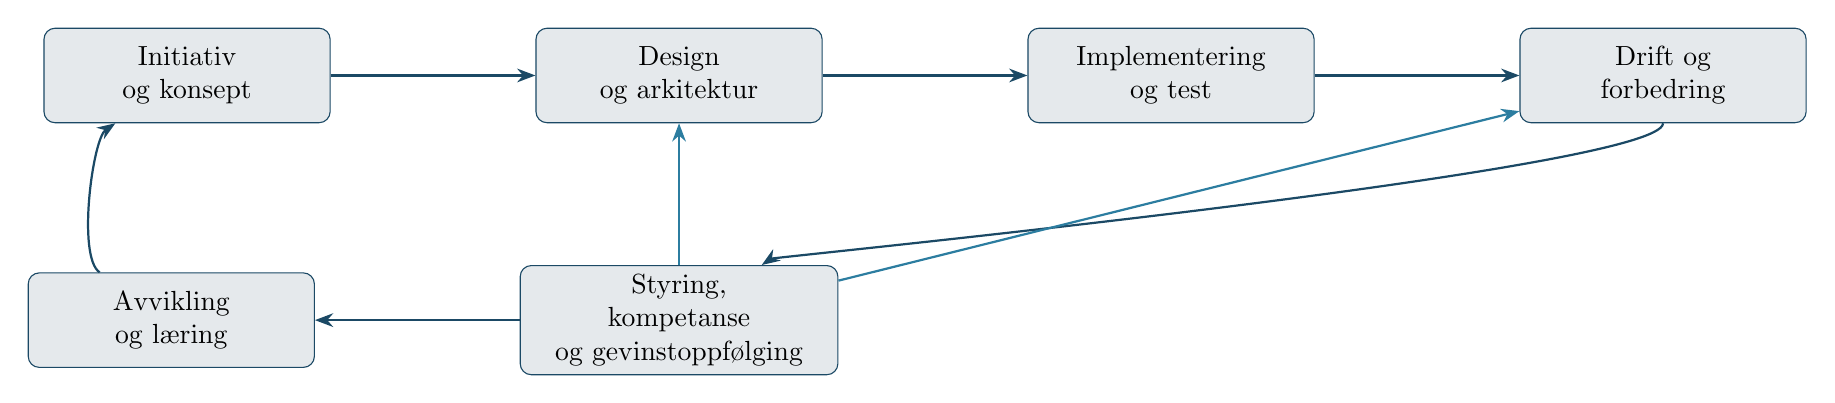
\begin{tikzpicture}[node distance=2.6cm, every node/.style={rectangle, rounded corners, draw=dypblaa, fill=skygraa, text width=3.4cm, align=center, minimum height=1.2cm}]
        \node (init) {Initiativ\\og konsept};
        \node[right=of init] (design) {Design\\og arkitektur};
        \node[right=of design] (implement) {Implementering\\og test};
        \node[right=of implement] (operate) {Drift og\\forbedring};
        \node[below=1.8cm of design, text width=3.8cm] (govern) {Styring,\\kompetanse\\og gevinstoppfølging};
        \node[left=of govern] (retire) {Avvikling\\og læring};
        \draw[->,>=Stealth,thick,dypblaa] (init) -- (design);
        \draw[->,>=Stealth,thick,dypblaa] (design) -- (implement);
        \draw[->,>=Stealth,thick,dypblaa] (implement) -- (operate);
        \draw[->,>=Stealth,thick,dypblaa] (operate) .. controls +(0,-1.2) and +(1.2,0.8) .. (govern);
        \draw[->,>=Stealth,thick,dypblaa] (govern) -- (retire);
        \draw[->,>=Stealth,thick,dypblaa] (retire) .. controls +(-1.2,0.8) and +(-1.2,-0.8) .. (init);
        \draw[->,>=Stealth,thick,petrol] (govern) -- (design);
        \draw[->,>=Stealth,thick,petrol] (govern) -- (operate);
    \end{tikzpicture}
    \caption{Livssyklusrammeverket som brukes i fagfelleløpet viser hvordan styring og læring kobles til fasene i \autoref{tab:raci-maritim}.}
    \label{fig:livssyklusramme}
\end{figure}

\section{Organisering og roller}
Styringen av digitale tvillinger krever en tydelig governance-modell som balanserer sentral koordinering og lokal innovasjon. Mange virksomheter etablerer et kjerneteam som forvalter plattformen, mens forretningsområder eller prosjektteam bygger spesifikke tvillinger på toppen.

\subsection*{Governance-modeller}
\begin{itemize}
    \item \textbf{Sentralisert modell:} Et dedikert «Center of Excellence» setter standarder, sikrer kompetanse og eier budsjett for tvillingplattformen. Passer godt i regulerte sektorer som energi og helse.
    \item \textbf{Føderert modell:} Domeneenheter eier sine tvillinger, men deler felles retningslinjer for data, sikkerhet og arkitektur. Et strategisk forum koordinerer veikart og prioriteringer.
    \item \textbf{Produktlinjemodell:} Tverrfaglige produktteam får ansvar for hele livssyklusen til en digital tvilling, inkludert finansiering og resultatmål. Plattformteam leverer felles komponenter og DevOps-støtte.
\end{itemize}

Tabell~\ref{tab:governance-sammenligning} sammenligner modellene på beslutningsfora, finansiering og egnethet. Oversikten brukes i workshops for å hjelpe virksomheter å vurdere hvilken struktur som passer deres modenhetsnivå.

\subsection*{Hybrid styring og utviklingssløyfer}
Selv om modellene beskrives separat, opplever mange virksomheter behov for en hybrid tilnærming. Et praktisk mønster er å etablere et sentralisert kjerneteam som definerer felles standarder, mens produktteam eier gevinstansvar. Det gir tre utviklingssløyfer som kan brukes i styringsdokumenter:
\begin{enumerate}
    \item \textbf{Strategisk sløyfe:} kvartalsvise portefølgemøter der konsernledelse, sikkerhetsansvarlige og produktteam samordner veikart og investeringer.
    \item \textbf{Taktisk sløyfe:} månedlige governance-forum der dataspace-råd, arkitektur og DevOps koordinerer endringsforslag og kvalitetskrav.
    \item \textbf{Operativ sløyfe:} ukevise standups med drift, domeneeksperter og læringsansvarlige som oppdaterer gevinstlogg og håndterer hendelser.
\end{enumerate}
Ved å tydeliggjøre hvilke beslutninger som tas i hver sløyfe, kan organisasjonen dokumentere ansvarslinjer i RACI-matrisen og justere ressursbehov etter modenhet.

\begin{table}[h]
    \centering
    \caption{Sammenligning av governance-modeller for digitale tvillinger}
    \label{tab:governance-sammenligning}
    \begin{tabular}{p{2.9cm}p{3.2cm}p{3.2cm}p{3.5cm}}
        \toprule
        Modell & Beslutningsfora & Finansiering & Typiske norske eksempler \\
        \midrule
        Sentralisert & Konsernråd for teknologi og sikkerhet & Sentralt investeringsbudsjett med felles gevinstplan & Statnetts nettplanleggingsprogram og Equinors Johan Sverdrup-plattform\citep{statnett2023digital,equinor2021johansverdrup} \\
        Føderert & Domenevise porteføljestyrer og dataspace-råd & Kostnadsdeling mellom virksomhetsområder etter bruk & Statsbyggs ombruksprogram og bytvillingen i Sluppen\citep{statsbygg2023loopfront,trondheim2024bytvilling} \\
        Produktlinje & Tverrfaglige produktteam med sprintdemoer & Produktteam eier resultatansvar, plattformteam fakturerer tjenester & Hydro CIRCALs materialsporingsprogram og Kognitwin-piloter i prosessindustri\citep{hydro2023traceability,kongsberg2023kognitwin} \\
        \bottomrule
    \end{tabular}
\end{table}

\subsection*{Rollefordeling og samhandling}
Produkteier, domeneekspert, data scientist, simuleringsspesialist og IT-drift må samarbeide tett. Rolleavklaringen bør konkretiseres gjennom en RACI-matrise som beskriver hvem som er ansvarlig (Responsible), beslutningstaker (Accountable), rådgiver (Consulted) og informert (Informed). Tabell~\ref{tab:raci-maritim} viser et eksempel for et maritimt vedlikeholdsprosjekt.

\begin{table}[h]
    \centering
    \caption{Eksempel på RACI-matrise for digital tvilling i maritimt vedlikehold}
    \label{tab:raci-maritim}
    \begin{tabular}{p{4cm}cccc}
        \toprule
        Aktivitet & Teknisk sjef & Produkteier & Data scientist & Skipsoffiser \\
        \midrule
        Definere vedlikeholdsstrategi & A & R & C & C \\
        Etablere datainnsamling & C & A & R & I \\
        Utvikle prediktiv modell & I & C & R & C \\
        Validere modell i drift & C & A & R & R \\
        Rapportere gevinster & R & A & C & I \\
        \bottomrule
    \end{tabular}
\end{table}

Eksterne leverandører bør inkluderes med klare kontrakter for ansvar og dataeierskap. Juridiske vurderinger må sikre at deling av sanntidsdata skjer i tråd med avtaler og regelverk.

\subsection*{RACI-variant for tverrsektorielle partnerskap}
Kryss-sektorielle initiativ, for eksempel batteriverdikjeder eller havvindplattformer, krever ofte at flere linjeorganisasjoner deler ansvar. En utvidet RACI-variant med kategorien \emph{Support} gjør det tydelig hvem som leverer operative ressurser selv om beslutningsmyndigheten ligger hos andre aktører. Tabell~\ref{tab:raci-variant} viser hvordan modellen kan anvendes på et dataspace-program der kommune, industri og teknologipartnere samarbeider.

\begin{table}[h]
    \centering
    \caption{RACI-S-matrise for dataspace-program i regionalt havvindinitiativ}
    \label{tab:raci-variant}
    \begin{tabular}{p{4.3cm}ccccc}
        \toprule
        Aktivitet & Kommune & Operatør & Plattformleverandør & Faglig rådgiver & TSO \\
        \midrule
        Fastsette delingspolicy og tilgangsnivå & A & C & R & C & I \\
        Implementere dataspace-kontrakter og API-er & I & C & R & C & S \\
        Overvåke datakvalitet og hendelser & C & R & S & C & A \\
        Planlegge vedlikeholdsvinduer & I & A & C & R & S \\
        Rapportere gevinster og bærekraftindikatorer & R & A & C & C & I \\
        \bottomrule
    \end{tabular}
\end{table}

Denne varianten forbereder leseren på å bruke malen i Appendiks~\ref{appendix:ressurser} der en generell tabell for RACI-S kan fylles ut for egne case.

\subsection*{Dataspace-governance og eskaleringslinjer}
Dataspace-samarbeid stiller krav til hvordan organisasjoner deler data, håndhever kontrakter og håndterer avvik. \citet{idsa2023ram} og \citet{gaiax2023architecture} beskriver hvordan noder må sertifiseres og hvordan tiltrode rollemyndigheter skal følge opp dataspace-policyer. Norske initiativ for mobilitet og energi legger til grunn at forvaltningsmodellen kombinerer tekniske komponenter (connectors, kataloger) med et styringsforum som kan sette bindinger for bruksvilkår.\citep{ec2023mobilitydataspace} For at kapittel 3 og 7 skal henge sammen i undervisningen, må studentene se hvordan dataspace-governance speiler de organisatoriske modellene over.

En praktisk måte å etablere styringen på er å definere fire beslutningsnivåer:
\begin{enumerate}
    \item \textbf{Strategisk råd:} Godkjenner dataspace-mandat, medlemskap og sanksjoner. Rådet eies gjerne av et offentlig-privat partnerskap hvor programleder for tvillinginitiativet sitter sammen med dataspace-operatør.
    \item \textbf{Operasjonelt forum:} Koordinerer onboarding, datakataloger og hendelser. Her deltar plattformteam, dataspace-arkitekter og juridiske rådgivere som vurderer datakontrakter mot \citet{digdir2023modelljournal}.
    \item \textbf{Domenegrupper:} Sektorspesifikke arbeidsgrupper (for eksempel helseteknologi eller mobilitet) som prioriterer data- og modellbehov, kvalitetssikrer semantikk og harmoniserer indikatorer fra Kapittel~6.
    \item \textbf{Eskaleringsteam:} Hurtigrespons-team med representanter fra sikkerhet, personvern og forretningssiden som kan pause deling eller oppdatere tilgangsvilkår ved avvik.
\end{enumerate}

Tabell~\ref{tab:dataspace-governance} viser hvordan styringsnivåene kan knyttes til konkrete artefakter og eskaleringspunkter i et regionalt dataspace-program. Oversikten kan brukes i casearbeid sammen med RACI-S-malen.

\begin{table}[h]
    \centering
    \caption{Styringsartefakter og eskalering i et regionalt dataspace-program}
    \label{tab:dataspace-governance}
    \begin{tabular}{p{3.2cm}p{4.2cm}p{4.2cm}p{3.0cm}}
        \toprule
        Beslutningsnivå & Hovedartefakt & Ansvarlige roller & Eskaleringspunkt \\
        \midrule
        Strategisk råd & Partnerskapsavtale med krav til sertifisering, medlemskap og gevinstplan & Programleder, kommuneadministrasjon, industripartnere & Revisjon mot dataspace-policy hvert halvår \\
        Operasjonelt forum & Datakatalog, tilgangspolicy og teknisk driftsrapport & Plattformteam, dataspace-arkitekt, juridisk rådgiver & Hendelser i connector eller uautorisert bruk \\
        Domenegrupper & Modelljournaler, semantiske vokabular og KPI-sett & Fagansvarlige, produktledere, data steward & Konflikt i datakvalitet eller indikatorer mellom sektorer \\
        Eskaleringsteam & Hendelseslogg, tilsynsrapport og beslutningslogg & Sikkerhetsleder, personvernombud, forretningsansvarlig & Pause eller stanse datadeling, varsling til tilsyn \citep{ec2023mobilitydataspace} \\
        \bottomrule
    \end{tabular}
\end{table}

Når artefaktene forvaltes i samme versjonskontroll som tvillingmodeller og datakataloger, blir det lettere å dokumentere etterlevelse av \citet{gaiax2023architecture} og å spore hvilke beslutninger som utløste endringer. Studentene bør kombinere tabellen med gevinstplanen under for å vise hvordan dataspace-governance støtter gevinstrealisering.

\subsection*{Gevinstplan og KPI-styring}
For å sikre kontinuerlig oppfølging bør kapittelteamet bruke en gevinstplan som kobler indikatorer til ansvarlige roller og beslutningsarenaer. Tabell~\ref{tab:gevinstplan} gir et eksempel på hvordan livssyklusfaser, KPI-er og datakilder kan organiseres. Malen speiler strukturen i Appendiks~\ref{appendix:ressurser} og kan tilpasses ulike sektorer.

\begin{table}[h]
    \centering
    \caption{Eksempel på gevinstplan for digital tvilling}
    \label{tab:gevinstplan}
    \begin{tabular}{p{2.8cm}p{3.8cm}p{3.5cm}p{3.2cm}}
        \toprule
        Livssyklusfase & Hovedindikator & Datakilde & Beslutningsarena \\
        \midrule
        Initiativ & Forventet netto nåverdi og modenhetsgrad & Forretningscase, vurderingsmatrise (Kapittel~8) & Porteføljestyre (kvartalsvis) \\
        Implementering & Sprintleveranser fullført og modellnøyaktighet & DevOps-rapporter, modellvalidering (Kapittel~6) & Styringsgruppe (hver sprint) \\
        Drift & Oppetid, datakvalitet og sikkerhetshendelser & Observabilitetsdashbord, hendelseslogger & Operasjonelt forum (ukentlig) \\
        Forbedring & Realiserte gevinster og læringspunkter & KPI-rapport, retrospektiver & Programstyre (månedlig) \\
        Avvikling & Dokumentert arv og gjenbruk & Arkiverte modeller, dataspace-policy & Kunnskapsforum (etterprosjekt) \\
        \bottomrule
    \end{tabular}
\end{table}

Ved å oppdatere gevinstplanen etter hver milepæl blir det lettere å holde oversikt over forutsetninger som må oppdateres når nye caser legges inn i undervisningen.

\subsection*{Bærekraft- og modenhetsindikatorer per sektor}
Livssyklusstyring må også følge opp klima- og ressursmål. Tabell~\ref{tab:baerekraft-kpi} gir eksempler på indikatorer fra tre sektorer som brukes i norske pilotprosjekter. De kompletterer gevinstplanen ved å vise hvordan bærekraftdata hentes og forankres i styringen.

\begin{table}[h]
    \centering
    \caption{Eksempler på bærekraft-KPI-er i norske digital-tvillingprosjekter}
    \label{tab:baerekraft-kpi}
    \begin{tabular}{p{2.9cm}p{3.6cm}p{3.2cm}p{3.3cm}}
        \toprule
        Sektor & Bærekraft-KPI & Datakilde & Formål \\
        \midrule
        Havvind & CO$_2$-intensitet per levert MWh og turbin-tilgjengelighet & Kombinerte driftssensorer og energibalanser fra Hywind Tampen & Dokumentere klimaeffekt og pålitelighet i samsvar med NVE-krav\citep{equinor2023hywindtampen,nve2023havvindfakta} \\
        Bygg og eiendom & Andel komponenter til gjenbruk samt avfallsreduksjon & BIM-modeller og Loopfront-logg for ombruk & Understøtte klimabudsjett og sirkulærøkonomistrategi hos Statsbygg\citep{statsbygg2023loopfront,regjeringen2021sirkulaer} \\
        Batteriverdikjede & Resirkuleringsgrad og energiforbruk per celle & Produksjonsdata fra Giga Arctic og leverandørsertifikater & Verifisere bærekraftskrav i støtteordninger og kundekontrakter\citep{freyr2024giga,enova2023batteri} \\
        \bottomrule
    \end{tabular}
\end{table}

Indikatorene brukes som utgangspunkt når studentene utvikler egne KPI-sett og kobler dem til dataspace-arkitekturen i \autoref{tab:governance-sammenligning}.

\subsection*{Modenhetssteg for bærekraftstyring}
For å knytte indikatorene til livssyklusen kan kapittelteamet bruke en trestegs modenhetsmodell. Den gjør det enklere å beskrive ambisjonsnivå i plan- og statusfiler og å følge opp tiltak i fagfellelogg:
\begin{enumerate}
    \item \textbf{Baseline:} Sektorteam registrerer grunnleggende klima- og ressursdata og kobler dem til ansvarlige roller i RACI-matrisen.
    \item \textbf{Integrert:} Bærekraft-KPI-er inngår i gevinstplan og beslutningsfora; dataspace-kontrakter sikrer deling med partnere.
    \item \textbf{Revisjonsklar:} Indikatorene revideres eksternt, støttes av sporbare dataprodukter og brukes i scenarioplanlegging for neste generasjon tvillinger.
\end{enumerate}
Modellen brukes som sjekkliste når nye case legges til i kapittel~\ref{chap:case} og når støttefilene oppdateres med krav til dokumentasjon.

\subsection*{Sirkulærøkonomisk gevinststyring}
Norske virksomheter forventes å dokumentere hvordan digitale tvillinger støtter ombruk, materialeffektivitet og klimaambisjoner.\citep{norskindustri2023sirkular,regjeringen2021sirkulaer} For å gjøre dette operativt bør gevinstplanen kobles til et sett med sirkulærøkonomiske indikatorer som følger tvillingen gjennom livssyklusen. Indikatorene må forankres i de samme beslutningsforaene som håndterer investeringer og dataspace-governance, slik at tiltakene prioriteres sammen med øvrige endringer.

Et praktisk oppsett for masterstudenter består av tre komponenter:
\begin{enumerate}
    \item \textbf{Material- og energiindikatorer:} Registrer gjenbrukbar andel, resirkuleringsgrad og energiforbruk per leveranse slik Statsbygg og Hydro gjør i sine tvillingprogram.\citep{statsbygg2022ombruk,hydro2023traceability}
    \item \textbf{Prosessindikatorer:} Følg opp hvor raskt komponenter flyttes gjennom sirkulære sløyfer og hvor mange beslutninger som er dokumentert i kontrolltårn eller fagfellelogg.
    \item \textbf{Resultatindikatorer:} Mål klimanytte, reduserte innkjøpskostnader og etterlevelse av offentlige krav, og del tallene i de samme gevinstmøtene som rapporterer økonomisk effekt.
\end{enumerate}

Tabell~\ref{tab:sirkular-livssyklus} viser hvordan indikatorene kan organiseres per fase og hvilke kilder som brukes. Strukturen speiler datastrømmene i kapittel~3 og gjør det tydelig hvem som eier målingene.

\begin{table}[h]
    \centering
    \caption{Sirkulærøkonomiske indikatorer gjennom livssyklusen}
    \label{tab:sirkular-livssyklus}
    \begin{tabular}{p{2.7cm}p{3.7cm}p{3.5cm}p{3.0cm}}
        \toprule
        Fase & Fokusområde & KPI og terskel & Datakilde/ansvar \\
        \midrule
        Initiativ & Sirkulær forretningscase & Potensiell ombruksandel $>30\%$ og CO$_2$-besparelse per år & Forretningsanalyse, livsløpsberegning (Kapittel~3) ledet av bærekraftsansvarlig \\
        Design & Material- og dataarkitektur & Fullstendig komponentregister og sporbarhetsplan & BIM/dataspace-kontrakter, modelljournal forvaltes av arkitekt \\
        Implementering & Operative sløyfer & Tid fra demontering til gjenbruk $<6$ uker, kvalitetssjekk i sandkasse & IoT-logger, kontrolltårnrapport (Kapittel~6) eid av operasjonsteam \\
        Drift & Kontinuerlig måling & Andel sirkulære leveranser per måned, energiforbruk per enhet & Observabilitetsdashbord og ERP-data, rapportert av produktteam \\
        Forbedring/avvikling & Læring og dokumentasjon & Dokumenterte læringspunkter og oppdaterte policyer innen 4 uker & Fagfellelogg, gevinstmøte og arkivansvarlig \\
        \bottomrule
    \end{tabular}
\end{table}

Når tabellen brukes i casearbeid, bør studentene samtidig oppdatere ressursbanken i appendikset med datasett og verktøy som støtter indikatorene. Dette sikrer at sirkulærøkonomi blir en integrert del av gevinststyringen og ikke et separat sideprosjekt.

\subsection*{Dataspace-arkitektur for styring og deling}
Livssyklusforvaltning i større økosystem krever en dataspace-arkitektur som definerer ansvar for dataprodukter, identitet og policy. En anbefalt struktur følger fire lag:
\begin{enumerate}
    \item \textbf{Dataprodukter og semantikk:} Domeneeiere beskriver datastrømmer med felles ordlister og metadata slik at partnere kan oppdage dem. Semantiske modeller gjør det mulig å koble tvillingen til dataspace-kontrakter.\citep{idsa2023ram}
    \item \textbf{Tillitstjenester:} Identitet, tilgangskontroll og policy-håndhevelse sørger for at bare autoriserte aktører får tilgang til sensitive data. Gaia-X nav og nasjonale forvaltere kan fungere som tillitsanker.\citep{gaiax2023architecture}
    \item \textbf{Edge og sky:} Data behandles så nær kilden som mulig for å sikre respons, mens aggregerte datasett lagres i sky for analyse og deling. Edge-noder må støtte samme sikkerhetskrav som sentrale plattformer.\citep{etsi2023mec}
    \item \textbf{Styringsfora:} Tverrfaglige råd følger opp avvik, oppdaterer gevinstplanen og prioriterer forbedringer. Output fra rådene dokumenteres i læringssløyfer (retrospektiver, fagfellelogg) slik at gevinstene kan revideres.
\end{enumerate}
Arkitekturen sikrer at gevinstplaner, RACI-matriser og modellforvaltning er koblet sammen gjennom felles dataprodukter og policyer.

\subsection*{Porteføljestyring og beslutningsporter}
Når flere digitale tvillinger inngår i samme program må ledelsen synliggjøre hvilke investeringer som gir størst effekt og når initiativ bør stoppes eller skaleres. En porteføljestyringsmodell samler gevinstplanen, dataspace-governance og læringssløyfene fra Kapittel~6 i et felles beslutningsforum.\citep{digdir2022gevinst,rcn2024digitalisering} Modellen gjør det mulig å prioritere mellom sektorer, balansere risiko og sikre at modne tvillinger får ressurser til videreutvikling.

Porteføljen styres gjennom fire hovedporter som dekker hele livssyklusen:
\begin{enumerate}
    \item \textbf{Port 0 – Idéutvelgelse:} vurderer strategisk verdi, data- og partnergrunnlag samt mulige koblinger til eksisterende dataspace-initiativ.
    \item \textbf{Port 1 – Pilotering:} beslutter finansiering av laboratorieløp og evaluerer regulatoriske forpliktelser før data deles.
    \item \textbf{Port 2 – Skalering:} kvalitetssikrer operasjonelle indikatorer, integrasjoner og gevinstplan før løsningen rulles ut bredt.
    \item \textbf{Port 3 – Drift og fornyelse:} følger opp realiserte gevinster, teknisk gjeld og beslutninger om videre investering eller avvikling.
\end{enumerate}

Tabell~\ref{tab:portefolje-porter} viser hvilke indikatorer og dokumenter som bør være klare ved hver port. Oversikten brukes i undervisningen for å koble fagteamene sine caseoppgaver til styringsarenaene i \autoref{tab:dataspace-governance} og gevinstplanen i Tabell~\ref{tab:gevinstplan}.

\begin{table}[h]
    \centering
    \caption{Beslutningsporter i porteføljen for digitale tvillingprogram}
    \label{tab:portefolje-porter}
    \begin{tabular}{p{2.8cm}p{3.8cm}p{3.4cm}p{3.4cm}}
        \toprule
        Port & Beslutningsfokus & Nøkkelindikatorer & Obligatoriske leveranser \\
        \midrule
        Port 0 – Idéutvelgelse & Strategisk relevans, datatilgang og partnerkapasitet & Forventet netto nytte, modenhetsanalyse og tilgangen til kritiske datasett & Hypotesekart, interessentoversikt og vurdering av dataspace-krav \\
        Port 1 – Pilotering & Gjennomføringskraft og regulatorisk klarering & Testplan, personvernrisiko og tilgangsklarering fra dataspace-forum & Laboratorieplan, sikkerhetsvurdering og beslutning om felles plattformressurser \\
        Port 2 – Skalering & Operasjonell robusthet og gevinstpotensial & Modellnøyaktighet, driftsindikatorer og gevinstplan med KPI-er & Integrasjonsarkitektur, kvalitetsjournal og oppdatert gevinstplan \\
        Port 3 – Drift og fornyelse & Gevinstrealisering, teknisk gjeld og videre investeringsbehov & Leveransegrad, revisjonsfunn og målt bærekraftseffekt & Oppdatert tiltakslogg, beslutning om videre finansiering og plan for neste iterasjon \\
        \bottomrule
    \end{tabular}
\end{table}

For kapittelteamet er porteføljestyringen en sjekkliste: Når en port er passert skal indikatorer og dokumenter oppdateres i planfilene og fagfelleloggen. Resultatene deles med programleder, slik at porteføljen rebalanseres i takt med nye case fra Kapittel~\ref{chap:case} og forskningsløpene i Kapittel~9.

\section{Endringsledelse og modenhet}
Digital tvilling er en organisasjonsutvikling like mye som et teknisk prosjekt. Modenhet kan vurderes i nivåer fra ad hoc-initiativ til kontinuerlig forbedring der tvillingen er integrert i virksomhetsstyringen. En modenhetsmodell kan beskrive kriterier for styringsstruktur, datakvalitet, automatisering og kompetanse på hvert nivå.

Endringsledelse handler om å bygge forståelse for hvorfor tvillingen er viktig, sikre eierskap hos ledelse og fagmiljø, og investere i opplæring. Kommunikasjon bør være målrettet mot ulike interessenter: operatører trenger praktiske arbeidsprosesser, mens ledelsen trenger indikatorer som viser strategisk effekt.

\subsection*{Måleindikatorer for gevinstrealisering}
Gevinster må følges opp med både kvantitative og kvalitative indikatorer:
\begin{itemize}
    \item \textbf{Operasjonelle KPI-er:} reduksjon i uplanlagt nedetid, optimalisert energiforbruk, forbedret produksjonsutnyttelse.
    \item \textbf{Kvalitetsindikatorer:} forbedret modellnøyaktighet, raskere saksbehandling for endringer, færre sikkerhetshendelser knyttet til datadelingsfeil.
    \item \textbf{Lærings- og innovasjonsmål (OKR-er):} antall eksperimenter kjørt i tvillingen per kvartal, nye tjenester som lanseres basert på innsikt fra tvillingen, kompetanseløft i tverrfaglige team.
\end{itemize}
Indikatorene bør inngå i virksomhetens styringssystem, eksempelvis balansert målstyring eller kvartalsvise portefølgereview. For å sikre kontinuerlig forbedring kan teamet gjennomføre retrospektiv-møter der avvik analyseres og tiltak prioriteres.

\subsection*{Kompetansepakke for dataspace-governance}
Fagfellepanelet etterspurte en helhetlig kompetansepakke som støtter dataspace-governance gjennom hele endringsreisen. Programlederen bør kombinere klasseromsøkter, digitale mikrokurs og praksisnære øvelser slik at både tekniske og organisatoriske roller får nødvendig trygghet. \citet{digdir2022gevinst} anbefaler at gevinstplan, organisering og kommunikasjon kobles til en egen opplæringsplan, mens \citet{dssc2023skills} beskriver hvordan dataspace-team må bygge kompetanse på både policy og teknologi. Tabell~\ref{tab:kompetansepakke} viser et opplegg som kan integreres i lærerveiledningen og caseøktene i Kapittel~\ref{chap:case}.

\begin{table}[h]
    \centering
    \caption{Kompetansepakke for dataspace-governance}
    \label{tab:kompetansepakke}
    \begin{tabular}{p{2.7cm}p{4.0cm}p{3.6cm}p{3.2cm}}
        \toprule
        Modul & Læringsmål & Nøkkelinnhold & Praktisk leveranse \\
        \midrule
        Strategisk oversikt & Forstå partnerskapsmodell, gevinstmål og regulatoriske krav & Dataspace-roller, gevinstplanlegging, kobling til NIS2 og personvern & Presentasjon og gevinstkart fra workshop \\
        Operasjonell forvaltning & Implementere policy, datakatalog og hendelseslogg & Modelljournal, tilgangsstyring, kontrolltårn-prosesser & Konfigurert mal i prosjektverktøy og oppdatert RACI-S \\
        Teknisk forankring & Beherske connector-arkitektur og kvalitetsmålinger & Referansearkitektur, testmiljø, observabilitetsdashbord & Proof-of-concept med integrert kvalitets- og sikkerhetsvarsling \\
        Endringsledelse og kommunikasjon & Planlegge opplæring, måleeffekter og forankre endringer & Målgruppetilpasning, kommunikasjonsplan, gevinstoppfølging & Kommunikasjonsplan og læringslogg delt i fagfelleloggen \\
        \bottomrule
    \end{tabular}
\end{table}

Kompetansepakken følger modenhetsstegene over og kan fases inn i pilotundervisningen uke~4--6. Studentene kan fordele modulene mellom roller i caset og bruke fagfelleloggen til å dokumentere hvem som trenger oppfølging.

\subsection*{Kommunikasjonsplan for endringsreise}
Effektiv endringsledelse krever målrettet kommunikasjon til ulike interessenter gjennom hele dataspace-reisen. Planen i Tabell~\ref{tab:kommunikasjonsplan} fungerer som sjekkliste i planleggingsfasen og kan justeres for sektorvise behov. Den kombinerer informasjonskanaler, ansvar og budskap slik \citet{digdir2022gevinst} anbefaler i gevinstoppfølgingen, og legger inn læringsaktiviteter i tråd med anbefalingene fra \citet{dssc2023skills} om kompetansebygging.

\begin{table}[h]
    \centering
    \caption{Kommunikasjonsplan for dataspace-endringsreise}
    \label{tab:kommunikasjonsplan}
    \begin{tabular}{p{2.8cm}p{3.6cm}p{3.6cm}p{3.4cm}}
        \toprule
        Fase & Målgrupper & Budskap og materiell & Ansvar og kanal \\
        \midrule
        Før oppstart & Programstyre, nøkkelpartnere, fagforeninger & Forretningsmål, gevinsthypoteser, forventet involvering & Programleder via styringsråd og partnerskapsbrev \\
        Pilotering & Operasjonsteam, dataspace-arkitekter, juridisk støtte & Policykrav, tilgangsprosesser, pilotcase og datakvalitetsmålinger & Dataspace-forum og dedikerte arbeidsmøter ledet av forvalter \\
        Utrulling & Sluttbrukere, leverandører, sikkerhetsmiljø & Endringsstøtte, opplæringstilbud, sikkerhetsrutiner og støttekanaler & Kommunikasjonsteam gjennom intranett, webinar og spørretimer \\
        Etterlevelse & Fagfeller, tilsyn, prosjektkontor & Resultater, gevinstrapport, læringslogg og videre tiltak & Programleder og fagteam gjennom kvartalsrapport og læringsworkshop \\
        \bottomrule
    \end{tabular}
\end{table}

Planen bør oppdateres etter hver retrospektiv. Studentteam kan bruke strukturen til å forberede interessentkart og identifisere hvor kommunikasjonsgap vil bremse gevinstrealiseringen.

\section{Intervjuguide for governance-case}
Tilbakemeldinger fra fagfellepanelet ba oss konkretisere hvordan intervjuer og workshops skal gjennomføres når governance-modellene testes i pilotundervisningen. Intervjuguiden i notatet `support/notater/pilotundervisning-materiell.md` brukes som grunnlag, og kobles til livssyklusfigur~\ref{fig:livssyklusramme} slik at hvert spørsmål peker til riktig fase og ansvar.

En strukturert økt kan gjennomføres slik:
\begin{enumerate}
    \item \textbf{Innledning (5 minutter):} Presenter formålet med caset og hvilke leveranser som skal testes. Bekreft samtykke til notater og eventuell opptak.
    \item \textbf{Fasevis dypdykk (20 minutter):} Bruk figuren til å kartlegge hendelser, beslutningspunkter og støtteverktøy i fasene initiativ, design, implementering og drift. Noter tydelige ansvar og avhengigheter.
    \item \textbf{Styring og gevinstoppfølging (10 minutter):} Undersøk hvordan indikatorer, opplæring og beslutningsfora fungerer i praksis. Diskuter hvordan tiltakene skal dokumenteres i fagfelleloggen.
    \item \textbf{Avslutning (5 minutter):} Oppsummer foreslåtte tiltak, avklar hvem som følger dem opp og hvilke data som kan deles videre i undervisningen.
\end{enumerate}

Resultatene bør overføres til fagfelleloggen og planens tiltaksoversikt slik at vi kan spore hvilke endringer som kreves før neste revisjon. Intervjuene danner også grunnlag for refleksjonsoppgaver i pilotundervisningen uke~5 og 6.

\section{Refleksjonsspørsmål og øvinger}
\begin{enumerate}
    \item Bruk Tabell~\ref{tab:raci-maritim} som inspirasjon og tilpass en RACI-matrise til et eget case, for eksempel en digital tvilling for kraftnett eller helseutstyr.
    \item Utform et sett med KPI-er og OKR-er som gjør det mulig å følge opp både kortsiktige driftsgevinster og langsiktig innovasjon.
    \item Beskriv hvilke tiltak som kreves for å løfte en organisasjon fra pilotnivå til helhetlig integrasjon av digitale tvillinger, inkludert styring, kompetanse og teknologi.
\end{enumerate}

\chapter{Bruksområder og norske case}

\section{Læringsmål}
\begin{itemize}
    \item Analysere variasjon i anvendelser av digitale tvillinger på tvers av sektorer.
    \item Kritisk evaluere norske case med hensyn til teknologi, organisasjon og gevinster.
    \item Overføre læring fra case til egne prosjekter.
\end{itemize}

\section{Industrisektoren}
Digitale tvillinger i norsk industri kobler ofte sammen komplekse produksjonslinjer, leverandørkjeder og energisystemer. Når du analyserer casene, bør du identifisere hvilke beslutningssituasjoner som styrer investeringen, og hvordan innsikten fra tvillingen brukes til både operativ og strategisk styring. Erfaringer fra Yara, Hydro og andre prosessaktører viser at kontinuerlig forbedring og vedlikehold er like sentralt som nye investeringer.

\subsection*{Prosessindustri og produksjon}
I ferrolegering, aluminium og batteriindustri ser vi digitale tvillinger som kombinerer sanntidsdata fra produksjonslinjene med simuleringer for å optimere varmebalanse, kjemiske prosesser og logistikk. Hydro Sunndal bruker for eksempel virtuelle modeller til å følge elektrolysecellene og planlegge vedlikehold før avvik oppstår. Ved å fylle ut casemalen kan du dokumentere hvordan datainnsamling fra sensorer, laboratorier og ERP-systemer kobles til modellene, og hvilke styringsparametre (for eksempel OEE og energibruk per enhet) som måles for å vise gevinst.

\subsection*{Energi og kraft}
Kraftbransjen kombinerer produksjonsdata, nettanalyser og markedssignaler for å sikre forsyningssikkerhet og bærekraft. Statnett utvikler digitale tvillinger av transmisjonsnettet for å planlegge vedlikehold og håndtere flaskehalser, mens Statkraft integrerer værdata og hydrologiske modeller for å optimalisere vannkraftmagasinene. Når du bruker malen på slike case, bør du beskrive hvordan datakilder som SCADA, værprognoser og regulatoriske krav påvirker modellene og beslutningsprosessene.

\subsection*{Maritim og offshore}
I maritim sektor kombinerer aktører som Equinor, Kongsberg Maritime og Ulstein simuleringer av skip og plattformer med sanntidsdata fra sensorer. Tvillingene brukes til å planlegge logistikk i Nordsjøen, forutse vedlikehold på subsea-utstyr og teste nye autonome funksjoner. Et godt utfylt case viser hvordan operasjonssentraler, kapteiner og tekniske team samarbeider rundt modellen, og hvordan tvillingen knyttes til sikkerhet og miljørapportering. Utforsk datakilder og planleggingsverktøy samlet i \autoref{sec:maritimressurser} for å beskrive logistikk, miljøforhold og regulatoriske krav i caseleveransene.

\paragraph{Autonome ferger i Trondheimsfjorden}
Pilotprosjektet rundt passasjerfergen \emph{Milliampere 2} demonstrerer hvordan autonome fartøy kan inngå i mobilitetsløsninger for norske byer og dokumenteres som en del av Trondheims satsing på nullutslippsmobilitet.\citep{ntnu2023milliampere2} FoU-programmet AutoFerry beskriver hvordan Zeabuz og forskningsmiljøene bygger tvillingen med modulære sensorer, simulatorer og styringssystemer som kan overføres til flere havner.\citep{sintef2024autoferry} Casebriefen i `support/notater/maritim-caseforberedelse.md` dokumenterer mål, datakilder og styringsstruktur og fungerer som startpunkt for å fylle casemalen. Oppgaven til studentene er å beskrive hvordan tvillingen binder sammen fartøyet, fjernoperatører og kommunens mobilitetsstyring, og hvilke regulatoriske rammer som gjelder for testtilatelser og beredskap.

\begin{itemize}
    \item Kartlegg sensorer og eksterne datakilder (MET-værdata, AIS-strømmer, havneinformasjon) og beskriv hvordan de strømmer inn i datasjøen og simulatorene.
    \item Forklar hvordan prosjektets governance fordeler ansvar mellom Zeabuz, Trondheim kommune og forskningspartnerne, og hvordan endringsrådet evaluerer nye autonome funksjoner.
    \item Definer KPI-er for punktlighet, energibruk og sikkerhetsrespons og knytt dem til læringsmålene i Kapittel~3 (dataflyt) og Kapittel~6 (tillit og etikk).
    \item Bruk vurderingsmatrisen i dette kapittelet til å sammenligne caset med andre maritime initiativer, og dokumenter funnene i fagfelleloggen slik at prioriteringen kan forankres.
\end{itemize}

Integrer gjerne en illustrasjon fra `support/illustrasjonsplan.md` som viser samspillet mellom fartøyet, fjernoperasjonssenteret og byens øvrige transportsystem. Dette gjør det lettere for lesere å forstå hvordan datastrømmene og beslutningssløyfene knyttes sammen i en urban, maritim kontekst.

\section{Prioriterte case for kommende fagfelleløp}
For å støtte fagfelleløpet prioriteres tre nye case som dekker norsk energiomlegging, grønn industri og landbruksmodernisering. Notatene i `support/notater/` utdyper datakilder, KPI-er og styringsmodeller slik at arbeidsgrupper kan forberede intervjuer og dokumentasjon.

\subsection*{Havvind – Sørlige Nordsjø II og Hywind Tampen}
Utbyggingen av flytende havvind gir et rikt læringsgrunnlag for digital tvilling. Statlige rammer for areal og nettilknytning kombineres med Equinors operasjonserfaring fra Hywind Tampen, der turbiner og kraftplattformer deler data for å balansere produksjon mot sokkelinstallasjoner.\citep{nve2023havvindfakta,equinor2023hywindtampen} Tvillingen må koordinere værprognoser, vedlikeholdslogistikk og energioppgjør i en delt dataspace mellom operatør, Statnett og tjenesteleverandører.

\subsection*{Landbruk – Presisjonsjordbruk i Trøndelag}
Presisjonsjordbruket gir studentene innsikt i kombinasjonen av edge-prosessering og sentral analyse. Jord- og maskinsensorer prosesseres lokalt for å støtte autonome arbeidsoperasjoner, mens agronomiske beslutninger dokumenteres i felles datasett for rådgivere og forvaltning.\citep{nibio2023dataflyt,landbruksdir2023digitalisering,etsi2023mec} Caset viser hvordan data kan deles mellom gårdbruker, forskningsmiljø og kooperativ med klare policyer for gjenbruk av feltdata.

\subsection*{Batteriverdikjede – Giga Arctic i Mo i Rana}
Norsk batteriproduksjon kobler prosessindustri, energi og logistikk. FREYR Battery etablerer digitale tvillinger som følger råvarer, produksjonslinjer og energiforbruk for å oppfylle kravene i EUs batteriforordning og Enovas støtteordninger.\citep{freyr2024giga,enova2023batteri,gaiax2023architecture} Dataspace-tilnærmingen gjør at leverandørkjeder kan dele karbondata og kvalitetsmålinger under strenge kontraktsregimer.

\begin{table}[h]
    \centering
    \caption{Oversikt over prioriterte case og nøkkelindikatorer}
    \label{tab:prioriterte-case}
    \begin{tabular}{p{3.2cm}p{2.6cm}p{4.6cm}p{3.6cm}}
        \toprule
        Case & Sektor & Hovedindikatorer & Dataspace-fokus \\
        \midrule
        Sørlige Nordsjø II / Hywind Tampen & Havvind & Kapasitetsfaktor, planlagt vs. faktisk vedlikehold, HSE-observasjoner & Deling av produksjons- og værdata mellom operatør, TSO og offshore-partnere \\
        Presisjonsjordbruk i Trøndelag & Landbruk & Avlingsprognose, nitrogenutnyttelse, klimafotavtrykk per enhet & Samtykkebasert deling av feltdata og agronomiske anbefalinger mellom bønder og rådgivere \\
        Giga Arctic, Mo i Rana & Batteri & First-pass yield, energiforbruk per GWh, CO$_2$-intensitet per celle & Kontraktsstyrt tilgang til prosess-, logistikk- og bærekraftsdata i industrielt dataspace \\
        \bottomrule
    \end{tabular}
\end{table}

Casebeskrivelsene bygger videre på casemalen i dette kapittelet og gevinstplanen i Kapittel~7. Sektorgruppene bør fylle ut notatmalene med intervjuer, datatilgang og planlagte figurer før fagfellemøtene.

\subsection*{Dataspace-arkitektur for sektorkase}
Casene over illustrerer hvordan dataspace-prinsipper kan gjøre deling tryggere og mer fleksibel. Start med å etablere dataprodukter (for eksempel værvinduer, gjødselplaner eller energirapporter) med tydelig lisens. Bruk standardiserte policy-rammeverk fra IDSA og Gaia-X for å modellere tilgang og forretningsregler, og koble dem til KPI-oppfølgingen.\citep{idsa2023ram,gaiax2023architecture} Resultatet dokumenteres i prosjektets gevinstplan og RACI-matriser, slik at undervisningscasene får en konsistent styringsstruktur.

\section{Bygg, transport og helse}
Offentlige og private aktører bruker digitale tvillinger til å koordinere investeringer og tjenester som påvirker hele samfunnet. Felles utfordringer er å forankre tvillingen i eksisterende forvaltningssystemer, sikre datadeling og bygge kompetanse på tvers av fagmiljøer. Casemalen hjelper deg med å tydeliggjøre roller og datakilder i prosjekter der mange interessenter må samarbeide.

\subsection*{Smarte bygg og byer}
Statsbygg, Oslo kommune og flere norske byer har tatt i bruk digitale modeller som kombinerer BIM-data med energi- og sensorinformasjon for å styre drift og vedlikehold. Ved å beskrive scope, datakilder og governance i casemalen kan du vise hvordan driftsteam, leietakere og tjenesteleverandører bruker tvillingen til å redusere energibruk, planlegge renhold og forbedre inneklima.

\subsection*{Transport og logistikk}
Bane NOR utvikler digitale tvillinger av jernbanenettet for å planlegge vedlikehold, simulere trafikkavvik og informere kundeservice. Avinor tester tilsvarende modeller på flyplasser for å koordinere bakketjenester. Når du analyserer slike case, må du kartlegge hvordan sanntidsdata fra sensorer, IoT-enheter og trafikkstyringssystemer flyter inn i tvillingen, og hvordan det støtter planlegging og krisehåndtering. Utforsk datakilder som Entur, Bane NOR og Avinor i \autoref{sec:transportressurser} for å sikre at caserapporter støttes av konkrete tidsserier, kapasitetsdata og hendelseslogger.

\subsection*{Helse}
Helse Vest og Universitetssykehuset i Oslo eksperimenterer med pasientspesifikke tvillinger for kreftbehandling, kirurgisk planlegging og rehabilitering. Malen gir struktur for å beskrive hvordan kliniske data, bildediagnostikk og simuleringer integreres, hvilke etiske vurderinger som gjøres, og hvordan pasienter og fagpersonell involveres i beslutninger.

\section{Metodikk for caseanalyse}
For å sammenligne case på tvers av sektorer, start med å beskrive hvorfor tvillingen ble etablert, hvilke forutsetninger som må være til stede og hvordan resultatene måles. Det kan være nyttig å kombinere casemalen med intervjuer, offentlige rapporter og tekniske arkitekturdokumenter. Et helhetlig rammeverk bør dekke mål, omfang, teknologivalg, organisering og dokumenterte effekter.

\begin{itemize}
    \item Kartlegg datakilder systematisk, fra sanntidssensorer til historiske arkiv og åpne data, og vurder kvalitet, eierskap og tilgang.
    \item Noter hvilke styringsstrukturer, insentiver og kompetanseprogram som påvirker gjennomføring og skalering.
    \item Reflekter over etiske og samfunnsmessige hensyn, inkludert personvern, arbeidstakerperspektiv og miljøpåvirkning.
\end{itemize}

\subsection*{Vurderingsmatrise for modenhet og prioritering}
Når flere potensielle case konkurrerer om oppmerksomhet eller undervisningsressurser, kan en vurderingsmatrise gi et felles
beslutningsgrunnlag. Tabellen under brukes til å skåre hvert case fra~1 (lav modenhet) til~5 (høy modenhet) på fem dimensjoner.
Noter begrunnelsen for hver skår og lenk til dokumentasjon, slik at fagfeller kan etterprøve vurderingen.

\begin{longtable}{p{0.23\textwidth}p{0.26\textwidth}p{0.45\textwidth}}
\toprule
\textbf{Kriterium} & \textbf{Hva vurderes?} & \textbf{Eksempel på skåringsskala (1--5)} \\
\midrule
\endfirsthead
\toprule
\textbf{Kriterium} & \textbf{Hva vurderes?} & \textbf{Eksempel på skåringsskala (1--5)} \\
\midrule
\endhead
Datagrunnlag og tilgang & Tilgjengelighet, kvalitet og rettigheter til data som trengs for tvillingen. & 1~= fragmenterte kilder uten tilgangsavklaringer. 3~= etablerte datastrømmer, men mangler kvalitetssikring. 5~= sanntidsdata med avtalte API-er, eierskap og datakvalitetsrutiner. \\
\addlinespace
Organisatorisk forankring & Hvor godt case er støttet av ledelse, fagmiljø og brukere. & 1~= initiativ fra enkeltperson uten mandat. 3~= prosjektgruppe med midlertidig finansiering. 5~= tverrfaglig styringsmodell med dedikerte roller og gevinstansvar. \\
\addlinespace
Teknologisk modenhet & Modenhet på modeller, integrasjonsplattform og driftsoppsett. & 1~= konseptskisse uten implementert plattform. 3~= pilot i begrenset produksjon. 5~= robust løsning med DevOps-/MLOps-sløyfer og overvåkning i drift. \\
\addlinespace
Gevinst- og læringspotensial & Forventet effekt for virksomheten og læringsverdi for studenter. & 1~= uklare mål og lite overføringsverdi. 3~= tydelige KPI-er, men begrenset dokumentasjon. 5~= målbare gevinster, åpne data/artefakter og tydelig kobling til læringsmål. \\
\addlinespace
Risiko og etterlevelse & Regulatoriske, sikkerhets- og etiske forutsetninger. & 1~= ukjente krav eller høy personvernrisiko. 3~= identifiserte tiltak, men ufullstendig dokumentasjon. 5~= komplette risikovurderinger, etterlevelsesplan og jevnlig revisjon. \\
\bottomrule
\end{longtable}

Etter at tabellen er fylt ut, summeres skårene for et samlet modenhetsnivå, men noter også hvordan svakheter skal håndteres.
Følg denne arbeidsflyten for å forankre prioriteringen:

\begin{enumerate}
    \item Sett sammen et tverrfaglig vurderingsteam (for eksempel produktansvarlig, dataarkitekt og domeneekspert) og avklar
    hva slags beslutning som skal tas.
    \item Innhent nødvendig dokumentasjon: prosjektmandat, tekniske beskrivelser, datalister og gevinstrealiseringsplaner. Bruk
    ressursoversikten i \autoref{appendix:ressurser} for å finne støttedata eller verktøy som mangler.
    \item Skår casene i fellesskap, dokumenter begrunnelser og registrer resultatet i prosjektets styrings- eller fagfellelogg.
    \item Definer tiltak for kriterier som får skår 1--2 (for eksempel avklare tilgang, etablere governance eller komplettere
    risikovurdering) og gi tydelig anbefaling om case skal prioriteres, videreutvikles eller settes på vent.
\end{enumerate}

Ved å dele vurderingsmatrisen med studenter og eksterne samarbeidspartnere blir det lettere å diskutere hvilke case som gir mest
verdi, og hvilke forberedelser som kreves før data kan deles eller modeller kobles på.

\section{Casestudie-mal: Digital tvilling for batteriproduksjon i Mo i Rana}
Denne malen er inspirert av etableringen av den nasjonale batteriverdikjeden i Mo i Rana, der en digital tvilling skal binde sammen prosesslinjer, energiforbruk og logistikk. Bruk strukturen nedenfor som ramme for å dokumentere og analysere egne case, og erstatt eksemplene med data fra den faktiske virksomheten du studerer.

\subsection{Sammendrag av caset}
\begin{tabular}{p{0.32\textwidth}p{0.62\textwidth}}
\textbf{Element} & \textbf{Beskrivelse / spørsmål som skal besvares} \\
Virksomhet og lokasjon & Hvilken organisasjon studeres, og hvor er den plassert? \\
Strategisk hovedmål & Hva ønsker virksomheten å oppnå med den digitale tvillingen (for eksempel redusert energibruk eller økt kapasitet)? \\
Scope for tvillingen & Hvilke deler av verdikjeden eller prosesslinjen inngår? \\
Status ved prosjektstart & Hvilke systemer, datakilder og arbeidsprosesser fantes fra før? \\
\end{tabular}

\subsection{Forretningsmål og interessenter}
\begin{itemize}
    \item Beskriv konkrete forretningsmål og prioriteringer (for eksempel energieffektivitet, kvalitetskontroll eller fleksibel skalering).
    \item Identifiser hovedinteressenter: produksjonsledelse, operatører, IT/OT-team, energiselskap, logistikkpartnere og lokale myndigheter.
    \item Avklar hvordan målene måles, inkludert KPI-er som OEE, energiforbruk per battericelle og skraprate.
\end{itemize}

\subsection{Datagrunnlag og integrasjon}
\begin{itemize}
    \item Kartlegg hvilke datastrømmer som trengs: sensorer langs elektrodefabrikasjonen, MES/ERP-data, vær- og strømpriser, lager- og transportstatus.
    \item Vurder kvalitet, oppdateringsfrekvens og eierskap til hver datakilde.
    \item Beskriv integrasjonsarkitekturen, for eksempel OPC UA mot produksjonsutstyr og skybasert datasjø for historiske data.
\end{itemize}

\subsection{Modelleringsstrategi}
\begin{itemize}
    \item Definer hvilke modelltyper som skal inngå: prosessimulering, energimodell, logistikkmodell og prediktive vedlikeholdsmodeller.
    \item Spesifiser modelloppløsning (granularitet), valideringsdata og hvordan modeller kalibreres mot observasjoner.
    \item Marker antatte begrensninger eller usikkerheter, som begrenset historikk fra nyetablert produksjon.
\end{itemize}

\subsection{Implementering og arbeidsprosesser}
\begin{itemize}
    \item Beskriv hvordan tvillingen tas i bruk i daglig drift: dashboards i kontrollrom, digitale arbeidsordre, simulering før omstilling.
    \item Legg inn plan for opplæring av operatører og samarbeid mellom dataanalytikere og prosessingeniører.
    \item Dokumenter forvaltningsmodell: hvem eier modellen, hvordan versjoneres den, og hvordan sikres datakvalitet over tid?
\end{itemize}

\subsection{Resultater, gevinster og gevinstrealisering}
\begin{itemize}
    \item Oppgi konkrete gevinster som måles, for eksempel 8~\% lavere energiforbruk, redusert kassasjon eller raskere oppskalering av nye produktserier.
    \item Beskriv metoder for å verifisere gevinster, inkludert før- og etter-målinger og kontrollgrupper.
    \item Noter sekundære effekter: bedre HMS-oppfølging, samarbeid med kraftleverandør eller nye forretningsmodeller.
\end{itemize}

\subsection{Overføringsverdi og neste steg}
\begin{itemize}
    \item Drøft hvilke komponenter som kan gjenbrukes i andre norske industrier, for eksempel prosessmodeller, datastrømsarkitektur eller governance.
    \item Identifiser videre utvikling: kobling mot leverandørkjede, bruk av AI til kvalitetssikring, integrasjon med europeiske energimarkeder.
    \item Foreslå indikatorer og beslutningspunkter for å evaluere når tvillingen bør oppdateres eller skaleres.
\end{itemize}

\subsection*{Sjekkliste for caserapporten}
\begin{itemize}
    \item[$\square$] Har du dokumentert mål, interessenter og scope?
    \item[$\square$] Er alle relevante datakilder og integrasjoner beskrevet?
    \item[$\square$] Inneholder rapporten tydelige modelleringsvalg og begrunnelser?
    \item[$\square$] Er det lagt inn plan for drift, opplæring og governance?
    \item[$\square$] Er gevinstene målbare og knyttet til KPI-er som følges opp?
    \item[$\square$] Er læringspunkter og videre tiltak formulert?
\end{itemize}

\subsection{Eksempler på norske casetilpasninger}
\paragraph{Digital tvilling av kraftnett i Nord-Norge}
Statnett og regionale nettselskaper samarbeider om å modellere flaskehalser i kraftnettet mellom Ofoten og Finnmark. Når casemalen brukes på dette prosjektet, bør du beskrive hvordan værdata, planlagte industrietableringer og driftsmønstre fra vann- og vindkraft integreres. Vurder også hvordan tvillingen støtter dialogen med NVE og lokalsamfunn.

\paragraph{Jernbanedrift og vedlikehold hos Bane NOR}
En digital tvilling av jernbanestrekningen mellom Oslo og Lillehammer kombinerer BIM-modeller, sensordata fra spor og sanntidssignaler fra togene. Ved å følge malen kan du dokumentere hvordan operasjonssentralen, entreprenører og leverandører samarbeider om vedlikeholdsvinduer, og hvordan simuleringer brukes til å planlegge nye ruteoppsett.

\paragraph{Virtuell pasientflyt i spesialisthelsetjenesten}
Helse Sør-Øst prøver ut digitale tvillinger for å koordinere pasientflyt i kreftbehandling. Malen hjelper deg å tydeliggjøre hvilke kliniske datasett som inngår, hvordan algoritmer foreslår behandlingsplaner og hvordan pasienter får informasjon. Etisk vurdering, datasikkerhet og samtykkeprosesser må dokumenteres grundig.

\section{Refleksjonsspørsmål og øvinger}
\begin{enumerate}
    \item \textbf{Analyse av eksisterende case:} Velg ett av caseeksemplene ovenfor eller et eget norsk prosjekt. Bruk casemalen til å skrive en kort rapport (2--3 sider) der du vurderer modenhet, måloppnåelse og hvilke ytterligere datakilder som kan styrke tvillingen.
    \item \textbf{Planlegging av nytt initiativ:} Sett sammen et tverrfaglig team (for eksempel prosessingeniør, data scientist og driftsleder) og lag et arbeidsnotat som beskriver hvordan dere vil samle data, utvikle modeller og organisere forvaltning for et nytt case i deres sektor.
    \item \textbf{Tverrsektoriell overføring:} Sammenlign to sektorer, for eksempel kraft og bygg. Lag en tabell som viser hvilke komponenter i casemalen som er direkte overførbare, hvilke som må tilpasses, og foreslå tiltak for å gjenbruke modeller eller datagrunnlag.
    \item \textbf{Refleksjon over etikk og verdiskaping:} Diskuter i grupper hvordan personvern, arbeidsmiljø og bærekraft bør ivaretas når tvillinger skaleres. Bruk notater fra de tre foregående oppgavene og oppdater casemalen med konkrete risikoreduserende tiltak.
\end{enumerate}

\chapter{Fremtidstrender og forskning}

\section{Læringsmål}
\begin{itemize}
    \item Identifisere forskningsfronten innen digitale tvillinger.
    \item Diskutere fremtidige teknologier og samfunnsmessige konsekvenser.
    \item Formulere forskningsspørsmål og prosjektidéer.
\end{itemize}

\section{Forskningslandskapet}
Digitale tvillinger har etablert seg som et tverrfaglig forskningsfelt der systemteknikk, informatikk og domeneekspertise møtes. De mest synlige trendene springer ut av store internasjonale programmer som kobler akademia, leverandørindustri og offentlige aktører, samtidig som nasjonale prioriteringer legger føringer for hvilke problemstillinger som løftes frem i Norge.

\subsection{Internasjonale drivere}
EU har gjort digitale tvillinger til et kjerneelement i \emph{Horizon Europe} gjennom klynger som fokuserer på industriell digitalisering, energi og helseteknologi. Programmer som \emph{Destination Earth} og Gaia-X arbeider med felles dataplattformer og modeller for kritisk infrastruktur, og setter standarder som også påvirker norske miljøer. På forskningssiden markerer IEEE, ISO og Plattform Industrie 4.0 seg med veikart for interoperabilitet, semantikk og sikkerhet. Det gir en rik portefølje av referansemodeller, åpne datasett og calls for proposals som masterstudenter kan bruke som utgangspunkt for problemstillinger.

\subsection{Norske satsinger}
Forskningsrådet finansierer flere store miljøer, blant annet SFI Manufacturing, SFI Autoship og FME Neutron som alle utforsker digitale tvillinger i produksjon, maritime operasjoner og energi. Disse prosjektene kombinerer laboratorier, pilotanlegg og partnerskap med selskaper som Equinor, Kongsberg Gruppen, Elkem og offentlige etater. I tillegg gir regionale initiativ som katapultsentrene og Grønn plattform-prosjekter tilgang til testfasiliteter for masterstudenter. Norske kommuner og helseregioner stiller etter hvert krav om digitale tvillinger i anskaffelser, noe som åpner dører for anvendt forskning på mobilitet, helse og byggforvaltning.

\subsection{Samarbeidsformer og metoder}
Feltet domineres av tverrfaglige metoder som kobler modellering, dataanalyse og brukerinnsikt. Levende laboratorier (living labs) og sandkasser gjør det mulig å eksperimentere med datatilgang, mens dataspaces og standardiserte API-er legger til rette for datadeling på tvers av virksomheter. Publikasjoner i tidsskrifter som \emph{Computers in Industry}, \emph{Advanced Engineering Informatics} og \emph{IEEE Access} viser en utvikling fra konseptstudier til empiriske evalueringer av driftseffekter og bærekraftsgevinster. En masterstudent bør derfor kombinere kvantitative indikatorer (for eksempel energi, kvalitet eller risiko) med kvalitative intervjuer som belyser organisering og beslutninger.

\section{Teknologitrender}
Teknologisk utvikling setter nye rammer for hva digitale tvillinger kan løse og hvordan de driftes. Det skjer en sammensmelting mellom simuleringsverdenen, sanntidsdata og intelligent beslutningsstøtte, noe som øker autonomien i både industrielle og samfunnsrettede systemer.

\subsection{Generativ AI og beslutningsassistenter}
Foundation-modeller og multimodale generative teknikker brukes nå til å foreslå designalternativer, generere syntetiske datasett og veilede operatører i komplekse beslutninger. Industripartnere eksperimenterer med copiloter som kombinerer naturlig språk, visualisering og historiske tvillingdata for å foreslå tiltak i sanntid.\citep{siemens2023copilot} Den europeiske AI-handlingsplanen fremhever behovet for ansvarlige, dokumenterte modeller, noe som innebærer at tvillinger må ha forklaringslag og revisjonsspor før generativ AI kan tas i bruk i regulerte bransjer.\citep{eu2023ai}

\subsection{Edge-native tvillinger}
For prosesser som krever lav responstid kombineres digitale tvillinger med edge-komponenter der databehandling skjer tett på utstyret. Standarder for multi-access edge computing gjør det mulig å orkestrere containere og AI-modeller i fabrikkhaller, på fartøy eller i landbruksmaskiner, samtidig som policyer for dataspace-tilgang ivaretas.\citep{etsi2023mec} Edge-native mønstre utfordrer tradisjonell skyarkitektur og krever at DevOps- og MLOps-prosesser inkluderer distribuerte oppdateringer, overvåking og fallback-rutiner.

\subsection{Semantiske tvillinger og autonomi}
De mest modne tvillingene bygger nå på semantiske modeller der kunnskapsgrafer og ontologier beskriver forholdet mellom komponenter, datastrømmer og forretningsregler. Kombinert med maskinlæring, probabilistiske modeller og formelle verifikasjonsmetoder gir dette grunnlag for beslutninger som kan automatiseres. Autonome tvillinger brukes til å orkestrere vedlikehold, balansere energinett og styre logistikksystemer, men krever transparens og sporbarhet slik at operatører kan forstå og overstyre kritiske valg.

\subsection{Immersive arbeidsflater og metaverset}
Utvidet virkelighet, digitale arbeidsrom og metaverse-plattformer gjør det mulig å visualisere komplekse systemer for operatører og borgere. Kombinasjonen av 3D-modeller, sanntidsstrømmer og samarbeidsverktøy lar tverrfaglige team samhandle om scenarioanalyse, opplæring og fjernoperasjon. Forskningen fokuserer på hvordan slike grensesnitt kan gi situasjonsforståelse uten å overbelaste brukeren, og hvordan sikkerhet og personvern ivaretas når data distribueres til mange enheter.

\subsection{Bærekraft og regulering}
\subsection{Dataspace-økosystemer og samarbeid}
Europeiske dataspace-initiativer endrer hvordan virksomheter deler data og modeller. Gaia-X og IDSA legger til rette for at digitale tvillinger kan kobles på eksterne datastrømmer uten å gi fra seg kontroll over forretningshemmeligheter.\citep{gaiax2022architecture} For norske aktører betyr dette at energidata, maritime logistikkstrømmer eller helseinformasjon kan tilgjengeliggjøres gjennom standardiserte konnektorer, samtidig som tilgang styrt av policyer og sertifisering. Forskningsfronten ser på hvordan slike dataspace-plattformer kan kombineres med semantiske modeller og automatisert etterlevelse, slik at tvillinger kan forhandle om datadeling i sanntid og dokumentere hvilke regler som gjelder for hver transaksjon.

Masterprosjekter og pilotundervisningen bør derfor undersøke dataspace-strategier tidlig: avklar hvilke delingsnoder som finnes i sektoren, hvilke tilganger som krever godkjenning, og hvordan tvillingen håndterer logging og audit når data flyttes mellom organisasjoner. Dette gir også mulighet for komparative studier av hvordan ulike dataspace-implementeringer støtter NIS2 og andre sikkerhetskrav.

Digitaliseringsstrategier forventes å dokumentere klima- og ressursgevinster, og digitale tvillinger brukes som beslutningsgrunnlag for grønn omstilling. Forskningen undersøker hvordan tvillingene kan kobles til EU-taksonomien, rapportere Scope 1–3 utslipp og støtte sirkulærøkonomiske modeller. Dette stiller krav til datakvalitet, revisjonsspor og etterlevelse av regelverk som NIS2 og personvernforordningen, samtidig som det åpner for nye tjenester knyttet til sertifisering og revisjon.
\subsection{Bærekraft, dataspace og regulering}
Digitaliseringsstrategier forventes å dokumentere klima- og ressursgevinster, og digitale tvillinger brukes som beslutningsgrunnlag for grønn omstilling. Forskningen undersøker hvordan tvillingene kan kobles til EU-taksonomien, rapportere Scope 1–3 utslipp og støtte sirkulærøkonomiske modeller. Dataspace-initiativer i transport og energi legger føringer for hvordan dataprodukter beskrives, lisensieres og revideres, og gjør det enklere å dele gevinster på tvers av aktører.\citep{ec2023mobilitydataspace,idsa2023ram} Dette stiller krav til datakvalitet, revisjonsspor og etterlevelse av regelverk som NIS2 og personvernforordningen, samtidig som det åpner for nye tjenester knyttet til sertifisering og revisjon.

\section{Fra idé til prosjekt}
Å utvikle en masteroppgave eller et forskningsprosjekt innen digitale tvillinger innebærer å knytte tekniske muligheter til et meningsfullt problem i en valgt sektor. Prosessen starter med å forstå eksisterende praksis, avdekke kunnskapshull og sette mål som kan måles.

\subsection{Identifisere forskningshull}
Begynn med en systematisk litteraturgjennomgang i databaser som Scopus og Oria, og kartlegg hvilke prosesser, teknologier eller brukergrupper som er lite omtalt. Sammenlign funnene med behov fra industripartnere eller offentlige virksomheter. Gap analyseres ofte i grensesnittet mellom teknologi og organisasjon: Hvordan påvirker nye datakilder beslutninger, hvilke barrierer finnes for deling, og hvilke usikkerheter må håndteres?

\subsection{Metodevalg og datainnsamling}
Valg av metode bør speile både teknologiens modenhet og tilgjengelige ressurser. Eksperimentelle design kan brukes når man har tilgang til laboratorier eller simuleringsmiljøer, mens casestudier gir verdi når feltdata må samles i samarbeid med virksomheter. Mixed-methods med både kvantitative målinger og kvalitative intervjuer blir stadig vanligere for å dokumentere effekter og endringsledelse. Masterstudenter bør tidlig avklare datatilgang, lisensbehov og etiske avklaringer (for eksempel REK eller NSD) slik at prosjektet blir gjennomførbart.

\subsection*{Indikatorer for forskningsfremdrift}
Fagfelleløp og masterprosjekter kan bruke indikatorene i Tabell~\ref{tab:forskningsindikatorer} for å holde fremdrift og datasamarbeid under kontroll. Indikatorene er hentet fra porteføljestyring i norsk forskningsfinansiering og kobler resultater til samarbeid i dataspace.

\begin{table}[h]
    \centering
    \caption{Forslag til KPI-er for forsknings- og innovasjonsprosjekter}
    \label{tab:forskningsindikatorer}
    \begin{tabular}{p{2.6cm}p{3.8cm}p{3.8cm}p{3.2cm}}
        \toprule
        Fase & KPI & Beskrivelse & Datakilde \\
        \midrule
        Problemforståelse & Andel kartlagte datasett og partnere & Deling av metadatakort i dataspace-katalog & Prosjektlogg, dataspace-dashboard \\
        Metodeutvikling & Andel eksperimenter med reproduserbare skript & Kode- og modellpakker publisert med versjonering & Git-repositorier, laboratorienotat \\
        Evaluering & Dokumenterte effekter (for eksempel energi, kvalitet, sikkerhet) & Sammenligning av før/etter-KPI-er og fagfelleuttalelser & Evalueringsrapporter, gevinstplan \\
        Formidling & Antall åpne dataprodukter eller artikler & Publisering i kanaler definert av finansieringsprogram & Publiseringsdatabase, dataspace-katalog \\
        Videreføring & Finansiert oppskalering eller pilot & Nye kontrakter, videre forskningsmidler & Prosjektregnskap, Forskningsrådets porteføljerapporter \\
        \bottomrule
    \end{tabular}
\end{table}

Indikatorene støtter kravene i porteføljeanalysen for digitalisering og muliggjør datadeling gjennom standardiserte policyer og kontrakter.\citep{rcn2024digitalisering}

\subsection{Publisering og nettverk}
Planlegg formidling parallelt med forskningen. Målrett konferanser som \emph{Model-Based Systems Engineering} (MBSE), \emph{Simulation-Based Digital Twins} eller norske arenaer som Smart Industri og Tekna-fagkvelder. Delta i faglige nettverk som DigSam, Data Space Norway og relevante forskerskoler. Aktiv deltakelse gir tilgang til datasett, veiledere og potensielle medforfattere, og øker sjansen for at prosjektet bidrar til pågående initiativer.

\subsection{Forslag til masterprosjekter}
\begin{enumerate}
    \item \textbf{Energinett i omstilling:} Modellere en digital tvilling for lokal energideling i en bydel, med fokus på å koble simulering, sanntidsdata og regulatoriske krav til fleksibilitet.
    \item \textbf{Autonom maritim logistikk:} Utforske hvordan semantiske tvillinger kan støtte beslutninger på autonome fartøy i norske havner gjennom samarbeid med maritime testarenaer.
    \item \textbf{Helse og velferdsteknologi:} Utvikle en prototype for digital tvilling av pasientforløp der personvern og datadeling håndteres via tillitstjenester og differensiell personvern.
    \item \textbf{Sirkulær industri:} Analysere hvordan digitale tvillinger kan følge materialstrømmer og karbonavtrykk for en produsent, og dokumentere effekter på rapportering etter EU-taksonomien.
    \item \textbf{Kommunal mobilitet:} Sammenligne scenarier for autonome busser ved å koble trafikkdata, simulering av reisevaner og brukerinvolvering for å evaluere samfunnsvirkninger.
\end{enumerate}

\section{Refleksjonsspørsmål og øvinger}
\begin{enumerate}
    \item Formuler tre forskningsspørsmål for en valgt sektor der du spesifiserer hvilke data, metoder og samarbeidspartnere som er nødvendige for å besvare dem.
    \item Beskriv hvordan en av teknologitrendene kan endre arbeidsprosesser, forretningsmodell og regulatoriske krav i en virksomhet du kjenner.
    \item Lag en disposisjon for et masterprosjekt som inkluderer problemstilling, metodevalg, plan for datainnsamling og strategi for publisering.
\end{enumerate}


\backmatter
\appendix
\chapter{Arbeidsark og maler for prosjektarbeid}
\label{appendix:arbeidsark}

Dette appendikset samler arbeidsark som støtter prosjektgjennomføringen i undervisningsopplegget.
Målgruppen er studentteam, faglærere og samarbeidspartnere som trenger strukturerte maler for
planlegging, datainnsamling og evaluering av digitale tvilling-prosjekter. Arbeidsarkene er
organisert tematisk, og hver tabell kan skrives ut eller fylles ut digitalt.

\section{Forprosjektcanvas}
Canvasset fungerer som et førstegangsrammeverk når studentgrupper skal definere caset sitt.
Fyll ut feltene i prioritert rekkefølge for å sikre felles forståelse mellom studenter, mentorer og
partnere.

\begin{longtable}{p{0.24\textwidth}p{0.35\textwidth}p{0.31\textwidth}}
\toprule
\textbf{Del} & \textbf{Hva beskrives?} & \textbf{Arbeidsnotater} \\
\midrule
\endfirsthead
\toprule
\textbf{Del} & \textbf{Hva beskrives?} & \textbf{Arbeidsnotater} \\
\midrule
\endhead
Problemforståelse & Hvilket forretnings- eller samfunnsproblem skal løses, og hvilke indikatorer viser at problemet er viktig? & \rule{0.95\linewidth}{0.4pt}\\[0.8em]
Verdiforslag & Hvilken verdi forventes skapt for organisasjon, sluttbruker og samarbeidspartnere? & \rule{0.95\linewidth}{0.4pt}\\[0.8em]
Datastrømskartlegging & Hvilke datakilder finnes (interne/eksterne), hvordan får teamet tilgang, og hvilke kvalitetstiltak må på plass? & \rule{0.95\linewidth}{0.4pt}\\[0.8em]
Modellomfang & Hvilke komponenter modelleres (fysikkbasert, datadrevet, hybride), og hvilke antakelser må dokumenteres? & \rule{0.95\linewidth}{0.4pt}\\[0.8em]
Interessenter & Hvem er involvert, hvilken gevinst forventer de, og hvilke beslutninger skal støttes? & \rule{0.95\linewidth}{0.4pt}\\[0.8em]
Rammebetingelser & Hvilke regulatoriske, etiske eller sikkerhetsmessige krav gjelder? & \rule{0.95\linewidth}{0.4pt}\\[0.8em]
Suksesskriterier & Hvilke målbare indikatorer (KPI-er, gevinsthypoteser) skal brukes for å evaluere tvillingen? & \rule{0.95\linewidth}{0.4pt}\\[0.8em]
Ressursbehov & Hvilke roller, verktøy, budsjetter og tidsvinduer kreves for å realisere forprosjektet? & \rule{0.95\linewidth}{0.4pt}\\[0.8em]
\bottomrule
\end{longtable}

\section{Arbeidsark for datainnsamling}
Bruk tabellen for å holde oversikt over datakilder og forvaltningsrutiner. Fyll ut én rad per
sensor, datasett eller API.

\begin{longtable}{p{0.19\textwidth}p{0.25\textwidth}p{0.19\textwidth}p{0.27\textwidth}}
\toprule
\textbf{Datakilde} & \textbf{Tilgangs- og lisensvilkår} & \textbf{Oppdateringsfrekvens} & \textbf{Tiltak for kvalitet og etterlevelse} \\
\midrule
\endfirsthead
\toprule
\textbf{Datakilde} & \textbf{Tilgangs- og lisensvilkår} & \textbf{Oppdateringsfrekvens} & \textbf{Tiltak for kvalitet og etterlevelse} \\
\midrule
\endhead
\rule{0.9\linewidth}{0.4pt} & \rule{0.9\linewidth}{0.4pt} & \rule{0.9\linewidth}{0.4pt} & \rule{0.9\linewidth}{0.4pt}\\[0.8em]
\rule{0.9\linewidth}{0.4pt} & \rule{0.9\linewidth}{0.4pt} & \rule{0.9\linewidth}{0.4pt} & \rule{0.9\linewidth}{0.4pt}\\[0.8em]
\rule{0.9\linewidth}{0.4pt} & \rule{0.9\linewidth}{0.4pt} & \rule{0.9\linewidth}{0.4pt} & \rule{0.9\linewidth}{0.4pt}\\[0.8em]
\rule{0.9\linewidth}{0.4pt} & \rule{0.9\linewidth}{0.4pt} & \rule{0.9\linewidth}{0.4pt} & \rule{0.9\linewidth}{0.4pt}\\[0.8em]
\bottomrule
\end{longtable}

\section{Modell- og simuleringsplan}
Arbeidsarket gir en rask sjekkliste for å planlegge modelleringen. Bruk kolonnen for sjekkpunkter
til å beskrive fremgang og eventuelle avklaringer.

\begin{longtable}{p{0.23\textwidth}p{0.28\textwidth}p{0.39\textwidth}}
\toprule
\textbf{Fase} & \textbf{Leveranse} & \textbf{Sjekkpunkter og avklaringer} \\
\midrule
\endfirsthead
\toprule
\textbf{Fase} & \textbf{Leveranse} & \textbf{Sjekkpunkter og avklaringer} \\
\midrule
\endhead
Behovs- og prosessanalyse & Funksjonell beskrivelse av systemet og tvillingens rolle. & \begin{itemize}[leftmargin=*]
    \item Har teamet identifisert grensesnitt mot eksisterende systemer?
    \item Er krav til responstid og nøyaktighet avklart med interessenter?
\end{itemize}\\
Dataforberedelse & Datakatalog, datakvalitetsmålinger og transformasjonslogg. & \begin{itemize}[leftmargin=*]
    \item Er datastruktur, enheter og semantikk dokumentert?
    \item Er data lagret slik at versjonering og reproduksjon ivaretas?
\end{itemize}\\
Modellutvikling & Dokumenterte modeller (fysikk, statistikk, hybrid) med parameteroversikt. & \begin{itemize}[leftmargin=*]
    \item Er valgte modeller begrunnet mot gevinsthypotesen?
    \item Finnes det plan for kalibrering, tuning og sensitivitetstesting?
\end{itemize}\\
Simulering og eksperimenter & Eksperimentdesign, scenarier og måleplan. & \begin{itemize}[leftmargin=*]
    \item Hvilke scenarioer skal kjøres, og hvilke beslutninger støttes?
    \item Hvordan registreres avvik mellom simulering og virkelighet?
\end{itemize}\\
Implementering og drift & Plan for deployment, overvåking og modelloppdatering. & \begin{itemize}[leftmargin=*]
    \item Er DevOps/MLOps-rutiner og rollback-plan etablert?
    \item Er ansvar for drift, risikostyring og gevinstoppfølging avklart?
\end{itemize}\\
\bottomrule
\end{longtable}

\section{Risiko- og gevinstjournal}
Journalen kombinerer risikoregister og gevinstoppfølging slik at teamet kan synliggjøre status for
kritiske forutsetninger. Fyll ut tabellen månedlig eller etter større milepæler.

\begin{longtable}{p{0.16\textwidth}p{0.20\textwidth}p{0.22\textwidth}p{0.18\textwidth}p{0.18\textwidth}}
\toprule
\textbf{Kategori} & \textbf{Beskrivelse} & \textbf{Konsekvens og sannsynlighet} & \textbf{Tiltak/ansvar} & \textbf{Status og neste steg} \\
\midrule
\endfirsthead
\toprule
\textbf{Kategori} & \textbf{Beskrivelse} & \textbf{Konsekvens og sannsynlighet} & \textbf{Tiltak/ansvar} & \textbf{Status og neste steg} \\
\midrule
\endhead
Risiko & \rule{0.9\linewidth}{0.4pt} & \rule{0.9\linewidth}{0.4pt} & \rule{0.9\linewidth}{0.4pt} & \rule{0.9\linewidth}{0.4pt}\\[0.8em]
Risiko & \rule{0.9\linewidth}{0.4pt} & \rule{0.9\linewidth}{0.4pt} & \rule{0.9\linewidth}{0.4pt} & \rule{0.9\linewidth}{0.4pt}\\[0.8em]
Gevinst & \rule{0.9\linewidth}{0.4pt} & \rule{0.9\linewidth}{0.4pt} & \rule{0.9\linewidth}{0.4pt} & \rule{0.9\linewidth}{0.4pt}\\[0.8em]
Gevinst & \rule{0.9\linewidth}{0.4pt} & \rule{0.9\linewidth}{0.4pt} & \rule{0.9\linewidth}{0.4pt} & \rule{0.9\linewidth}{0.4pt}\\[0.8em]
\bottomrule
\end{longtable}

\section{Refleksjonslogg for studentteam}
Refleksjonsloggen hjelper teamet å dokumentere læringsutbytte, beslutninger og tiltak. Hver rad
kan brukes ukentlig.

\begin{longtable}{p{0.22\textwidth}p{0.27\textwidth}p{0.24\textwidth}p{0.19\textwidth}}
\toprule
\textbf{Dato/uke} & \textbf{Hva lærte vi?} & \textbf{Åpne spørsmål eller avklaringer} & \textbf{Tiltak til neste møte} \\
\midrule
\endfirsthead
\toprule
\textbf{Dato/uke} & \textbf{Hva lærte vi?} & \textbf{Åpne spørsmål eller avklaringer} & \textbf{Tiltak til neste møte} \\
\midrule
\endhead
\rule{0.9\linewidth}{0.4pt} & \rule{0.9\linewidth}{0.4pt} & \rule{0.9\linewidth}{0.4pt} & \rule{0.9\linewidth}{0.4pt}\\[0.8em]
\rule{0.9\linewidth}{0.4pt} & \rule{0.9\linewidth}{0.4pt} & \rule{0.9\linewidth}{0.4pt} & \rule{0.9\linewidth}{0.4pt}\\[0.8em]
\rule{0.9\linewidth}{0.4pt} & \rule{0.9\linewidth}{0.4pt} & \rule{0.9\linewidth}{0.4pt} & \rule{0.9\linewidth}{0.4pt}\\[0.8em]
\rule{0.9\linewidth}{0.4pt} & \rule{0.9\linewidth}{0.4pt} & \rule{0.9\linewidth}{0.4pt} & \rule{0.9\linewidth}{0.4pt}\\[0.8em]
\bottomrule
\end{longtable}

\section{Sjekkliste for fagfelleklarering}
Bruk sjekklisten før innlevering til fagfelleteamet. Hvert punkt hukes av og begrunnes i
etterprøvbarhetsloggen.

\begin{enumerate}[label=\arabic*.]
    \item Er forprosjektcanvas og datainnsamlingsarket oppdatert med siste versjon av datastrømmer og tilgangsavklaringer?
    \item Er modell- og simuleringsplanen kvalitetssikret av fagmentor, med tydelig kobling til læringsmålene i Kapittel~4 og \nobreakspace{}5?
    \item Er risiko- og gevinstjournalen oppdatert med tiltak, ansvarlig person og forventet tidspunkt for neste revisjon?
    \item Er refleksjonsloggen delt med faglærer og eksterne partnere, og er åpne spørsmål loggført i prosjektets styringsverktøy?
    \item Er dokumentasjonen versjonert i prosjektets repo, inkludert referanse til modellkode, datakilder og beslutningslogg?
\end{enumerate}

Arbeidsarkene er ment å brukes fleksibelt: tilpass rekkefølge, kolonneoverskrifter og detaljer
etter sektor og modenhetsnivå. Bevar likevel kjerneelementene slik at fagteam og fagfeller kan
sammenligne leveranser på tvers av grupper.

\chapter{Begrepsliste og ordliste}
\label{appendix:ordliste}

Denne ordlisten samler sentrale faguttrykk som brukes gjennom boken. For hvert begrep angis norsk term, vanlig engelskspråklig betegnelse og en kort forklaring slik at leseren raskt kan finne tilbake til definisjoner i kapitlene.

\section{Hvordan bruke ordlisten}
\begin{itemize}
    \item Slå opp ukjente begrep før du går videre i kapitlene for å sikre felles begrepsforståelse.
    \item Kryssjekk engelske kilder ved å bruke kolonnen for engelske uttrykk.
    \item Noter forkortelsene når du lager figurer, tabeller og kodeeksempler for å holde terminologien konsistent.
    \item Bruk referansesøylen i tabellene til å fordype deg i standarder, lærebøker og fagartikler.
\end{itemize}

\subsection{Organisasjon og styring}
\begin{longtable}{p{0.23\textwidth}p{0.16\textwidth}p{0.23\textwidth}p{0.34\textwidth}}
\toprule
\textbf{Begrep (norsk)} & \textbf{Forkortelse} & \textbf{Engelsk term} & \textbf{Forklaring} \\
\midrule
\endfirsthead
\toprule
\textbf{Begrep (norsk)} & \textbf{Forkortelse} & \textbf{Engelsk term} & \textbf{Forklaring} \\
\midrule
\endhead
Digital tvilling & DT & Digital twin & Virtuell representasjon av et fysisk system som oppdateres løpende med data for analyse, beslutningsstøtte og automatisering. \citep{iso23247-2021} \\
Livssyklusforvaltning & -- & Lifecycle management & Helhetlig styring av systemets faser fra idé til avvikling, inkludert kontinuerlig oppdatering av tvillingen og dokumentert eierskap. \citep{dnv2021rp} \\
Endringsledelse & -- & Change management & Metodikk for å håndtere organisatoriske og menneskelige aspekter når digitale tvillinger tas i bruk i drifts- og prosjektløp. \citep{dnv2021a204} \\
Tvillingplattform & -- & Twin platform & Programvare- eller skyplattform som tilbyr modellforvaltning, dataintegrasjon, visualisering og livssyklusoppfølging for tvillinger. \citep{dnv2021rp} \\
Styringsmodell & -- & Governance model & Struktur som definerer beslutningsmyndighet, roller og prosesser for hvordan tvillinginitiativ etableres, prioriteres og følges opp. \citep{dnv2021rp} \\
Porteføljestyring & -- & Portfolio management & Koordinert prioritering og gevinstoppfølging av flere tvillingprosjekter slik at ressurser, gevinster og avhengigheter håndteres samlet. \citep{dnv2021rp} \\
Center of Excellence & CoE & Center of Excellence (CoE) & Kjernegruppe som etablerer standarder, gir veiledning og sikrer gjenbruk og kvalitet på tvers av tvillingprosjekter. \citep{dnv2021rp} \\
Change Advisory Board & CAB & Change Advisory Board (CAB) & Tverrfaglig forum som vurderer, tester og godkjenner endringsforslag før produksjonsmiljøet til tvillingen oppdateres. \citep{dnv2021a204} \\
Dataforvaltningsstyre & -- & Data governance board & Organ som setter retningslinjer for datakvalitet, tilgang og deling, og som sikrer etterlevelse av juridiske krav og interne policyer. \citep{idsa2023ram} \\
Datadelingavtale & -- & Data sharing agreement & Avtale som beskriver eierskap, sikkerhetstiltak og bruksvilkår når data deles mellom partnere i et tvillingøkosystem. \citep{idsa2023ram} \\
Modenhetsnivå & -- & Maturity level & Trinn i en modenhetsmodell som beskriver hvor langt organisasjonen har kommet i å integrere digitale tvillinger i arbeidsprosesser. \citep{dnv2021rp} \\
Kontinuerlig forbedring & -- & Continuous improvement & Systematisk arbeid med å analysere erfaringer og implementere tiltak som øker verdi, sikkerhet og bærekraft i tvillingløsninger over tid. \citep{dnv2021rp} \\
Forprosjektcanvas & -- & Project initiation canvas & Visuelt rammeverk som strukturerer problemforståelse, interessenter, gevinsthypoteser og ressursbehov før et tvillingprosjekt formaliseres. \citep{dnv2021rp} \\
Datastrømskartlegging & -- & Data flow mapping & Kartlegging av hvordan data beveger seg mellom kilder, plattformer og tvillingkomponenter, inkludert lisens- og etterlevelseskrav. \citep{dnv2021rp} \\
Gevinsthypotese & -- & Benefit hypothesis & Begrunnet antakelse om hvilken verdi et tiltak skal gi, brukt til å prioritere og evaluere tvillinginitiativ. \citep{dnv2021rp} \\
Risiko- og gevinstjournal & -- & Risk and benefit log & Register som sporer risikofaktorer, tiltak, forventede gevinster og status for oppfølging på tvers av tvillingprosjekter. \citep{dnv2021rp} \\
Etterprøvbarhetslogg & -- & Traceability log & Oversikt over beslutninger, versjoner og dokumentasjon som gjør det mulig å etterprøve sammenheng mellom data, modeller og leveranser. \citep{dnv2021rp} \\
Fagfelleklareringssjekkliste & -- & Peer review clearance checklist & Kontrolliste som bekrefter at dokumentasjon, arbeidsark og kvalitetskrav er oppfylt før leveranser sendes til fagfellevurdering. \citep{dnv2021rp} \\
\bottomrule
\end{longtable}

\subsection{Modellering og analyse}
\begin{longtable}{p{0.23\textwidth}p{0.16\textwidth}p{0.23\textwidth}p{0.34\textwidth}}
\toprule
\textbf{Begrep (norsk)} & \textbf{Forkortelse} & \textbf{Engelsk term} & \textbf{Forklaring} \\
\midrule
\endfirsthead
\toprule
\textbf{Begrep (norsk)} & \textbf{Forkortelse} & \textbf{Engelsk term} & \textbf{Forklaring} \\
\midrule
\endhead
Fysikkbasert modell & -- & Physics-based model & Modell som beskriver systemdynamikk gjennom fysikklovene og differensialligninger, brukt for presise simuleringer og regulatoriske analyser. \citep{law2015simulation} \\
Datadrevet modell & -- & Data-driven model & Modell som lærer sammenhenger fra historiske eller sanntidsdata ved hjelp av statistikk og maskinlæring uten eksplisitte fysikklover. \citep{bishop2006pattern} \\
Hybrid modell & -- & Hybrid model & Kombinasjon av fysikkbaserte og datadrevne komponenter for å utnytte styrker fra begge tilnærminger og håndtere usikkerhet. \citep{tao2018digital} \\
Sensorfusjon & -- & Sensor fusion & Metode for å kombinere målinger fra flere sensorer for å redusere usikkerhet og forbedre estimater av systemtilstanden. \citep{gustafsson2010statistical} \\
Tilstandsestimering & -- & State estimation & Prosess for å beregne interne tilstander i et system basert på modeller og tilgjengelige observasjoner, ofte med filtreringsmetoder. \citep{gustafsson2010statistical} \\
Dataassimilering & -- & Data assimilation & Integrasjon av sanntidsdata i en modell for å korrigere prognoser og redusere avvik mellom tvilling og virkelighet. \citep{evensen2009data} \\
Model predictive control & MPC & Model predictive control & Optimaliserende styringsstrategi som bruker modell og prediksjoner for å beregne kontrollsignaler innenfor gitte begrensninger. \citep{rawlings2017model} \\
Kalibrering & -- & Calibration & Justering av modellparametre mot observasjoner for å sikre at tvilling og fysisk system samsvarer innen toleranser. \citep{dnv2021rp} \\
Modell- og simuleringsplan & -- & Model and simulation plan & Dokument som beskriver mål, metodikk, scenarier og sjekkpunkter for modell- og simuleringsarbeid i tvillingprosjekter. \citep{dnv2021rp} \\
\bottomrule
\end{longtable}

\subsection{Data og infrastruktur}
\begin{longtable}{p{0.23\textwidth}p{0.16\textwidth}p{0.23\textwidth}p{0.34\textwidth}}
\toprule
\textbf{Begrep (norsk)} & \textbf{Forkortelse} & \textbf{Engelsk term} & \textbf{Forklaring} \\
\midrule
\endfirsthead
\toprule
\textbf{Begrep (norsk)} & \textbf{Forkortelse} & \textbf{Engelsk term} & \textbf{Forklaring} \\
\midrule
\endhead
Edge-prosessering & -- & Edge computing & Databehandling som skjer nær sensorkilder for å redusere latenstid og avhengighet av skytilkobling i operative tvillinger. \citep{dnv2021a204} \\
Sanntidsdatastrøm & -- & Real-time data stream & Kontinuerlig strøm av data som gjøres tilgjengelig umiddelbart for overvåking, analyse eller styring av tvillingtjenester. \citep{dnv2021a204} \\
Datasjø & -- & Data lake & Sentralisert lagringsarkitektur for rådata i ulike formater som senere struktureres for tvillingapplikasjoner. \citep{meldst22datasomressurs} \\
Sensor gateway & -- & Sensor gateway & Enhet eller programvare som aggregerer lokale sensordata og eksponerer dem mot plattformen via standardiserte protokoller. \citep{dnv2021a204} \\
OPC UA & OPC UA & OPC UA & Åpen kommunikasjonsstandard for industriell dataintegrasjon med semantikk og innebygde sikkerhetsmekanismer. \citep{dnv2021a204} \\
SCADA-system & SCADA & Supervisory Control and Data Acquisition & System for overvåking og kontroll av industrielle prosesser som ofte integreres med tvillingplattformen. \citep{dnv2021a204} \\
Dataspace-arkitektur & -- & Dataspace architecture & Referansearkitektur som beskriver tillitsrammer, tilkobling og semantikk for deling av data mellom organisasjoner. \citep{idsa2023ram} \\
Asset-administrasjonsskal & AAS & Asset Administration Shell & Digital representasjon av industriobjektets egenskaper, tjenester og grensesnitt i samsvar med Industrie~4.0-standarden. \citep{plattformi40aas2023} \\
Digital Twin Definition Language & DTDL & Digital Twins Definition Language & Modellbeskrivelse som definerer komponenter, telemetri og relasjoner i Azure Digital Twins og lignende plattformer. \citep{microsoft2023dtdl} \\
MLOps & MLOps & MLOps & Praksis for å drifte og vedlikeholde maskinlæringsmodeller med versjonering, overvåking og automatisert leveranse. \citep{kreuzberger2023mlops} \\
Syntetiske data & -- & Synthetic data & Kunstig genererte datasett som brukes til å trene eller teste modeller når reelle data er begrenset eller sensitive. \citep{mittal2023synthetic} \\
\bottomrule
\end{longtable}

\section{Notater}
Tabellene er gruppert etter tema slik at begreper knyttet til styring, modellering og infrastruktur kan oppdateres uavhengig av hverandre. Utvid seksjonene når kapitlene introduserer nye tekniske eller organisatoriske uttrykk, og følg samme kolonneoppsett for forkortelser og referanser.

\chapter{Datasett og verktøyressurser}
\label{appendix:ressurser}

Dette appendikset samler forslag til datasett og verktøy som kan brukes i prosjekt-
eller masteroppgaver knyttet til digitale tvillinger. Ressursene er valgt med tanke på norske forhold, åpen tilgang der det er mulig, og relevans for modellering, overvåking og analyse.

\section{Åpne datasett}
\begin{longtable}{p{0.28\textwidth}p{0.32\textwidth}p{0.30\textwidth}}
\toprule
\textbf{Datasett} & \textbf{Beskrivelse} & \textbf{Hvordan bruke i digital tvilling?} \\
\midrule
\endfirsthead
\toprule
\textbf{Datasett} & \textbf{Beskrivelse} & \textbf{Hvordan bruke i digital tvilling?} \\
\midrule
\endhead
Felles datakatalog (Digdir) & Samleportal for over 2000 offentlige norske datasett på tvers av sektorer. Metadata inkluderer format, API-endepunkter og lisens. & Brukes til å finne referansedata for scenariomodellering, for eksempel demografi, infrastruktur eller miljøvariabler. \\
\addlinespace
Statnett – Åpne nettdata & Tidsserier for kraftforbruk og produksjon, netttopologi og flaskehalser. Tilgjengelig via \href{https://www.statnett.no/vare-tjenester/elanett/}{Statnett elhub} og \href{https://transparency.entsoe.eu/}{ENTSO-E Transparency}. & Understøtter energitvillingers prognosemodeller, belastningsanalyse og sanntidsvisualisering av strømnettet. \\
\addlinespace
Meteorologisk institutt – Frost API & Historiske og sanntids værmålinger fra norske stasjoner, tilgjengelig via REST-API etter registrering. & Knyt værpåvirkning til modeller for bygg, transport og fornybar energi, og test robusthet mot klimavariasjoner. \\
\addlinespace
Statens vegvesen – Trafikkdata & Åpne trafikk- og sensordata (veglys, trafikkmengde, hendelser) via \href{https://developer.vegdata.no/}{Vegdata API}. & Modellér logistikk- og mobilitetsløsninger, optimaliser ruter og vedlikehold basert på sanntidssignaler. \\
\addlinespace
Norsk Petroleumsdirektorat – Oljedata & Brønndata, produksjonsprofiler og reservoarmodeller. Åpne datasett finnes via \href{https://factpages.npd.no/en/}{FactPages}. & Brukes til å bygge tvillinger av subsurface-systemer, planlegge boreprogram eller analysere produksjonsoptimalisering. \\
\bottomrule
\end{longtable}

\section{Verktøy og plattformer}
\begin{longtable}{p{0.28\textwidth}p{0.32\textwidth}p{0.30\textwidth}}
\toprule
\textbf{Verktøy} & \textbf{Type} & \textbf{Relevans for studenter} \\
\midrule
\endfirsthead
\toprule
\textbf{Verktøy} & \textbf{Type} & \textbf{Relevans for studenter} \\
\midrule
\endhead
Azure Digital Twins & Skyplattform for modellering av komplekse miljøer med graforienterte tvillingmodeller og live dataingest. Studentabonnement gir gratis kvoter. & Hurtig prototyping av bygnings- eller campus-tvilling, med integrasjon mot IoT Hub og Power BI for visualisering. \\
\addlinespace
OpenModelica & Åpen kildekode-MBSE-verktøy basert på Modelica-standarden. Støtter fysiske modeller og co-simulering. & Utvikle detaljerte prosess- og energimodeller som kan kobles til sanntidsdata gjennom FMI/FMUs. \\
\addlinespace
Apache Kafka + ksqlDB & Distribuert hendelsesstrøm-plattform for sanntidsdata. & Bygg data pipelines mellom sensorer og digitale tvillinger, implementer streaming-analytics og integrer med verktøy som Spark eller Flink. \\
\addlinespace
Siemens Industrial Edge Trial & Industrinær plattform med støtte for OPC UA, containerdeployering og analysetjenester. Gratis testlisens via partnerprogram. & Evaluér edge-arkitekturer, test maskinlæring nær produksjonsutstyr og sammenlign med skybaserte tvillinger. \\
\addlinespace
CesiumJS & Bibliotek for 3D-geovisualisering i nettleser. Støtter tidsdimensjon og streaming av sensordata. & Lag interaktive dashboards for digitale tvillinger av byrom, transport og offshore installasjoner. \\
\bottomrule
\end{longtable}

\section{Helsesektorspesifikke ressurser}
\begin{longtable}{p{0.28\textwidth}p{0.32\textwidth}p{0.30\textwidth}}
\toprule
\textbf{Ressurs} & \textbf{Beskrivelse} & \textbf{Hvordan støtte digitale tvillinger i helse?} \\
\midrule
\endfirsthead
\toprule
\textbf{Ressurs} & \textbf{Beskrivelse} & \textbf{Hvordan støtte digitale tvillinger i helse?} \\
\midrule
\endhead
Helsedirektoratet – Åpne helsedata & Portal med statistikk om kommunale helse- og omsorgstjenester, kvalitetsindikatorer og folkehelsetall. Tilgjengelig som nedlastbare tabeller og API. & Bruk aggregerte nøkkeltall som grunnlag for scenarioanalyse av kapasitet, ressursbehov og effekt av forebyggende tiltak i helsetvillinger. \\
\addlinespace
Folkehelseinstituttet – Sykdomspulsen & Åpne, anonymiserte tidsserier for luftveisinfeksjoner, sykehusinnleggelser og andre beredskapsindikatorer. Leveres via \href{https://www.fhi.no/hn/overvaking/sykdomspulsen/}{FHI API}. & Understøtt sanntidsoppdaterte overvåkingsmodeller, tidlig varsling og simulering av smittespredning koblet til lokale kapasitetsberegninger. \\
\addlinespace
Felleskatalogen – Legemiddel-API & FHIR-kompatibelt API med virkestoff, dosering og interaksjonsdata for legemidler tilgjengelig i Norge. Krever gratis registrering. & Knytt legemiddelopplysninger til beslutningsstøtte i digitale tvillinger for kliniske arbeidsflyter og pasientsimuleringer. \\
\addlinespace
Norsk Helsenett – Norm for informasjonssikkerhet & Retningslinjer, maler og risikovurderingsverktøy for behandling av helseopplysninger i norske virksomheter. Tilgjengelig via \href{https://normen.no}{normen.no}. & Sikre etterlevelse i datainnsamling, modelltrening og deling av innsikt ved å bygge styringspakker og kontrollpunkter inn i helsetvillinger. \\
\bottomrule
\end{longtable}

\section{Transport- og logistikkressurser}
\label{sec:transportressurser}
\begin{longtable}{p{0.28\textwidth}p{0.32\textwidth}p{0.30\textwidth}}
\toprule
\textbf{Ressurs} & \textbf{Beskrivelse} & \textbf{Hvordan støtte digitale tvillinger i transport?} \\
\midrule
\endfirsthead
\toprule
\textbf{Ressurs} & \textbf{Beskrivelse} & \textbf{Hvordan støtte digitale tvillinger i transport?} \\
\midrule
\endhead
Entur – Mobilitetsdata (GTFS/NeTEx) & Nasjonal plattform for kollektivtrafikkdata med ruteplaner, stoppesteder og sanntidsavvik tilgjengelig via åpne API-er. & Modellér passasjerflyt, koordinér multimodale reiser og test scenarioer for kapasitetsstyring i by- og regiontvillinger. \\
\addlinespace
Bane NOR – Banedata og arbeidsplan-API & Datasett over infrastruktur, kapasitet, vedlikeholdsplaner og operative meldinger for jernbanenettet. & Synkroniser vedlikeholdsplanlegging med simulerte togbevegelser og vurder effekten av avvik på punktlighet og ressursbruk. \\
\addlinespace
Avinor – Operasjonelle flyplassdata & Åpne data om ankomster, avganger, stand-tildeling og passasjerstatistikk for norske lufthavner. & Bygg digitale tvillinger av terminallogistikk, analysér bakketjenester og optimaliser ressursallokering gjennom dagen. \\
\addlinespace
Kystverket/BarentsWatch – AIS og havneoversikt & Sanntidsposisjoner, farleder, havneinformasjon og sikkerhetsmeldinger for norskekysten tilgjengelig via API og nedlasting. & Simuler seilingsmønstre, planlegg kaiutnyttelse og vurder beredskapstiltak i maritime tvillinger. \\
\addlinespace
Statens vegvesen – Nasjonal vegdatabank (NVDB) & Objektdata om vegnett, fartsgrenser, tunneler og tilstandsanalyser, eksponert som REST-API og nedlastbare datasett. & Kombiner statiske vegdata med trafikkstrømmer for å analysere vedlikeholdsetterslep, kapasitetsutvidelser og sikkerhetstiltak. \\
\bottomrule
\end{longtable}

\section{Maritime og offshore-ressurser}
\label{sec:maritimressurser}
\begin{longtable}{p{0.28\textwidth}p{0.32\textwidth}p{0.30\textwidth}}
\toprule
\textbf{Ressurs} & \textbf{Beskrivelse} & \textbf{Hvordan støtte digitale tvillinger i maritime miljøer?} \\
\midrule
\endfirsthead
\toprule
\textbf{Ressurs} & \textbf{Beskrivelse} & \textbf{Hvordan støtte digitale tvillinger i maritime miljøer?} \\
\midrule
\endhead
BarentsWatch – Havbase og AIS-tjenester & \href{https://www.barentswatch.no/}{BarentsWatch} tilbyr sanntidsdata for fartøysposisjoner, fiskeriaktivitet, miljøparametere og beredskapsressurser. & Understøtter situasjonsforståelse, logistikkplanlegging og risikoanalyse for offshore-operasjoner og kysttrafikk. \\
\addlinespace
Sjøfartsdirektoratet – NOR/NIS skipsregister & Åpne data over alle registrerte fartøy, tekniske spesifikasjoner og sertifikatstatus via \href{https://www.sdir.no/digitalt/apne-data/}{Sjøfartsdirektoratet}. & Bruk dataene til å modellere flåtesammensetning, vedlikeholdsplaner og regulatoriske krav i maritime tvillinger. \\
\addlinespace
Kartverket – Dybdedata og navigasjonsgrunnlag & \href{https://www.geonorge.no/}{Geonorge} gjør tilgjengelig sjøkart, dybdemodeller og farledsinformasjon i standard GIS-formater. & Gir nøyaktig geometri for simuleringsmodeller, ruteoptimalisering og vurdering av operasjonsgrenser i havner og fjorder. \\
\addlinespace
Havforskningsinstituttet – Mareano og økosystemdata & \href{https://www.hi.no/hi/forskning/mareano}{Mareano-programmet} publiserer kartlagte bunnforhold, biologi og miljøparametere for norsk sokkel. & Integrer miljø- og økosystemvariabler i digitale tvillinger som analyserer bærekraft, påvirkning og arealplanlegging. \\
\addlinespace
HUB Ocean – Ocean Data Platform & \href{https://portal.hubocean.no/}{Ocean Data Platform} samler delte datasett fra industrien og forskningsmiljøer med API-tilgang etter registrering. & Koble operative data med forskningsresultater for å teste nye algoritmer, samarbeidsmodeller og tjenesteinnovasjon. \\
\bottomrule
\end{longtable}

\section{Energi- og kraftressurser}
\begin{longtable}{p{0.28\textwidth}p{0.32\textwidth}p{0.30\textwidth}}
\toprule
\textbf{Ressurs} & \textbf{Beskrivelse} & \textbf{Hvordan støtte digitale tvillinger i energi?} \\
\midrule
\endfirsthead
\toprule
\textbf{Ressurs} & \textbf{Beskrivelse} & \textbf{Hvordan støtte digitale tvillinger i energi?} \\
\midrule
\endhead
NVE – Energidataportalen & Åpen portal og API for timeserier om produksjon, magasinfylling, nettdrift og strømforbruk via \href{https://nedlasting.nve.no/}{nedlasting.nve.no}. & Kalibrer last- og produksjonsmodeller, og analyser flaskehalser eller fleksibilitet i regionale energitvillinger. \\
\addlinespace
Nord Pool – Markedsdata API & Gratis tilgang til spotpriser, områdepriser og regulerkraft via \href{https://www.nordpoolgroup.com/en/Market-data1/}{Nord Pool Market Data}. & Legg inn pris- og ubalanseprofiler for å teste optimaliseringsstrategier og nye forretningsmodeller i energimarkeds-tvillinger. \\
\addlinespace
Enova – Prosjektbank & Prosjektregister med beskrivelser av gjennomførte energieffektiviserings- og innovasjonsprosjekter tilgjengelig via \href{https://www.enova.no/bedrift/prosjekter/prosjektbank/}{enova.no}. & Bruk casene som referanse for tiltakspakker og parameterisering av scenarier i bygg- og industrirelaterte tvillinger. \\
\addlinespace
Statistisk sentralbyrå – Energiregnskap & Offisielle tall for energiforbruk, produksjon og utslipp per sektor publisert på \href{https://www.ssb.no/energi-og-industri/energi/statistikk/energiregnskap}{ssb.no}. & Etabler baseline for gevinstmåling, scenarioanalyse og rapportering i energi- og klimarelaterte digitale tvillinger. \\
\bottomrule
\end{longtable}

\section{Personvern og bruk av sensitive data}
\begin{enumerate}
    \item Kartlegg behandlingsgrunnlag i henhold til GDPR artikkel~6 og 9 før datainnsamling. For forskningsprosjekter bør det innhentes godkjenning via \emph{Helsedataservice} og relevant etisk komité.
    \item Bruk pseudonymisering eller syntetiske datasett (for eksempel \emph{Synthea} eller data generert med verktøy fra Norsk Helsenett) i tidlige prototyper, og etabler klare rutiner for når ekte pasientdata kan benyttes.
    \item Dokumenter dataflyt, tilgangskontroller og logging i prosjektets styringsdokumenter, og knytt tiltakene til kapittel~6 om validering og tillit.
    \item Sørg for at modell- og beslutningsstøtte evalueres for bias og klinisk gyldighet før utrulling. Logg versjoner slik at fagfeller kan etterprøve resultater.
\end{enumerate}

\section{Forslag til arbeidsmåte}
\begin{enumerate}
    \item Definér et konkret problem (for eksempel energistyring i en campusbygning) og velg hvilke datasett som best dekker behovet for historiske, sanntids- og kontekstdata.
    \item Etabler en pipeline med streamingverktøy (Kafka eller tilsvarende) og en modell- eller visualiseringsplattform (Azure Digital Twins, OpenModelica, CesiumJS).
    \item Dokumenter datakvalitet, lisenskrav og eventuelle personvernhensyn i prosjektets styringsdokumenter.
    \item Lag forslag til videre arbeid i prosjektet, for eksempel supplering med syntetiske data eller integrasjon mot læringsmoduler i Kapittel~5.
\end{enumerate}

\section{Siteringspraksis og bibliografi}
For å sikre en enhetlig referansestil er et felles Bib\TeX-bibliotek tilgjengelig i filen \texttt{support/referanser.bib}. Kapittelforfattere bør:
\begin{itemize}
    \item bruke \verb+\citet{}+ når kilden skal inngå i selve setningen (for eksempel ``\citet{grieves2017digital} introduserer konseptet").
    \item bruke \verb+\citep{}+ for parentesreferanser (for eksempel ``norske myndigheter vektlegger datadeling \citep{regjeringen2022datastrategi}'').
    \item legge til nye kilder i Bib\TeX-filen med konsistente nøkler og utfylt \texttt{doi} eller \texttt{url} når det er tilgjengelig.
    \item bestille fagfellevurdering av referanselisten når nye kapitler publiseres for å sikre kvalitet på kildene.
\end{itemize}

Bibliografien settes automatisk inn i bokens bakmaterie via \LaTeX-kommandoen \verb+\bibliography{support/referanser}+.

\section{Notater}
Denne ressursoversikten ble opprettet for å støtte oppgaveløsning og casestudier. Oppdater listen ved nye sektorkrav eller når verktøy får endret lisens. Seksjonen om siteringspraksis ble lagt til for å informere kapittelforfattere om bruk av det nye Bib\TeX-arkivet.



\cleardoublepage
\bibliographystyle{apalike}
\bibliography{support/referanser}

\end{document}
